% TO DO ANALISI DATI:
% 
% 1. Tutte le tabelle di verità e i grafici logici di timing:
%   - Porta AND *
%   - J/K *
%   - R/S *
%   - Clear
%   - Altri circuiti logici dell'ADC: registro di scorrimento, porte AND di pilotaggio dei J/K etc... per il paragrafo IV.
%
% 2. Immagini oscilloscopio dei segnale di clock e di clear
%   
% 
% 3. Le tabelle con tutti i plot della calibrazione ADC
%
% 4. Le tabelle con tutti i plot di Nyquist (interpolati
%    con sinusoidi) dai dati di Arduino
%
% 5. Istogrammi code density
%
%
%

\documentclass[journal]{IEEEtran}

%%%%%%%%%%%%%%%%%%%%%%%%%%%%%%%%%%%%%%%%%%%%%%%%%%%%%%%%%%%%%%

\usepackage[italian]{babel}

% *** CITATION PACKAGES ***
\usepackage[style=ieee]{biblatex} 
\bibliography{digital.bib}    %your file created using JabRef
\usepackage{hyperref}

% *** MATH PACKAGES ***
\usepackage{amsmath}
 \usepackage{multirow}

% *** PDF, URL AND HYPERLINK PACKAGES ***
\usepackage{url}
% correct bad hyphenation here
\hyphenation{op-tical net-works semi-conduc-tor}
\usepackage{graphicx}  %needed to include png, eps figures
\usepackage{float}  % used to fix location of images i.e.\begin{figure}[H]

\usepackage{csquotes} % correzione errore compilazione
\usepackage[table]{xcolor}

%%%%%%%%%%%%%%%%%%%%%%%%%%%%%%%%%%%%%%%%%%%%%%%%%%%%%%%%%%%%%


\begin{document}

% paper title
\title{Laboratorio di elettronica digitale\\ 
%\small{1 gennaio 2020}
}

% author names 
\author{\begin{center}Matteo Barbagiovanni\textsuperscript{1},
        Stefano Barbero\textsuperscript{2},
        Federico Malnati\textsuperscript{3},
        Valerio Pagliarino\textsuperscript{4},
        {\small \\
        \textsuperscript{1}
        matteo.barbagiovanni@edu.unito.it -
        \textsuperscript{2}
        stefano.barbero376@edu.unito.it
        \textsuperscript{3}
        federico.malnati@edu.unito.it -
        \textsuperscript{4}
        valerio.pagliarino@edu.unito.it}
        \end{center}}% <-this % stops a space
        
% The report headers
\markboth{Università degli Studi di Torino - C.d.L. Triennale in Fisica - 10/11/21 - A.A. 2021-2022    \quad   \quad \quad \quad   \quad \quad \quad  \quad   \quad \quad \quad   \quad \quad LABORATORIO DI ELETTRONICA \quad \quad }%do not delete next lines
{Shell \MakeLowercase{\textit{et al.}}: Bare Demo of IEEEtran.cls for IEEE Journals}

% make the title area
\maketitle


%%%%%%%%%%%%%%%%%%%%%%%%%%%%%%%%%%%%%%%%%%%%%%%%%%%%%%%%%%%%%
%% Introduzione 
%%%%%%%%%%%%%%%%%%%%%%%%%%%%%%%%%%%%%%%%%%%%%%%%%%%%%%%%%%%%%

\begin{abstract} 
Dopo aver analizzato i principali circuiti analogici che consentono l'amplificazione e il condizionamento dei segnali, in questa seconda relazione di laboratorio si studieranno alcune tecniche di elettronica digitale con l'obiettivo di realizzare un convertitore ADC (Analog to Digital Converter) ad approssimazioni successive, analizzando la catena del segnale dall'ingresso analogico fino alla memorizzazione dei dati su scheda di memoria. Inizialmente, dopo aver introdotto la famiglia di integrati digitali 7400 che verrà utilizzata, verranno prese in esame alcune funzioni logiche fondamentali come le porte AND, NAND, NOT, i flip-flop di tipo set-reset e J-K di cui verranno studiate le tabelle di verità e talvolta le funzioni di trasferimento. A questo punto verrà introdotta l'architettura generale del convertitore SAR, seguita da una rapida caratterizzazione dei sottocircuiti che lo compongono: il registro a scorrimento con la relativa logica di controllo, i J-K, il DAC e lo stadio analogico. Successivamente, dopo aver assemblato il circuito, si passerà alla verifica di alcune caratteristiche quantitative di base, con la calibrazione del DAC e dell'ADC al completo.
A questo punto si potranno finalmente eseguire le prime operazioni di campionamento con l'ausilio dell'oscilloscopio: dapprima di segnali costanti e poi di forme d'onda variabili nel tempo. Infine, verrà installato un circuito analogico di \textit{sample holding} per migliorare le prestazioni del dispositivo nel campionamento di segnali variabili e si prevederà un sistema di registrazione delle misure mediante una scheda a microcontrollore. Quest'ultimo passaggio renderà possibile la verifica del teorema del campionamento di Nyquist-Shannon e la valutazione della linearità del dispositivo realizzato con il metodo della \textit{code density}. 
\end{abstract}

%%%%%%%%%%%%%%%%%%%%%%%%%%%%%%%%%%%%%%%%%%%%%%%%%%%%%%%%%%%%%
%%%%%%%%%%%%%%%%%%%%%%%%%%%%%%%%%%%%%%%%%%%%%%%%%%%%%%%%%%%%%

\section{Componenti utilizzati}

In aggiunta alla strumentazione da laboratorio già descritta nella precedente relazione e all'OPA LM741, per la realizzazione delle esperienze di elettronica digitale sono stati utilizzati i componenti descritti brevemente nei sotto-paragrafi seguenti.


\subsection{Logica TTL serie 7400}
I ciruiti logici descritti nella presente relazione di laboratorio sono stati realizzati utilizzando la famiglia di integrati 7400 che utilizza lo standard TTL. Questi componenti sono realizzati mediante transistor bipolari e resistori su die a basso livello di integrazione e riconoscono come segnale di livello alto una tensione da 2 V a 5 V e come segnale di livello basso una tensione da a 0 V a 0.8 V; lo standard prevede un margine di rumore pari a 0.4 V. In laboratorio sono stati utilizzati:
\begin{itemize}
    \item \textbf{SN74LS164M} - Un registro a scorrimento che commuta sul fronte positivo del clock con capacità di memoria di 8 bit che supporta frequenze di clock fino a 25 MHz con un assorbimento di corrente inferiore a 54 mA dotato di due ingressi seriali in NAND tra loro e un ingresso di clear asincrono. \cite{D}
    
    \item \textbf{74LS76AN} - Un integrato contenente due flip-flop di tipo J-K che lavorano sul fronte di discesa del clock (\textit{negative-edge triggered}) con ingressi separati per il clock e per il segnale di clear asincrono. Il componente supporta frequenze di commutazione fino a 30 MHz e ritardo di propagazione dei segnali di clock, clear e PRE inferiore a 25 ns. Dal momento che le uscite Q di questi J-K verranno utilizzate per alimentare una rete di resistenze per realizzare un DAC R-2R, è interessante riportare che questi componenti supportano correnti di corto-circuito sulle uscite fino a 100 mA in regime impulsato.
    \cite{E}
    
    \item \textbf{SN74LS08N} - Un integrato che implementa 4 porte AND in logica positiva mediante uno stadio di ingresso realizzato con transistor BJT multi-emettitore e uscita totem-pole. Questo componente ha tempi di commutazione  di 17.5 ns per portarsi allo stato basso e 12 ns per portarsi allo stato alto.
    \cite{F}
    
    \item \textbf{SN74LS00N} - Un integrato che implementa 4 porte NAND in logica positiva con tempi di commutazione di 9 ns e 10 ns rispettivamente per portarsi allo stato basso o allo stato alto.
    \cite{G}
    
    \item \textbf{SN74LS04} - Un integrato che implementa 6 porte NOT (inverter) con tempi di commutzione di 12 ns e 8 ns rispettivamente per portarsi allo stato basso e allo stato alto.
    \cite{H}
    
\end{itemize}

\begin{figure}[H]%[!ht]
\begin{center}
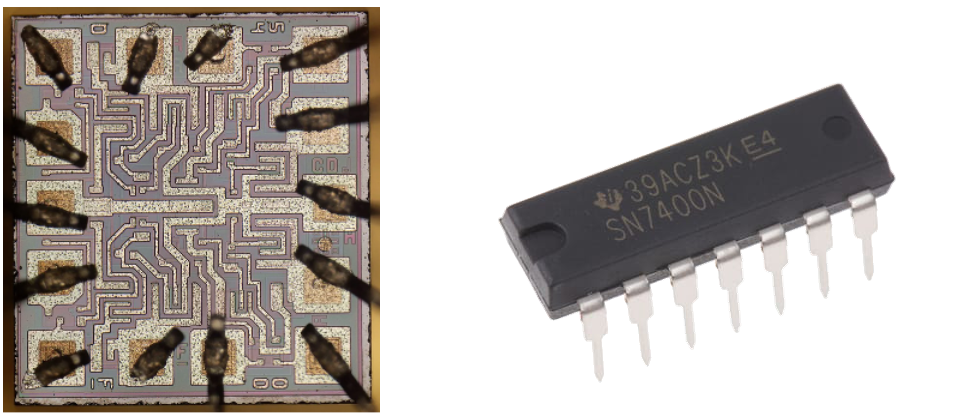
\includegraphics[width=0.40\textwidth]{lab-reports/Schematics-and-graphics/SN7400N.png}
\caption{Fotografia del DIE e del \textit{package} plastico DIP \textit{(Dual Inline Package)} dell'integrato con 2 porte NAND SN7400N}
\label{fig:integrated_nand}
\end{center}
\end{figure}

\subsection{Transistor di interfaccia PN2222A}
Gli integrati logici appena descritti, appartenendo alla famiglia TTL con stato alto a 5V, non possono essere collegati direttamente all'uscita degli amplificatori operazionali presenti nello stadio analogico del SAR, che operano tra +15V e -15V, si rende quindi necessaria l'introduzione di un transistor di interfaccia come il PN2222A, un BJT NPN \textit{general purpose} con $h_{fe}$ compreso tra 100 e 300 che tollera correnti di collettore fino a 600 mA. Questo dispositivo verrà utilizzato in configurazione ad emettitore comune in modalità interdizione / saturazione.
\cite{I}


\subsection{Integrato di \textit{sample holding} LF398}
Il convertitore SAR tratttato in questa relazione può campionare segnali variabili nel tempo sotto l'ipotesi di piccole variazioni di questi durante ciascun ciclo di campionamento e questo implica di utilizzare una frequenza di campionamento molto maggiore della frequenza delle armoniche di Fourier del segnale in ingresso. Per ottenere prestazioni migliori, raggiungendo il limite posto dal teorema di campionamento di Nyquist-Shannon, è necessario introdurre un circuito in grado di mantenere costante la tensione all'ingresso dell'ADC fino a quanto il ciclo di conversione non viene completato. Questo viene realizzato mediante l'integrato monolitico \textit{sample and hold} LF398, che prevede un ingresso compatibile con la logica TTL per controllare la finestra di campionamento, due pin per il collegamento del condensatore che permetterà il mantenimento della tensione in uscita, due pin di alimentazione duale $\pm$ 15V e naturalmente i pin di ingresso e di uscita del segnale analogico. L'integrato necessita di meno di 10 $\mu s$ per effettuare il campionamento e il datasheet riporta una stabilità del guadagno pari allo 0.002 \%.
\cite{J}

\subsection{Scheda a microcontrollore}
Nell'ultima fase dell'esperienza di laboratorio verrà realizzato un semplice sistema di registrazione dei valori acquisiti utilizzando un microcontrollore \textit{Atmel ATmega328P} basato sull'architettura Harvard RISC a 8 bit interfacciato con un lettore di schede microSD. Questo MCU viene impiegato con un oscillatore esterno al quarzo a 16 MHz per il clock, dispone di 32 KB di memoria ISP flash e nel nostro caso è installato su una scheda Arduino che ospita anche un secondo microcontrollore \textit{Atmel ATmega16u2} con funzione di interfaccia di programmazione USB. La funzione di questo dispositivo è quella di leggere lo stato delle uscite dei J-K, corrispondente alla rappresentazione binaria del segnale campionato, e di scrivere su un file salvato una scheda microSD a cui è connesso mediante una linea seriale SPI.

%%%%%%%%%%%%%%%%%%%%%%%%%%%%%%%%%%%%%%%%%%%%%%%%%%%%%%%%

\section{Caratterizzazione dei circuiti logici fondamentali}
Si verificheranno rapidamente in laboratrio alcune caratteristiche significative di alcuni circuiti logici fondamentali, alcuni verranno utilizzati successivamente per la realizzazione dell'ADC.

\subsection{Verifica della tabella di verità della porta AND}
Una porta AND è un gate logico con due o più ingressi e un'uscita che esegue l'operazione di congiunzione logica. L'output di tale componente rispetta, infatti, la seguente tabella di verità:
\begin{center}
\begin{tabular}{ |c|c|c| } 
 \hline
 \rowcolor{lightgray}
 A & B & OUT \\ \hline \hline
 0 & 0 & 0 \\ \hline
 1 & 0 & 0 \\ \hline
 0 & 0 & 0 \\ \hline
 1 & 1 & 1 \\ \hline
 
 \hline
\end{tabular}
\end{center}
In laboratorio utilizzando l'integrato \textbf{SN74LS08N} e fornendo in ingresso due onde quadre di frequenza 5 Hz oscillanti tra 0 e 5 V e sfasate di un quarto di periodo si è ottenuto il grafico in  \textit{figura \ref{fig:AND-table}} 
\begin{figure}[H]%[!ht]
\begin{center}
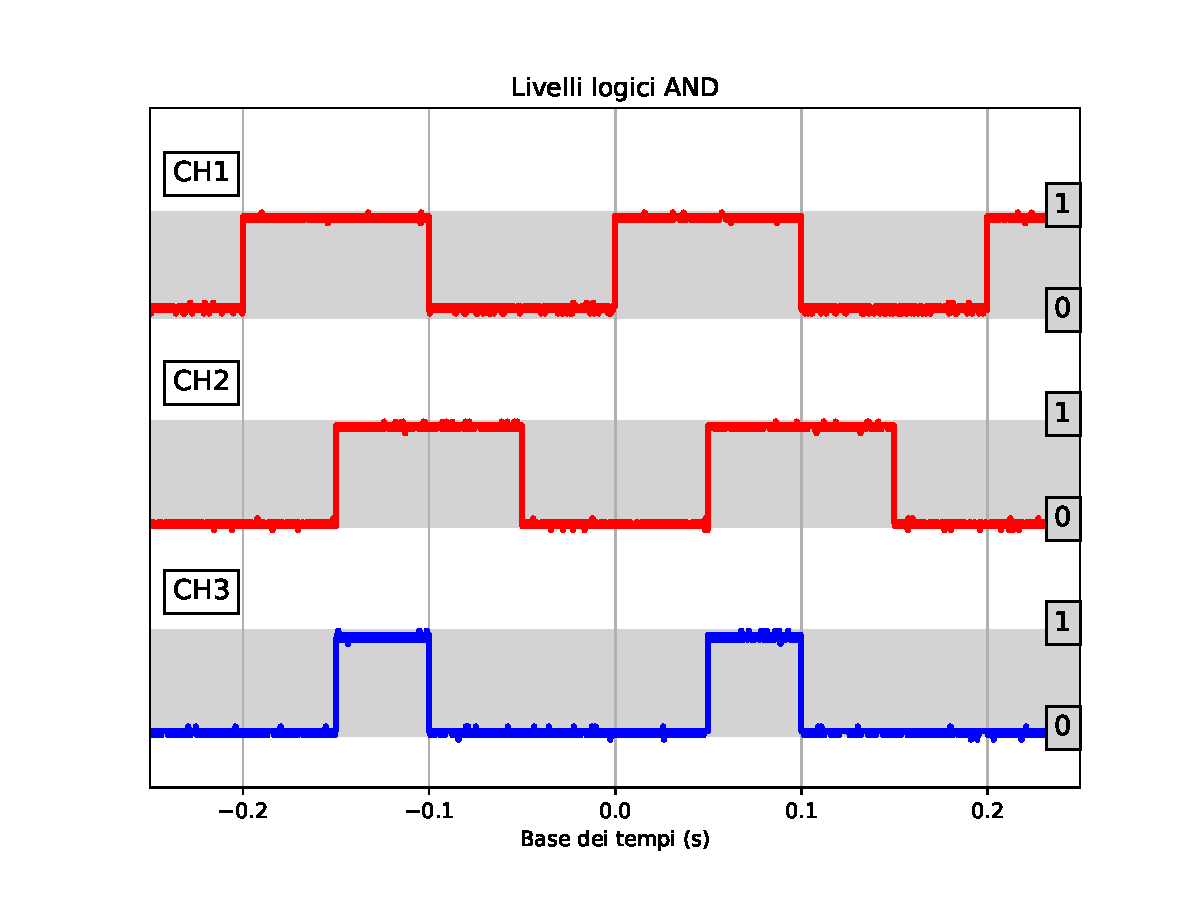
\includegraphics[width=0.50\textwidth]{analysis/output/AND-all.pdf}
\caption{Verifica della tabella di verità della porta logica AND}
\label{fig:AND-table}
\end{center}
\end{figure}

Lo sfasamento introdotto fa sì che si verifichino tutte le possibili combinazioni di stati logici agli ingressi A e B, permettendo la verifica dell'intera tabella di verità. Si osserva, in particolare, che l'uscita è allo stato alto solo quando lo sono sia A che B.


\subsection{Studio della caratteristica di trasferimento della porta NOT}

\begin{figure}[H]%[!ht]
\begin{center}
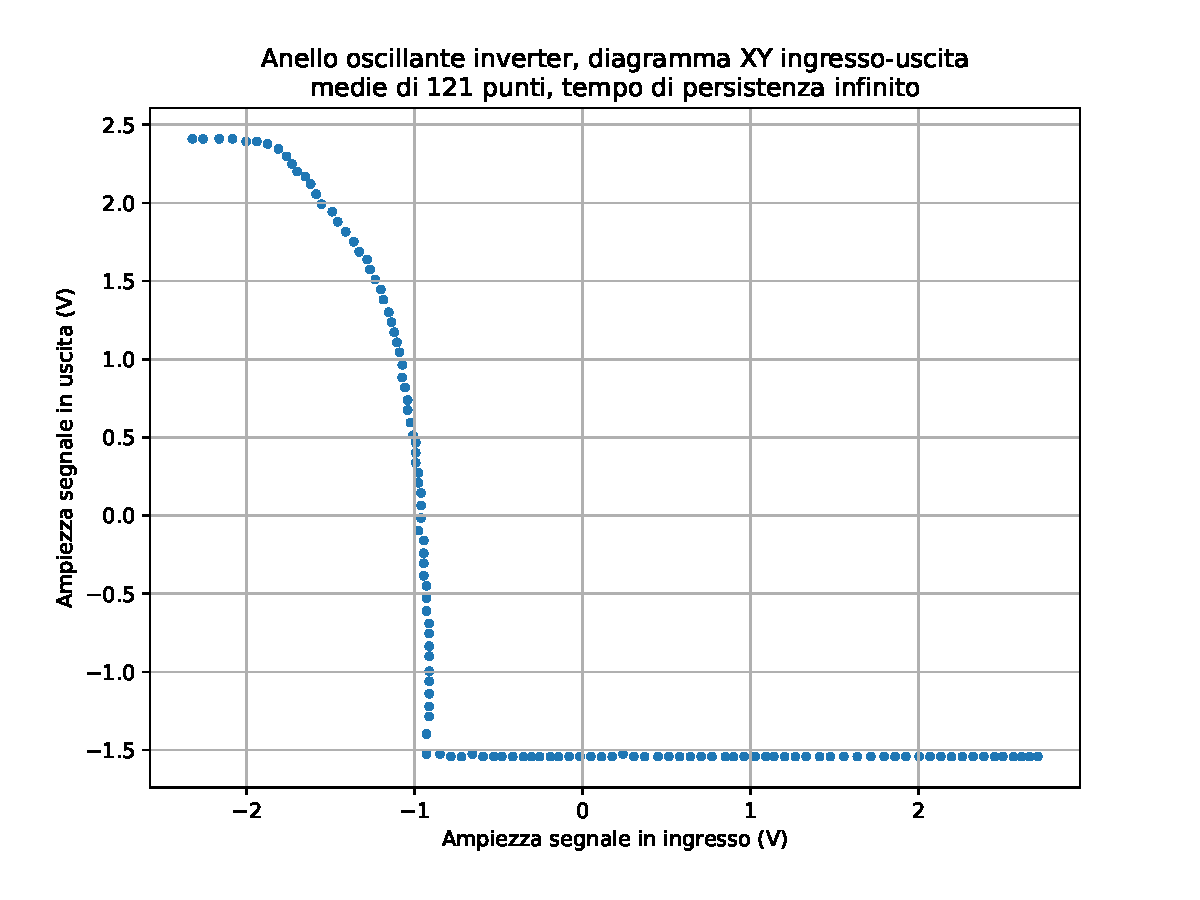
\includegraphics[width=0.45\textwidth]{analysis/output/inverter_ring_xy.pdf}
\caption{Caratteristica di trasferimento della porta NOT}
\label{fig:transf_not}
\end{center}
\end{figure}

Passiamo ora allo studio della caratteristica di trasferimento della porta NOT, rappresentata in textit{figura \ref{fig:transf_not}}
, dove sull'asse orizzontale troviamo la tensione in ingresso e sull'asse verticale la tensione in uscita. La forma del fronte di discesa che distingue il livello di uscita alto dal livello di uscita basso è di fondamentale importanza per il buon funzionamento della porta logica, perché consente una progressiva rigenerazione di un segnale logico attenuato o affetto da rumore, man mano che esso attraversa più porte logiche, anziché un suo ulteriore degrado. Supponiamo infatti di avere un segnale logico basso (0 V) affetto da un rumore ampio 1 V che attraversa un buffer formato con due porte NOT in serie: dal grafico si osserva che la prima mapperà 1 V a 3.3 V circa, mentre la seconda mapperà 3.3 V precisamente a 0 V. Si è ottenuto così un effetto di reiezione del rumore.




\subsection{Studio della caratteristica di trasferimento della porta NAND}
Ripetiamo ora la medesima analisi per la porta NAND fissando un ingresso al livello alto 5 V e collegando, come già fatto in precedenza, l'altro ingresso al generatore di segnali impostato per produrre una rampa da 0 V a 5 V a f = 500 Hz. La figura è prodotta dall'oscilloscopio in modalità di visualizzazione XY con il canale orizzontale collegato all'uscita del generatore e il canale verticale all'uscita della porta NAND. Osserviamo una zona particolarmente rumorosa nell'intorno della tensione a cui la porta NAND effettua la commutazione e osserviamo che anche con l'uscita scollegata da qualsiasi carico la porta NAND non raggiunge i 5 V in uscita previsti dallo standard TTL, ciò nonostante la posizione della soglia di commutazione a circa 1 V garantisce la corretta interpretazione di segnali alti con ampiezza 4 V.

\begin{figure}[H]%[!ht]
\begin{center}
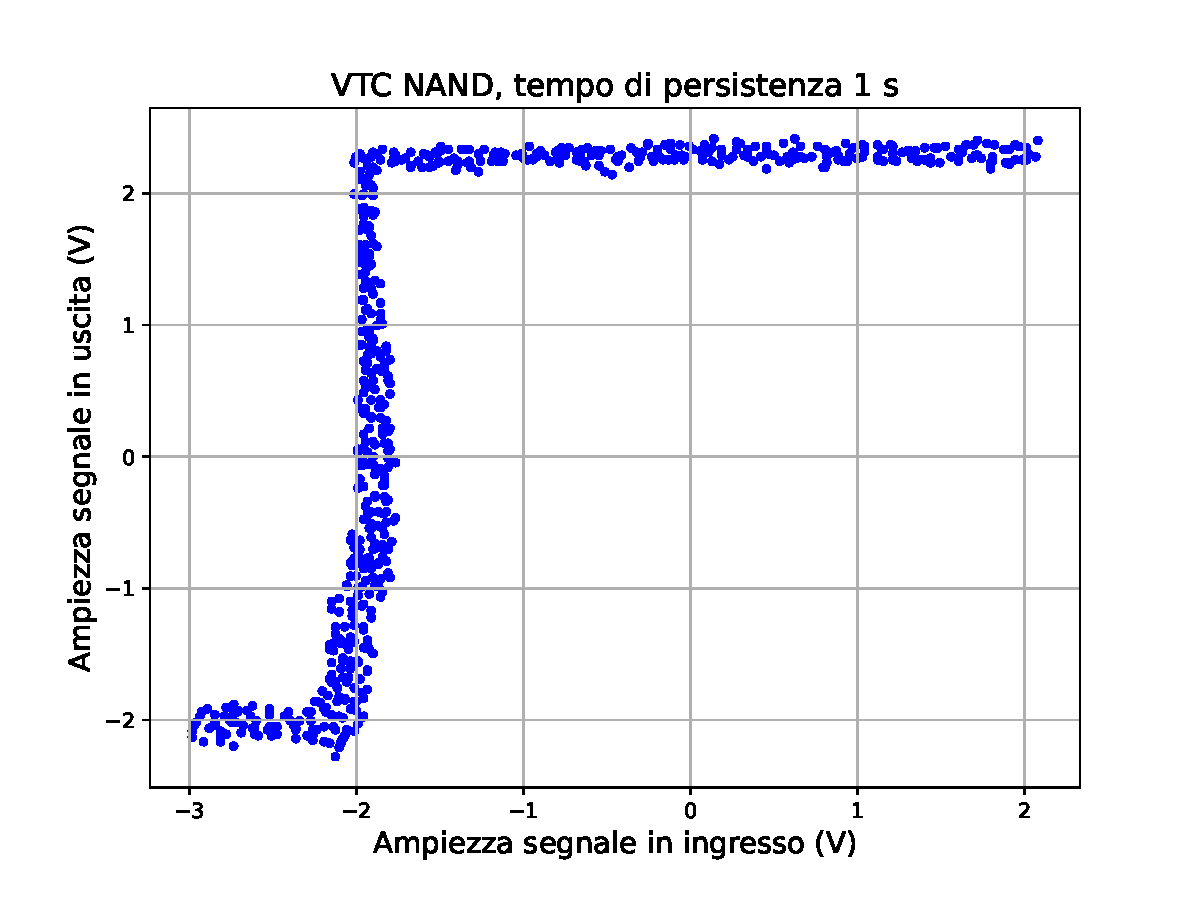
\includegraphics[width=0.45\textwidth]{analysis/output/NAND-XY.pdf}
\caption{Forma d'onda generata dal gate NAND}
\label{fig:graph_ring_oscillator}
\end{center}
\end{figure}


\subsection{Flip-flop di tipo set - reset}
\begin{figure}[H]%[!ht]
\begin{center}
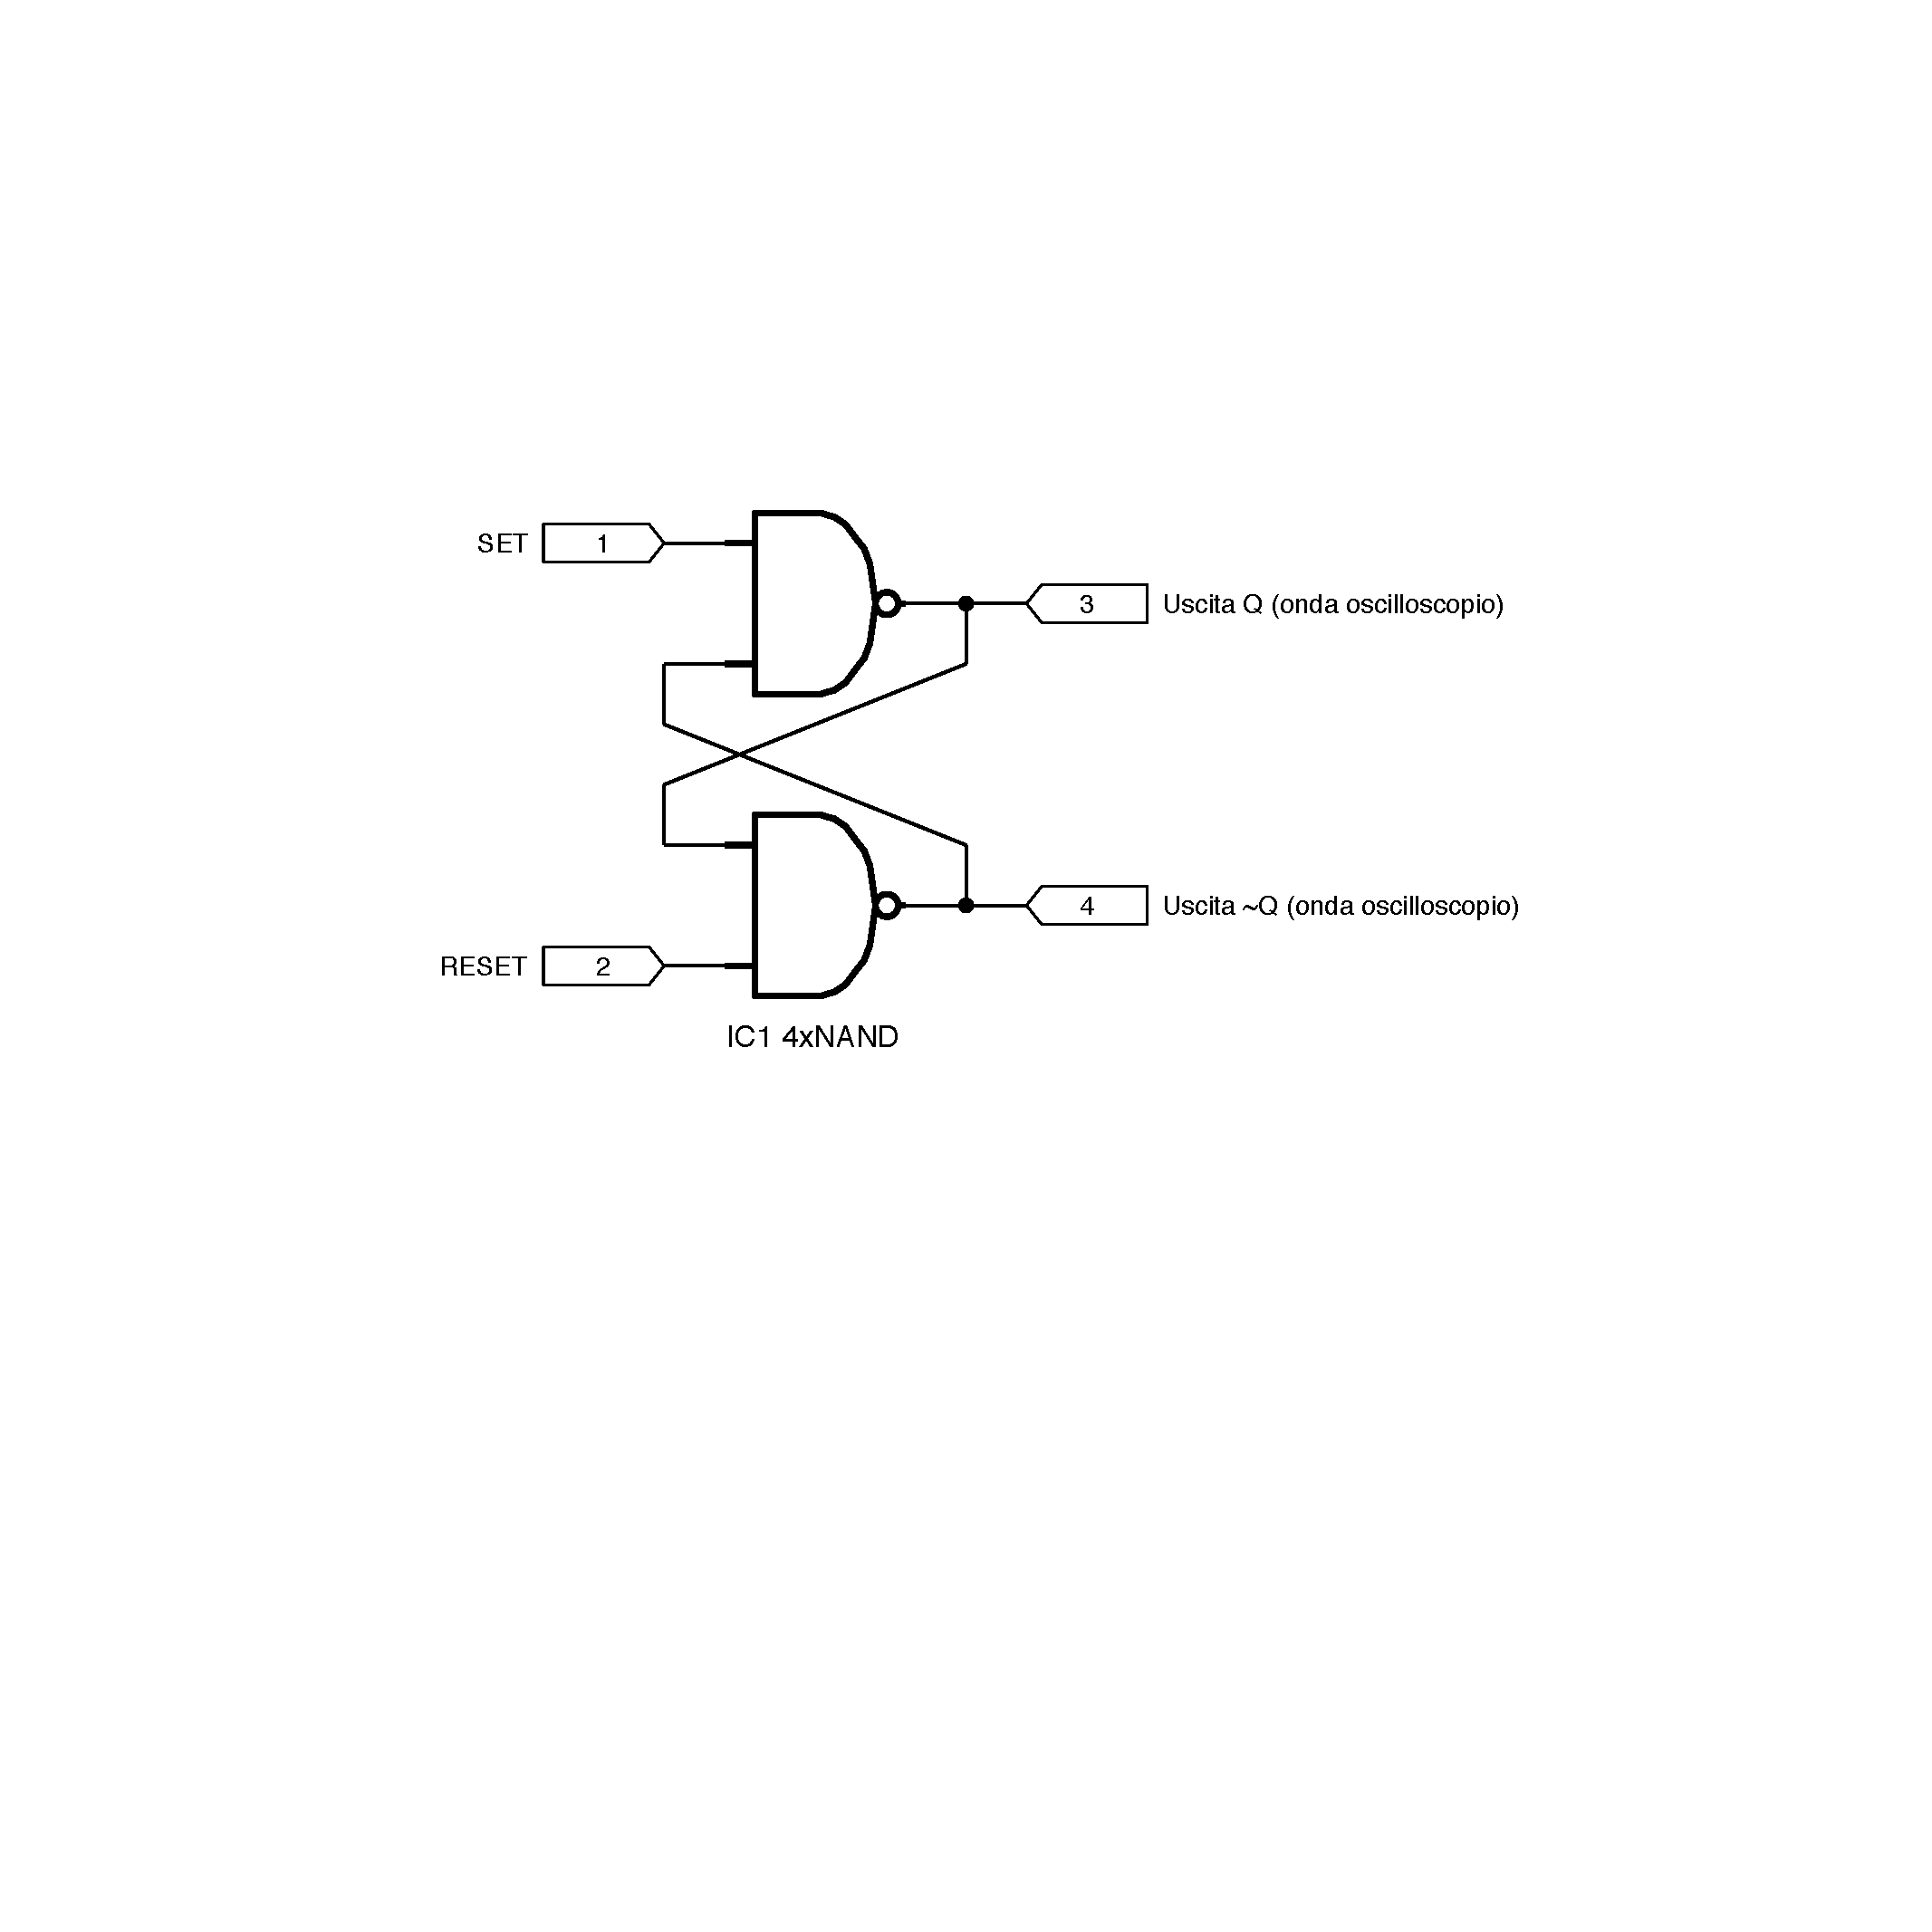
\includegraphics[width=0.30\textwidth]{sch-simulations/digital/output/flip-flop-RS.pdf}
\caption{Logica interna del flip-flop set-reset}
\label{fig:circuit_flip_flop}
\end{center}
\end{figure}
Il \textit{Flip-Flop SR }, noto  anche come \textit{SR latch}, è uno dei circuiti digitali sequenziali fondamentali, si tratta di un dispositivo di memoria bistabile a singolo bit. E' dotato di due ingressi: \textit{SET} e \textit{RESET}. Quando entrambi si trovano ad 1 il flip flop si trova in stato di memoria, cioè lo stato delle uscite Q e Q negato viene mantenuto costante, mentre quando uno tra gli ingressi SET e RESET viene portato a 0 l'uscita Q passa rispettivamente allo stato 1 o allo stato 0.
Il comportamento di un SR NAND Flip-Flop è quindi regolato dalla seguente tavola di verità:
\begin{center}
\begin{tabular}{ |c|c|c|c|c| } 
 \hline
 \rowcolor{lightgray}
S & R & Q & $\overline{Q}$ &\\ \hline \hline
 0 & 0 & 1 & 1 & Impredicibile\\  \hline
 0 & 1 & 1 & 0 & Stato stabile\\ \hline
 1 & 0 & 0 & 1 & Stato stabile\\ \hline
 1 & 1 & 0 & 1 & Memoria\\ \hline
 1 & 1 & 1 & 0 & Memoria\\ \hline
 
 \hline
\end{tabular}
\end{center}

In laboratorio è stato implementato un flip-flop RS utilizzando due porte logiche NAND dell'integrato \textit{SN74LS00N} e si è potuta verificare la tabella di verità osservando i segnali misurati con l'oscilloscopio mostrati nelle figure seguenti.

\begin{figure}[H]%[!ht]
\begin{center}
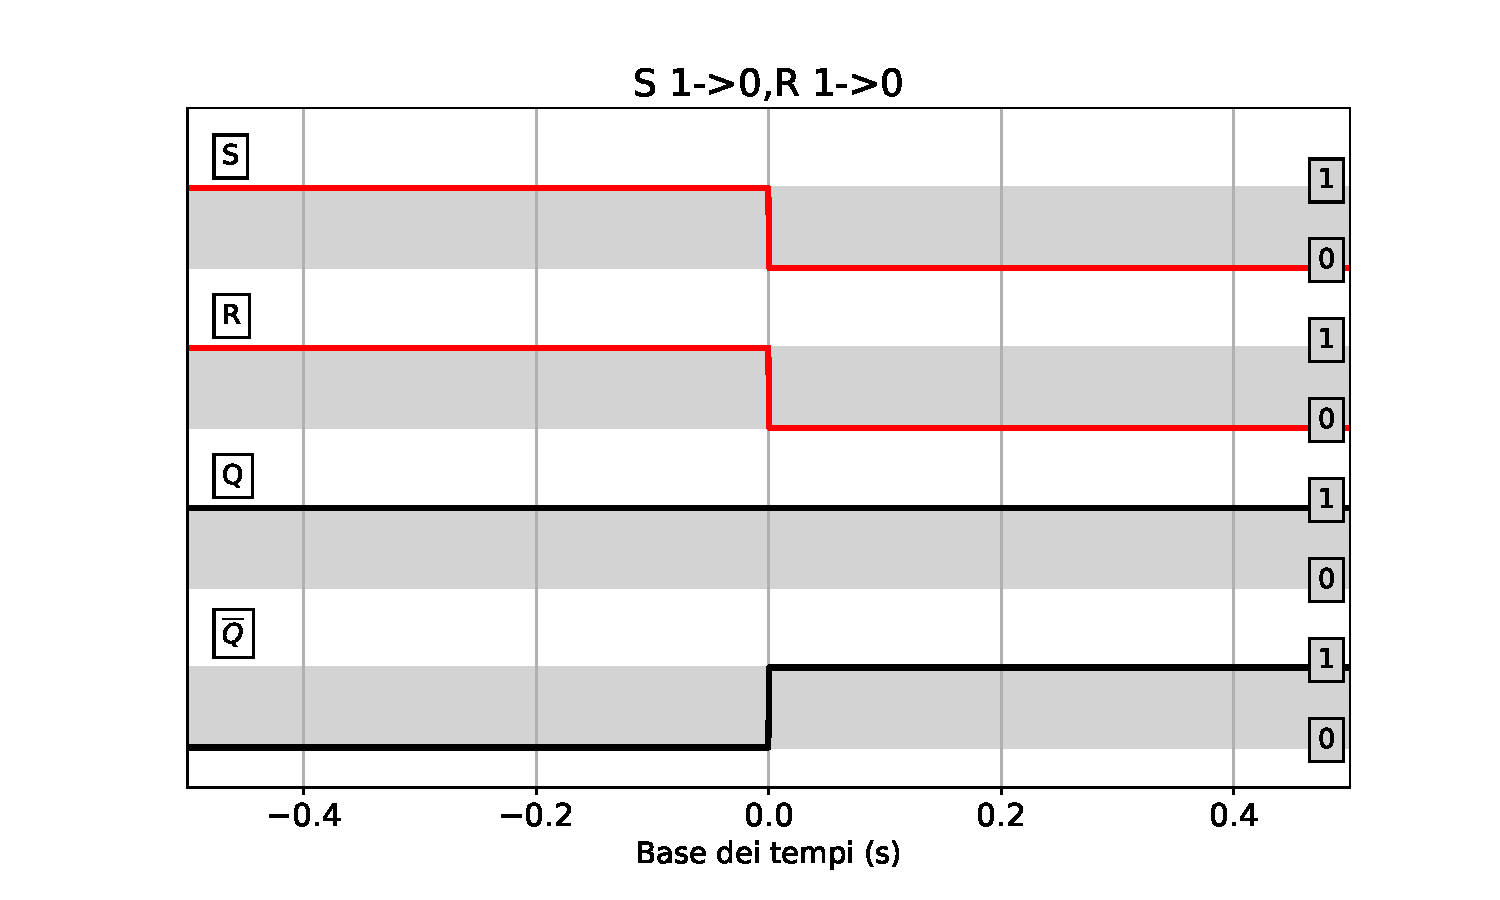
\includegraphics[ width=0.48\textwidth]{analysis/output/set-reset-to-0_0.pdf}
\label{fig:SR}
\end{center}
\end{figure}

\begin{figure}[H]%[!ht]
\begin{center}
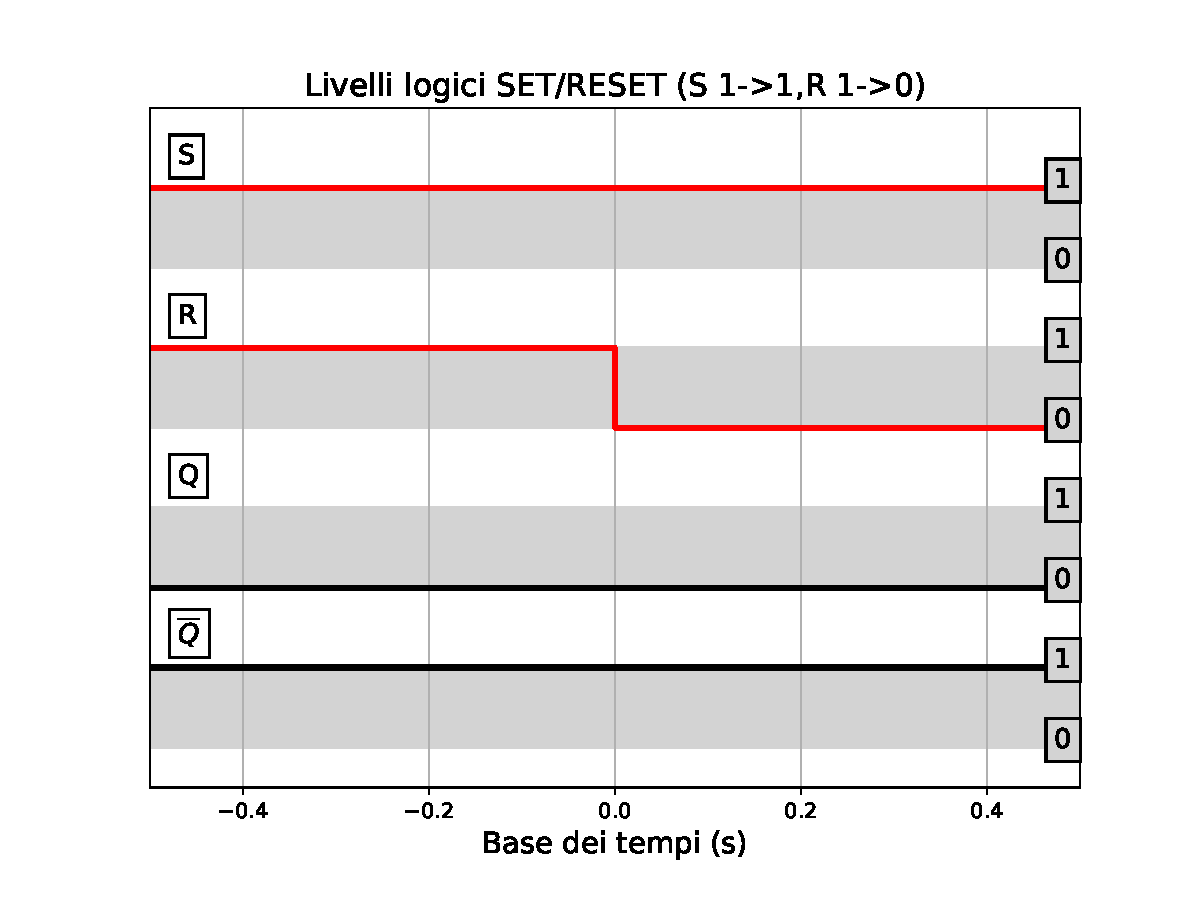
\includegraphics[ width=0.48\textwidth]{analysis/output/set-reset-to-1_0.pdf}
\label{fig:SR}
\end{center}
\end{figure}

\begin{figure}[H]%[!ht]
\begin{center}
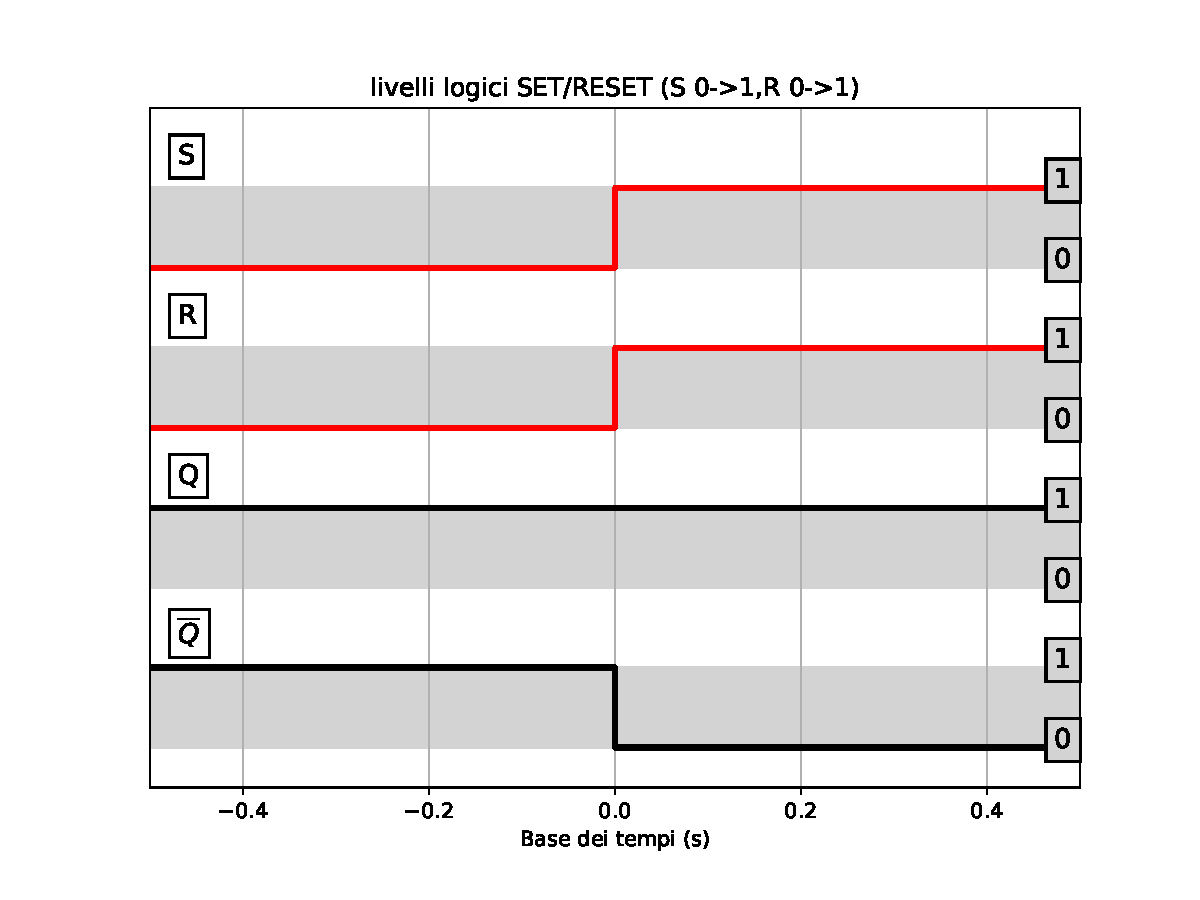
\includegraphics[ width=0.48\textwidth]{analysis/output/set-reset-to-1_1.pdf}
\label{fig:SR}
\end{center}
\end{figure}

\begin{figure}[H]%[!ht]
\begin{center}
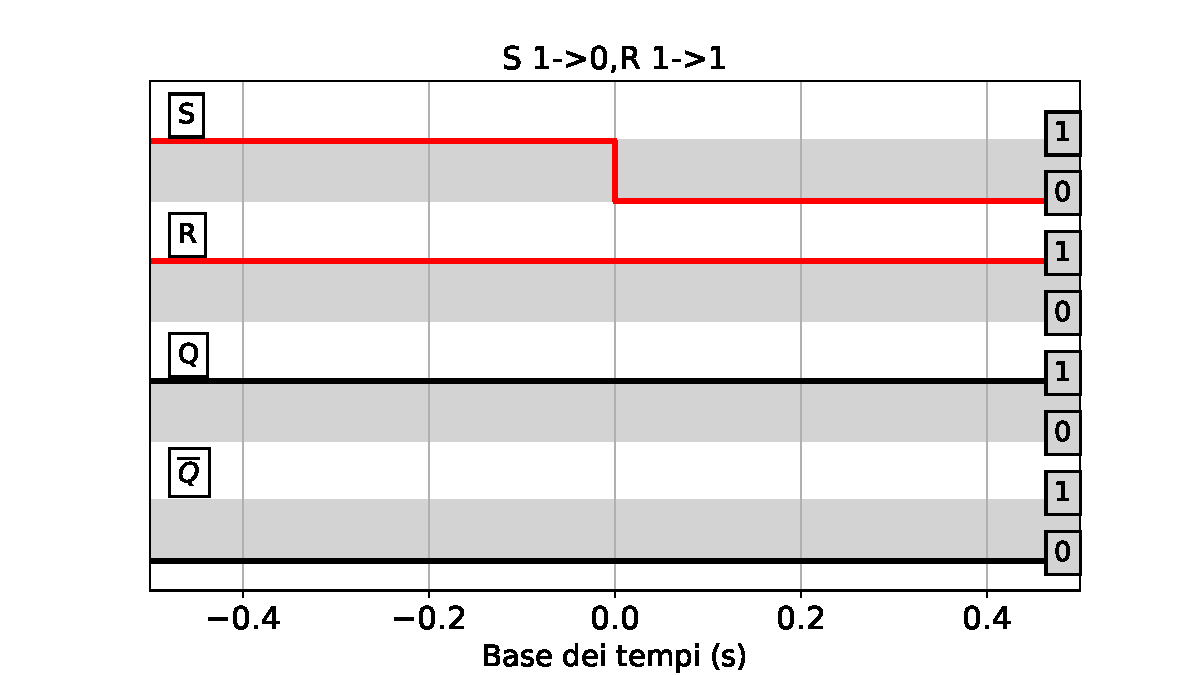
\includegraphics[ width=0.48\textwidth]{analysis/output/set-reset-to-0_1.pdf}
\caption{Verifica della tabella di verità di un flip-flop di tipo set-reset realizzato con porte NAND}
\label{fig:SR}
\end{center}
\end{figure}

%\begin{figure}[H]%[!ht]
%\begin{center}
%\includegraphics[trim = {0 0 580 0}, clip, %width=0.37\textwidth]{analysis/output/set-reset-table.pdf}
%porte NAND}
%\label{fig:SR-1}
%\end{center}
%\end{figure}


%\begin{figure}[H]%[!ht]
%\begin{center}
%\includegraphics[trim = {580 0 0 0}, clip, width=0.37\textwidth]{analysis/output/set-reset-table.pdf}
%\caption{Verifica della tabella di verità di un flip-flop di tipo set-reset realizzato con porte NAND}
%\label{fig:SR-2}
%\end{center}
%\end{figure}

Notiamo dalla \textit{figura \ref{fig:SR}} che il dispositivo si comporta nel modo atteso, verificando in ogni situazione i livelli logici predetti.
Questo dispositivo presenta però due limitazioni:
\begin{itemize}
    \item Lo stato con ingressi entrambi a 0 è impredicibile perché dipende dall'istante di tempo in cui il primo passa al valore basso e questo dipende tipicamente dal rumore; questo stato non viene praticamente mai utilizzato.
    \item L'operazione di latching avviene in modo asincrono, cioè appena uno degli ingressi si porta allo stato basso, non è previsto un ingresso di \textit{clock} che controlla l'istante di commutazione.
\end{itemize}
\subsection{Verifica della tabella di verità del flip-flop di tipo J-K}

Il \textit{JK Flip-Flop} è uno dei  flip-flop più diffusi nei circuiti digitali. Presenta due input \textit{J} e \textit{K} con funzioni analoghe al SET e RESET del latch visto in precedenza; tale dispositivo è in grado di superare entrambe le limitazioni prima elencate per quest'ultimo. Si tratta, infatti, di un flip-flop SR dotato di porte NAND a tre ingressi (realizzate con transistor ad emettitore triplo), che permettono sia l'introduzione di un segnale di \textit{clock} l'aggiunta di due nuovi circuiti di feedback dalle uscite che eliminano lo stato impredicibile sostituendolo con l'operazione di \textit{toggle}. Vi sono quindi quattro combinazioni logiche possibili per gli ingressi, riportate nella tabella di verità sottostante.
\newline
\begin{center}
\begin{tabular}{ |c|c|c|c|c| } 
 \hline
 \rowcolor{lightgray}
 J & K & Q & $\overline{Q}$ & $ Q_{n + 1} $ \\ \hline \hline
 0 & 0 &  &  & $Q_n$ \\ \hline
 1 & 0 & 0 & 1 & 1 \\ \hline
 1 & 0 & 1 & 0 & 1\\ \hline
 0 & 1 & 0 & 1 & 0 \\ \hline
 0 & 1 & 1 & 0 & 0 \\ \hline
 1 & 1 &  & & $\overline{Q_n}$ \\ \hline
\end{tabular}
\end{center}

\begin{figure}[H]%[t]
\centering
\begin{center}
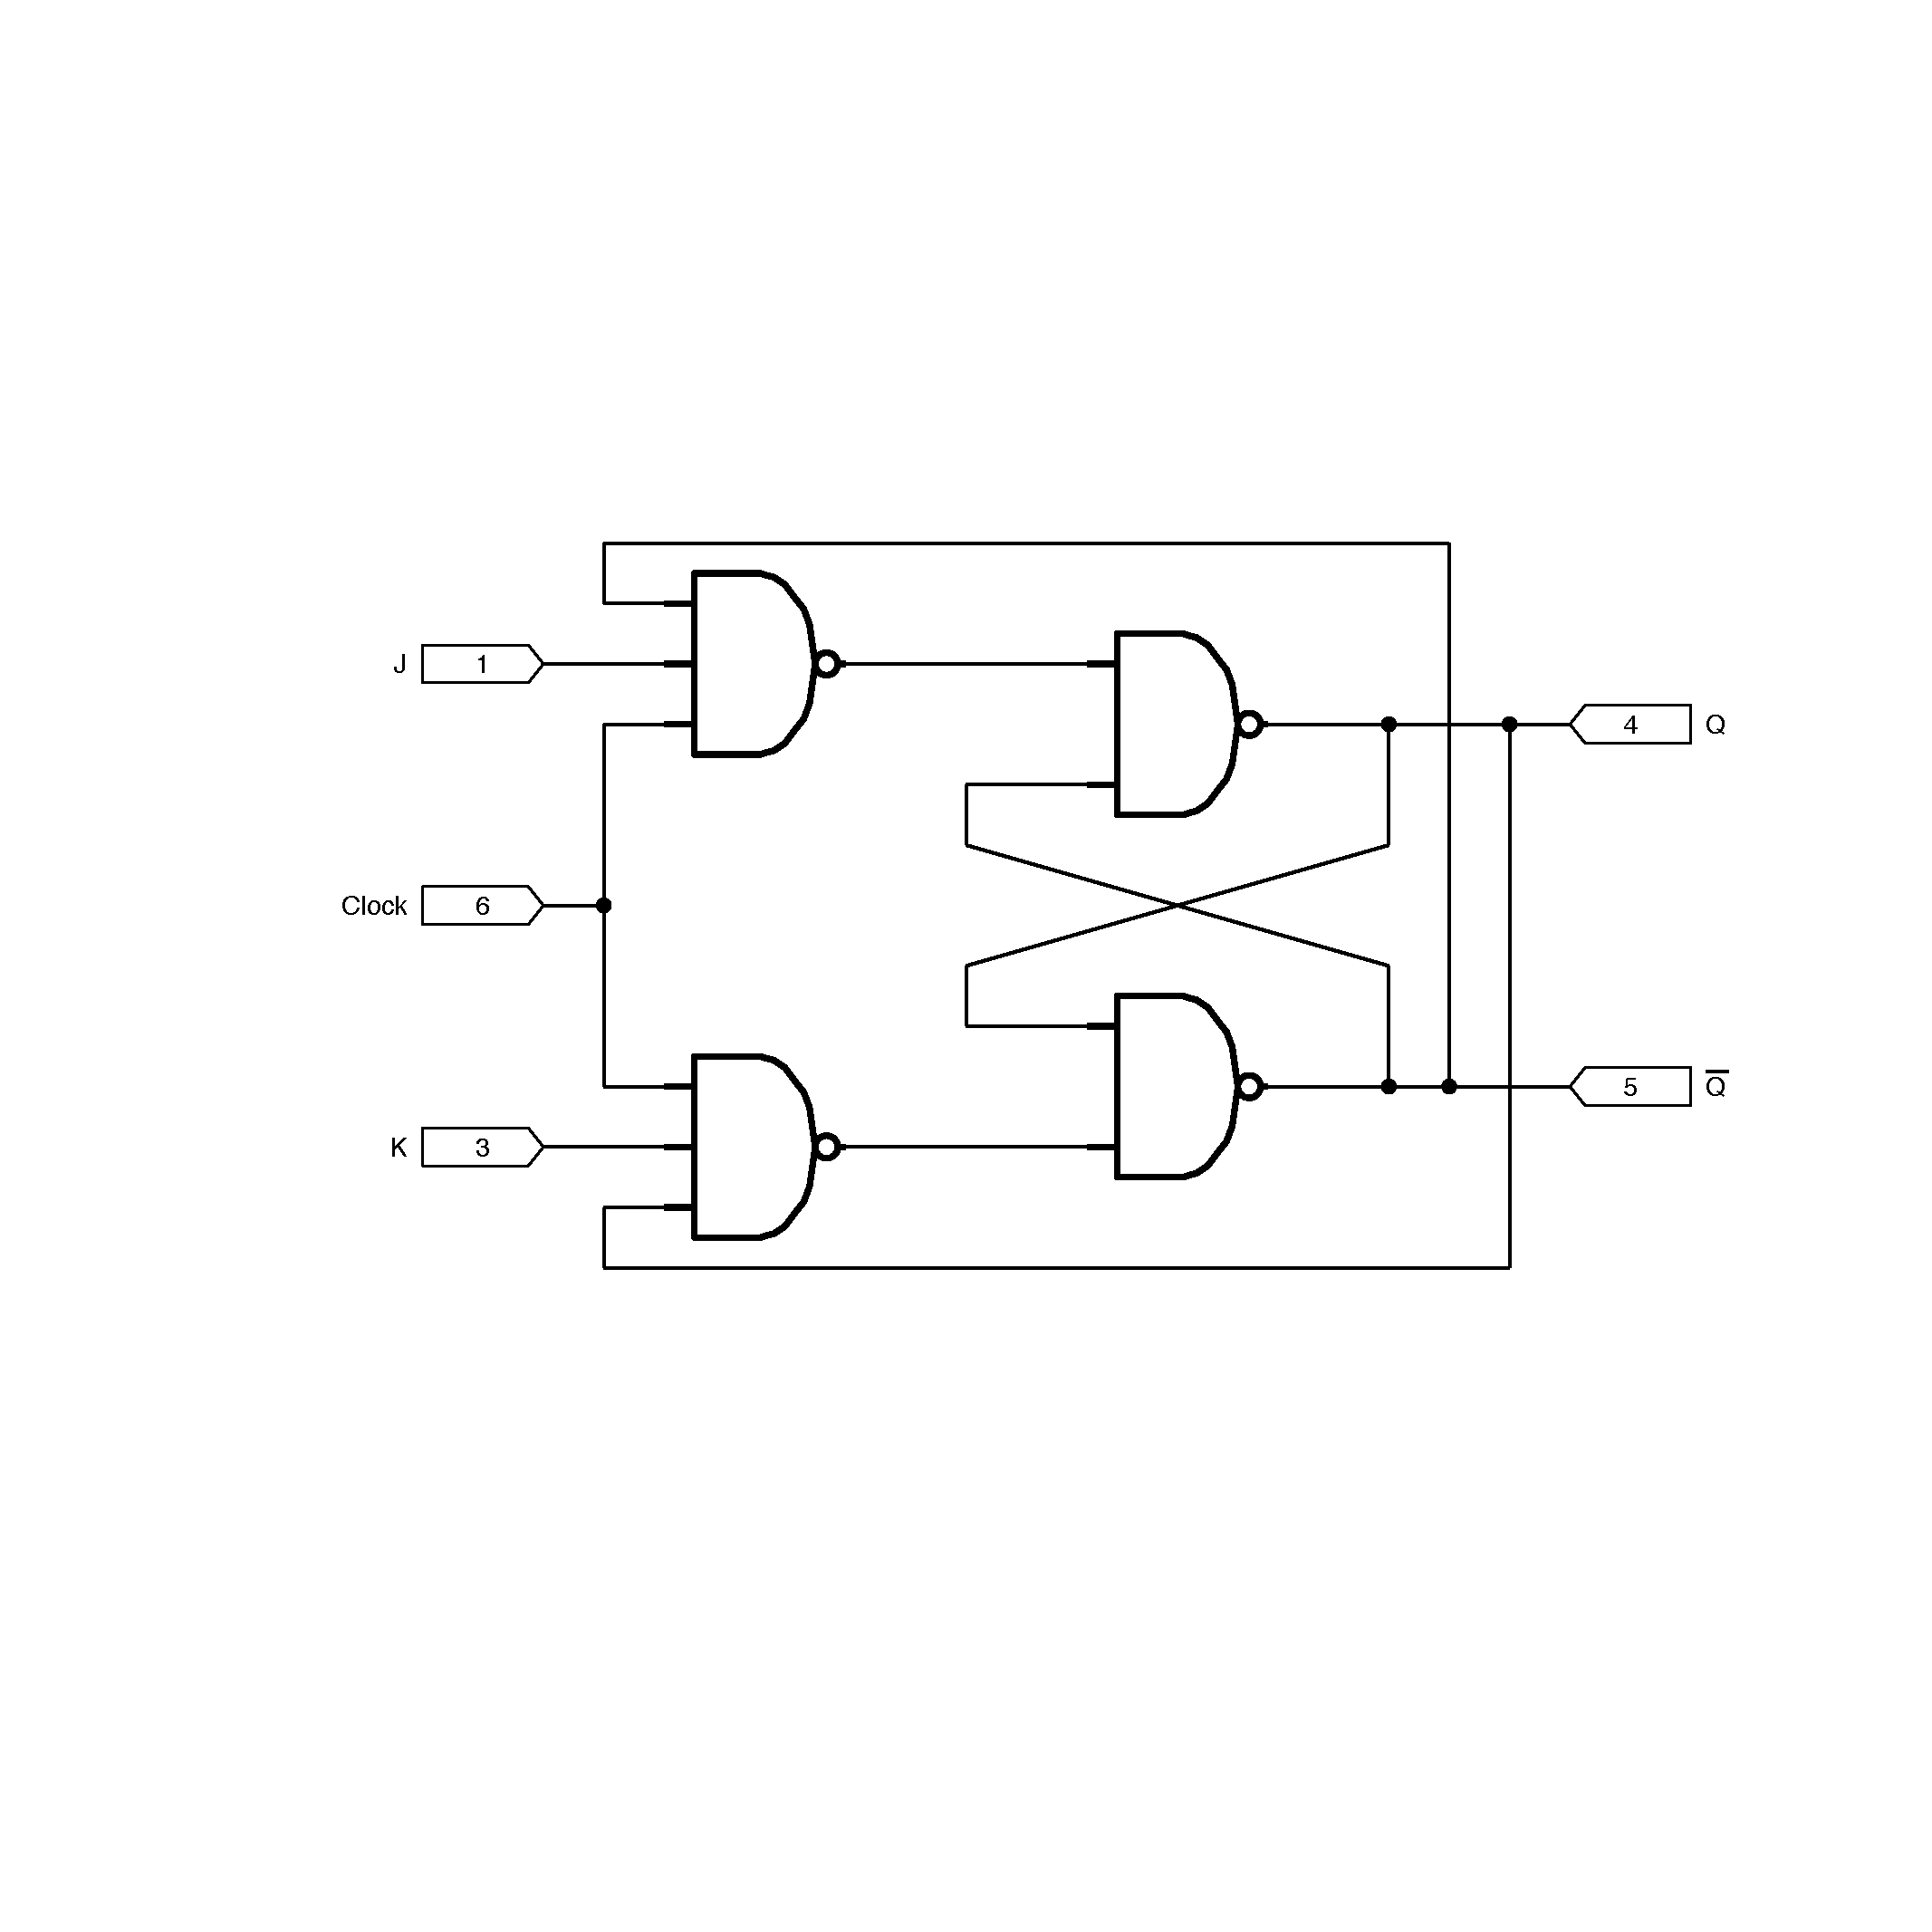
\includegraphics[width=0.40\textwidth]{sch-simulations/digital/output/flip-flop-JK.pdf}
\end{center}
\caption{Logica interna del flip-flop JK}
\label{fig:circuit_JK}
\end{figure}

\begin{figure*}[t]%[t]
\centering
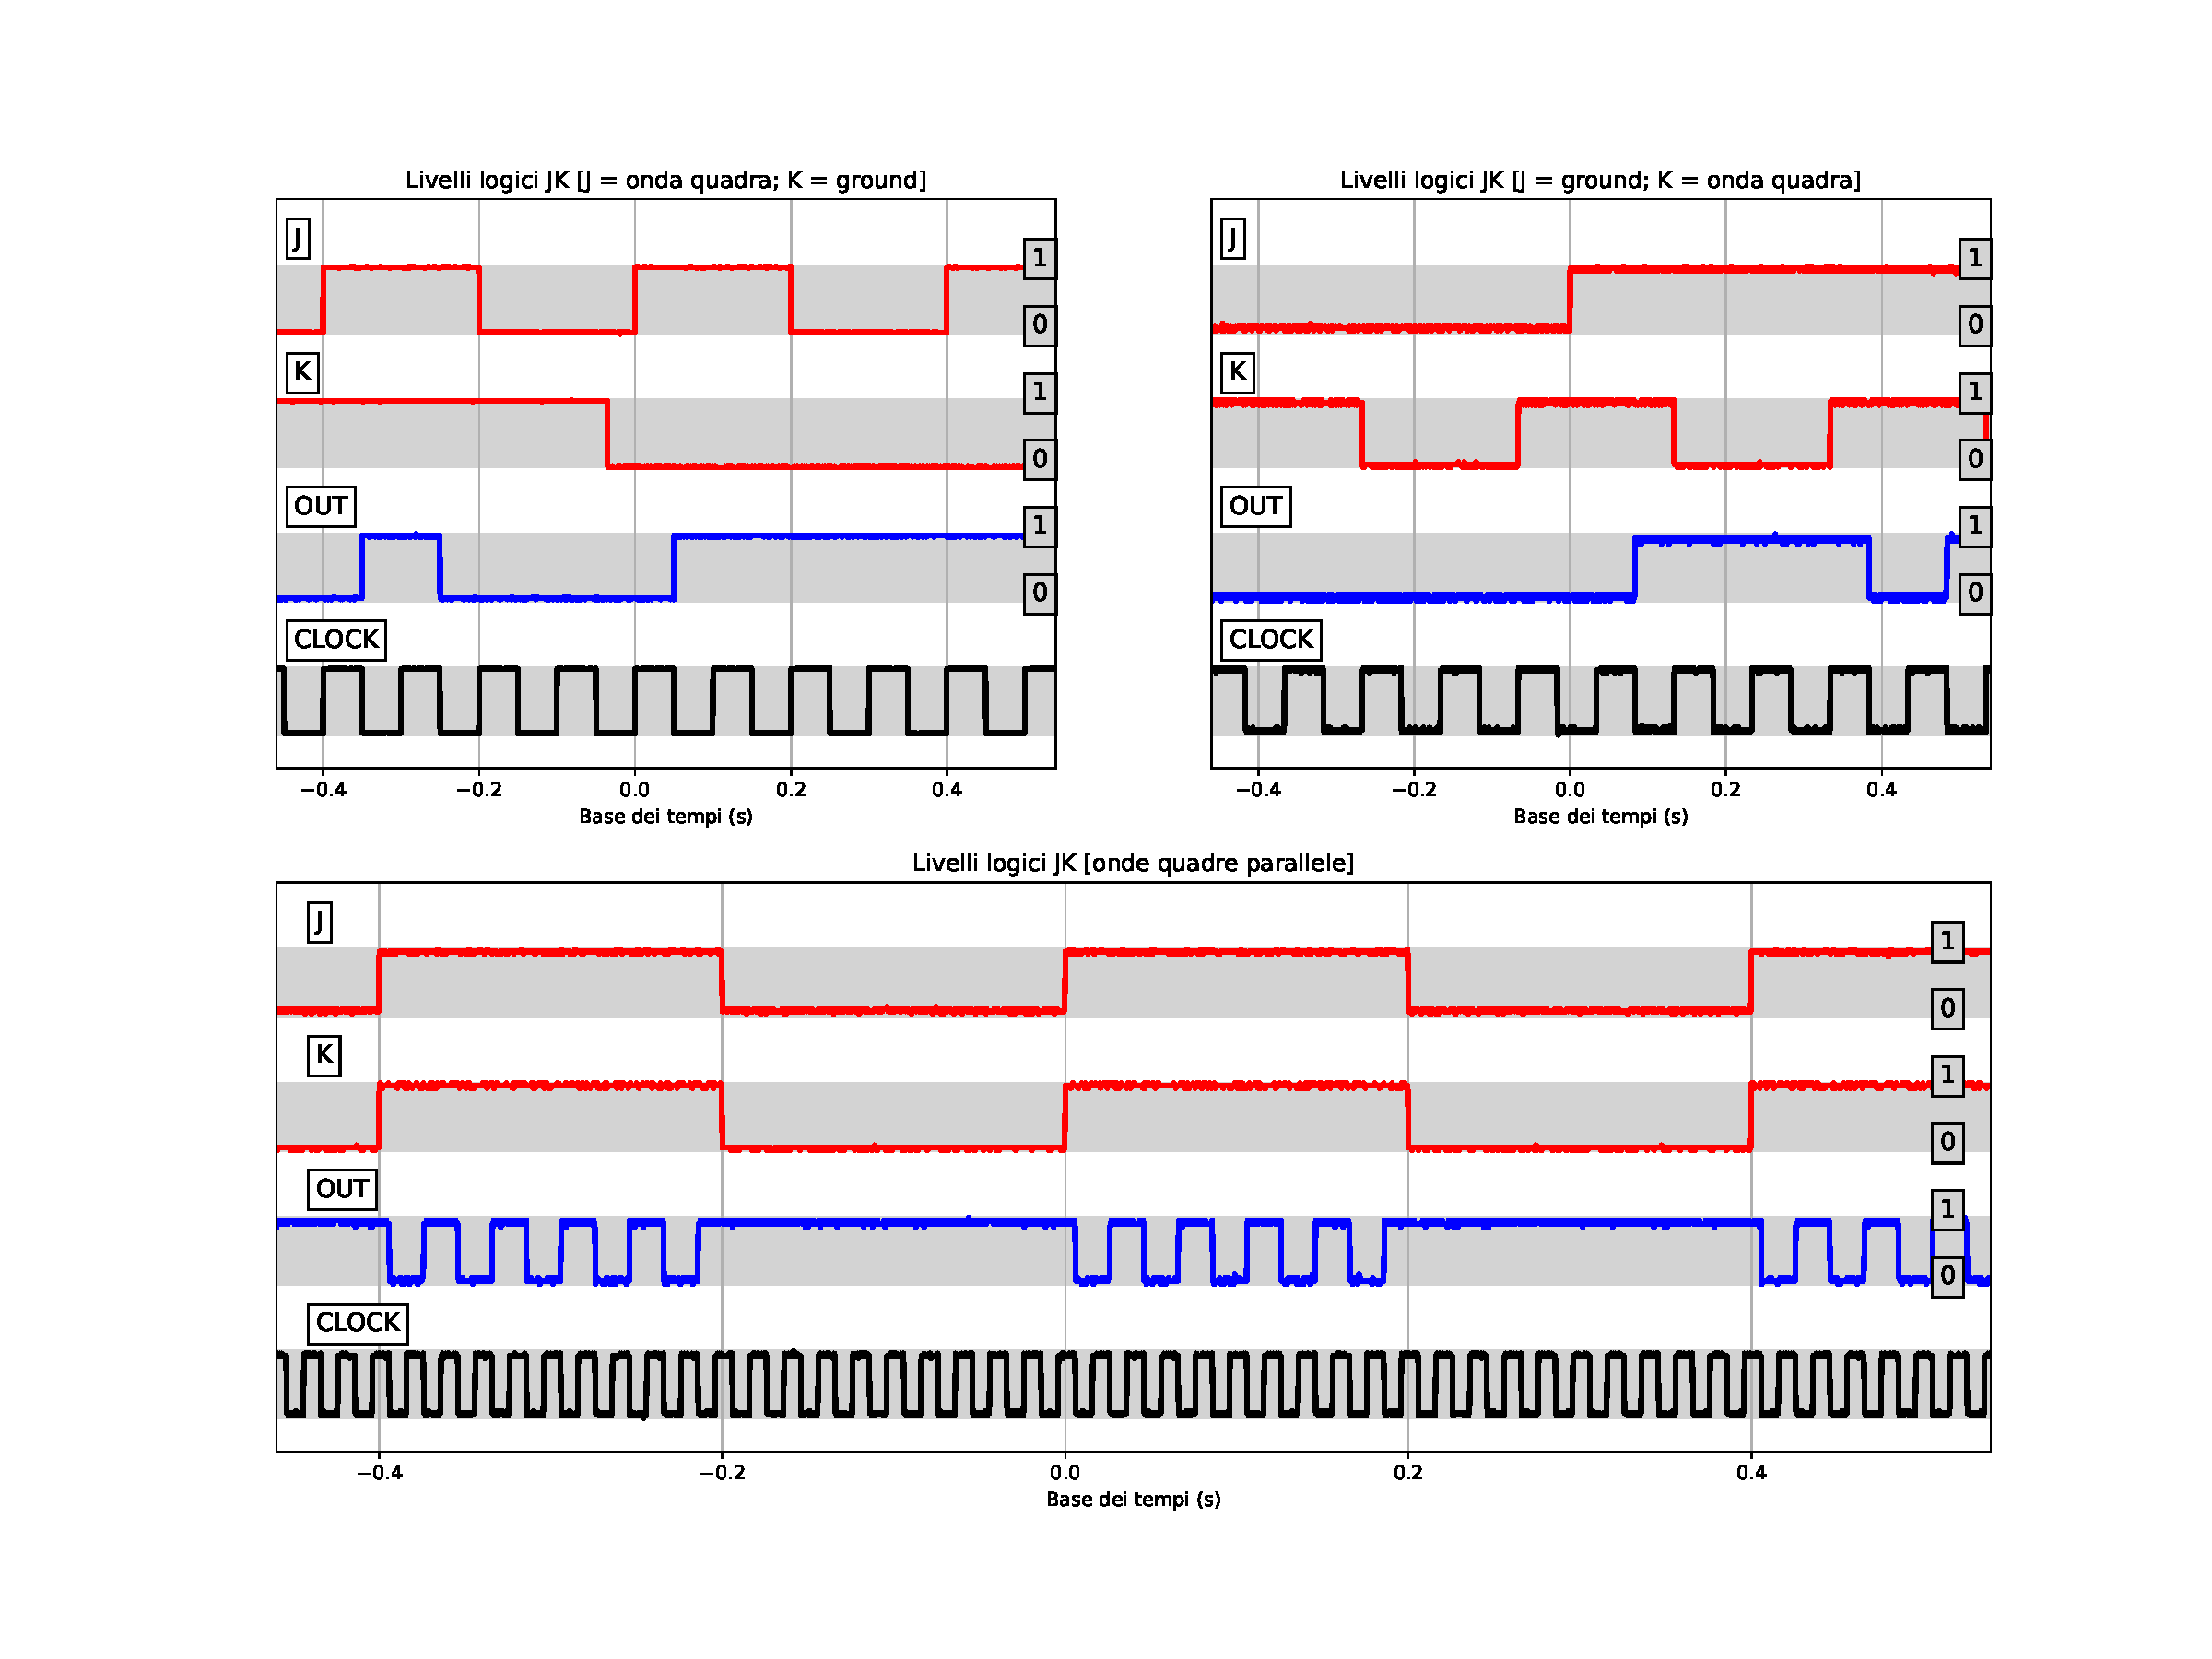
\includegraphics[width=0.95\textwidth]{analysis/output/JK-truth.pdf}
\caption{Verifica della tabella di verità di un flip-flop di tipo J-K}
\label{fig:jk-truth}
\end{figure*}
Discutiamo ora brevemente la verifica effettuata in laboratorio con l'integrato 74LS76AN.
Anche in questo caso il comportamento dell'integrato è quello atteso. Aspetti importanti da osservare sono in primo luogo il fatto che il cambio dei valori logici degli ingressi viene registrato nell'output solo dopo un fronte del \textit{clock} (nel nostro caso si tratta di un \textit{negative-edge flip-flop}) come ben evidente nei primi due grafici della \textit{figura \ref{fig:jk-truth}}. Per realizzare questa misura è stato collegato in modo alterno uno dei due ingressi ad un'uscita del generatore di segnali che produceva un'onda quadra, mentre l'altro ingresso era collegato ad un pulsante e controllava anche il trigger dell'oscilloscopio. 
Nel quadrante inferiore della figura osserviamo, invece, lo stato di \textit{toggle}, che si presente nel caso di J = K = 1, che noi abbiamo ottenuto collegando in parallelo i due ingressi ad un'uscita del generatore di segnali.
%%%%%%%%%%%%%%%%%%%%%%%%%%%%%%%%%%%%%%%%%%%%%%%%%%%%%%%%

\section{Verifica del funzionamento del ring oscillator realizzato con inverter}
Come anticipato nel paragrafo di descrizione degli integrati, il dispositivo SN74LS04 che implementa 6 porte NOT presenta un tempo di commutazione non trascurabile al variare del livello logico del segnale in ingresso alle alte frequenze e questo, se realizziamo una catena di porte OR, darà origine ad un ritardo di propagazione del segnale in ogni porta. 
Questo effetto porta a conseguenze interessanti se si realizza un anello chiuso con un numero dispari di inverters, nel nostro caso 7 suddivisi su due integrati. Si osserva infatti, collegando una sonda dell'oscilloscopio ad un punto arbitrario, che alimentando gli inverter le uscite cominciano ad oscillare liberamente con una forma d'onda che ricorda un'onda triangolare distorta con un periodo proporzionale al ritardo introdotto da ogni porta e al numero delle porte. Si sottolinea che il circuito risultante è un vero e proprio oscillatore, in quanto è in grado di produrre un'uscita periodica a partire da ingressi costanti nel tempo e non necessita di alcun innesco esterno se non quello dato dal rumore.

\begin{figure}[H]%[!ht]
\begin{center}
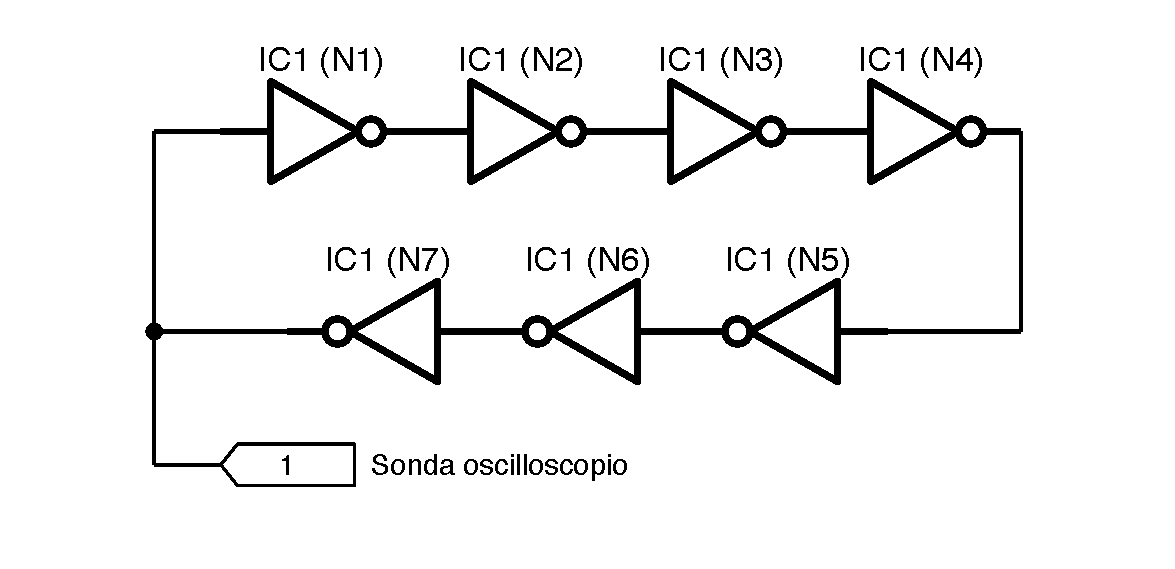
\includegraphics[width=0.40\textwidth]{sch-simulations/digital/output/ring-osc-logic.pdf}
\caption{Circuito equivalente dell'oscillatore ad anello}
\label{fig:circuit_ring_oscillator}
\end{center}
\end{figure}

Tra il ritardo di propagazione (t), il numero delle porte (n) e la frequenza della tensione oscillante generata (f) vale la presente relazione: 
\begin{math}
f = \frac{1}{2tn}
\end{math}
In laboratorio è stata acquisita la forma d'onda seguente, la cui frequenza risulta essere f = (12.66 $\pm$ 0.01) MHz, corrispondente ad un ritardo di propagazione medio tra gli inverter t = (5.6428 $\pm$ 0.0007) ns.


\begin{figure}[H]%[!ht]
\begin{center}
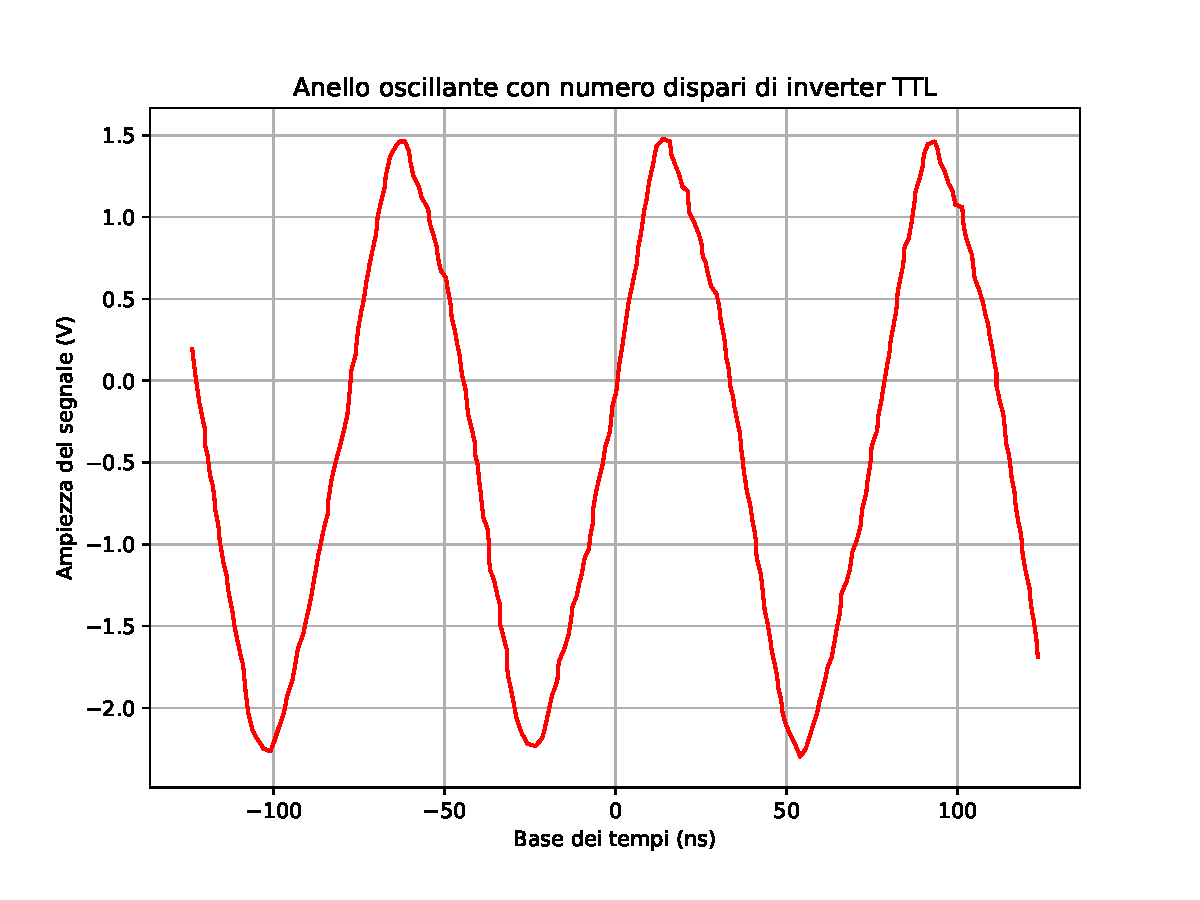
\includegraphics[width=0.50\textwidth]{analysis/output/oscillating-ring.pdf}
\caption{Forma d'onda generata dall'anello di inverter}
\label{fig:graph_ring_oscillator}
\end{center}
\end{figure}


Oscillatori di questo tipo sono utili per numerose applicazioni che spaziano dai VCO (voltage controller oscillators) dei phased-locked-loops (PLL) impiegati per generare il clock di tutte le moderne CPU fino alla generazione di numeri casuali sfruttando il jitter.

%%%%%%%%%%%%%%%%%%%%%%%%%%%%%%%%%%%%%%%%%%%%%%%%%%%%%%%%

\section{Realizzazione di un ADC SAR a 4 bit}

\subsection{Descrizione generale e specifiche tecniche desiderate}
Dopo aver preso in esame alcuni circuiti logici fondamentali, verrà ora affrontata la progettazione, calibrazione e verifica di un ADC ad approssimazioni successive (SAR) con risoluzione di 4 bit, rappresentato nello schema in figura \ref{fig:circuit_sarCompleteSchematic}. Questa tipologia di convertitori analogico - digitali è molto diffusa, sia in circuiti integrati stand alone (per esempio \textit{Analog Devices AD4695} sia all'interno di microcontrollori (per esempio la serie \textit{STM32} della \textit{ST Microelectronics}) e consente di raggiungere un buon compromesso tra frequenza di campionamento e risoluzione.

Il convertitore SAR che verrà realizzato utilizza un registro di scorrimento a 8 bit, pertanto la frequenza di campionamento sarà pari a un ottavo della frequenza di clock che durante la caratterizzazione è stata posta al massimo a 10 KHz. In questo regime di funzionamento il convertitore si è sempre mostrato affidabile, mentre a frequenze maggiori gli amplificatori operazionali dello stadio analogico costituiscono il collo di bottiglia del sistema. Il convertitore ha un tempo di acquisizione dato dalla lunghezza della finestra in cui l'integato \textit{sample and hold} LF398 effettua il campionamento, pari a un periodo del clock.

Il convertitore si compone dei seguenti blocchi funzionali fondamentali (con riferimento allo schema in figura \ref{fig:circuit_sarCompleteSchematic}):
\begin{itemize}
    \item Un registro di scorrimento a 8 bit (U7) che permette di effettuare la scansione dei bit nel processo di confronto del segnale in ingresso ad approssimazioni successive, insieme a due circuiti di controllo implementati con porte NAND: il primo, basato su U8, genera il segnale di \textit{clear} che effettua il reset degli integrati TTL al termine del ciclo di conversione, mentre il secondo, basato su U9, inizializza l'ingresso del registro all'inizio di ogni ciclo di conversione.
    \item Una logica comprendente 4 porte AND implementate nell'integrato U5 che controllano 4 flip-flop di tipo J-K, implementati negli integrati U3 e U4. (MSB su U3). I flip-flop J-K vengono settati (J) in sequenza dalle uscite del registro di scorrimento e vengono resettati (K) quando viene settato il flip-flop successivo solamente se il circuito comparatore ha come complemento logico dell'uscita uno stato alto. Al termine di un ciclo del registro le uscite dei J-K rappresentano quindi il risultato della conversione.
    \item Uno stadio analogico che confronta il segnale in ingresso con la sua rappresentazione fornita dalle uscite dei J-K, composto da un DAC R-2R controllato da queste ultime la cui uscita viene confrontata mediante un OPA LM741 ad anello aperto (U2) con la tensione da campionare. L'uscita del comparatore pilota le porte AND che resettano i J-K mediante un transistor di interfaccia che garantisce sia la compatibilità dei livelli logici (l'uscita arriva a +15 V, mentre TTL prevede lo stato alto a +5 V), sia un più rapido fronte di commutazione. Lo stadio analogico può essere completato inserendo un circuito di \textit{sample and hold} a monte, pilotato dal registro a scorrimento.
    
\end{itemize}
 
% Resistenze TRANSISTOR: 
% R_base = 0.99+-0.01 kOhm (R10)
% R_collettore = 99+-1 kOhm (R11) 

% Resistenze DAC R-2R (riferimenti a numerazione figura DAC): 
% R5 = 1.94 +- 0.01 kOhm
% R1 = 0.999 +- 0.009 kOhm
% R6 = 1.94 +- 0.01 kOhm
% R2 = 1.000 +- 0.009 kOhm
% R7 = 2.01 +- 0.01 kOhm
% R3 = 1.002 +- 0.009 kOhm
% R8 = 2.01 +- 0.01 kOhm
% R4 = 1.99 +- 0.01 kOhm

\subsection{Verifica del circuito con registro di scorrimento e annessa logica di controllo}

\begin{figure}[H]%[!ht]
\begin{center}
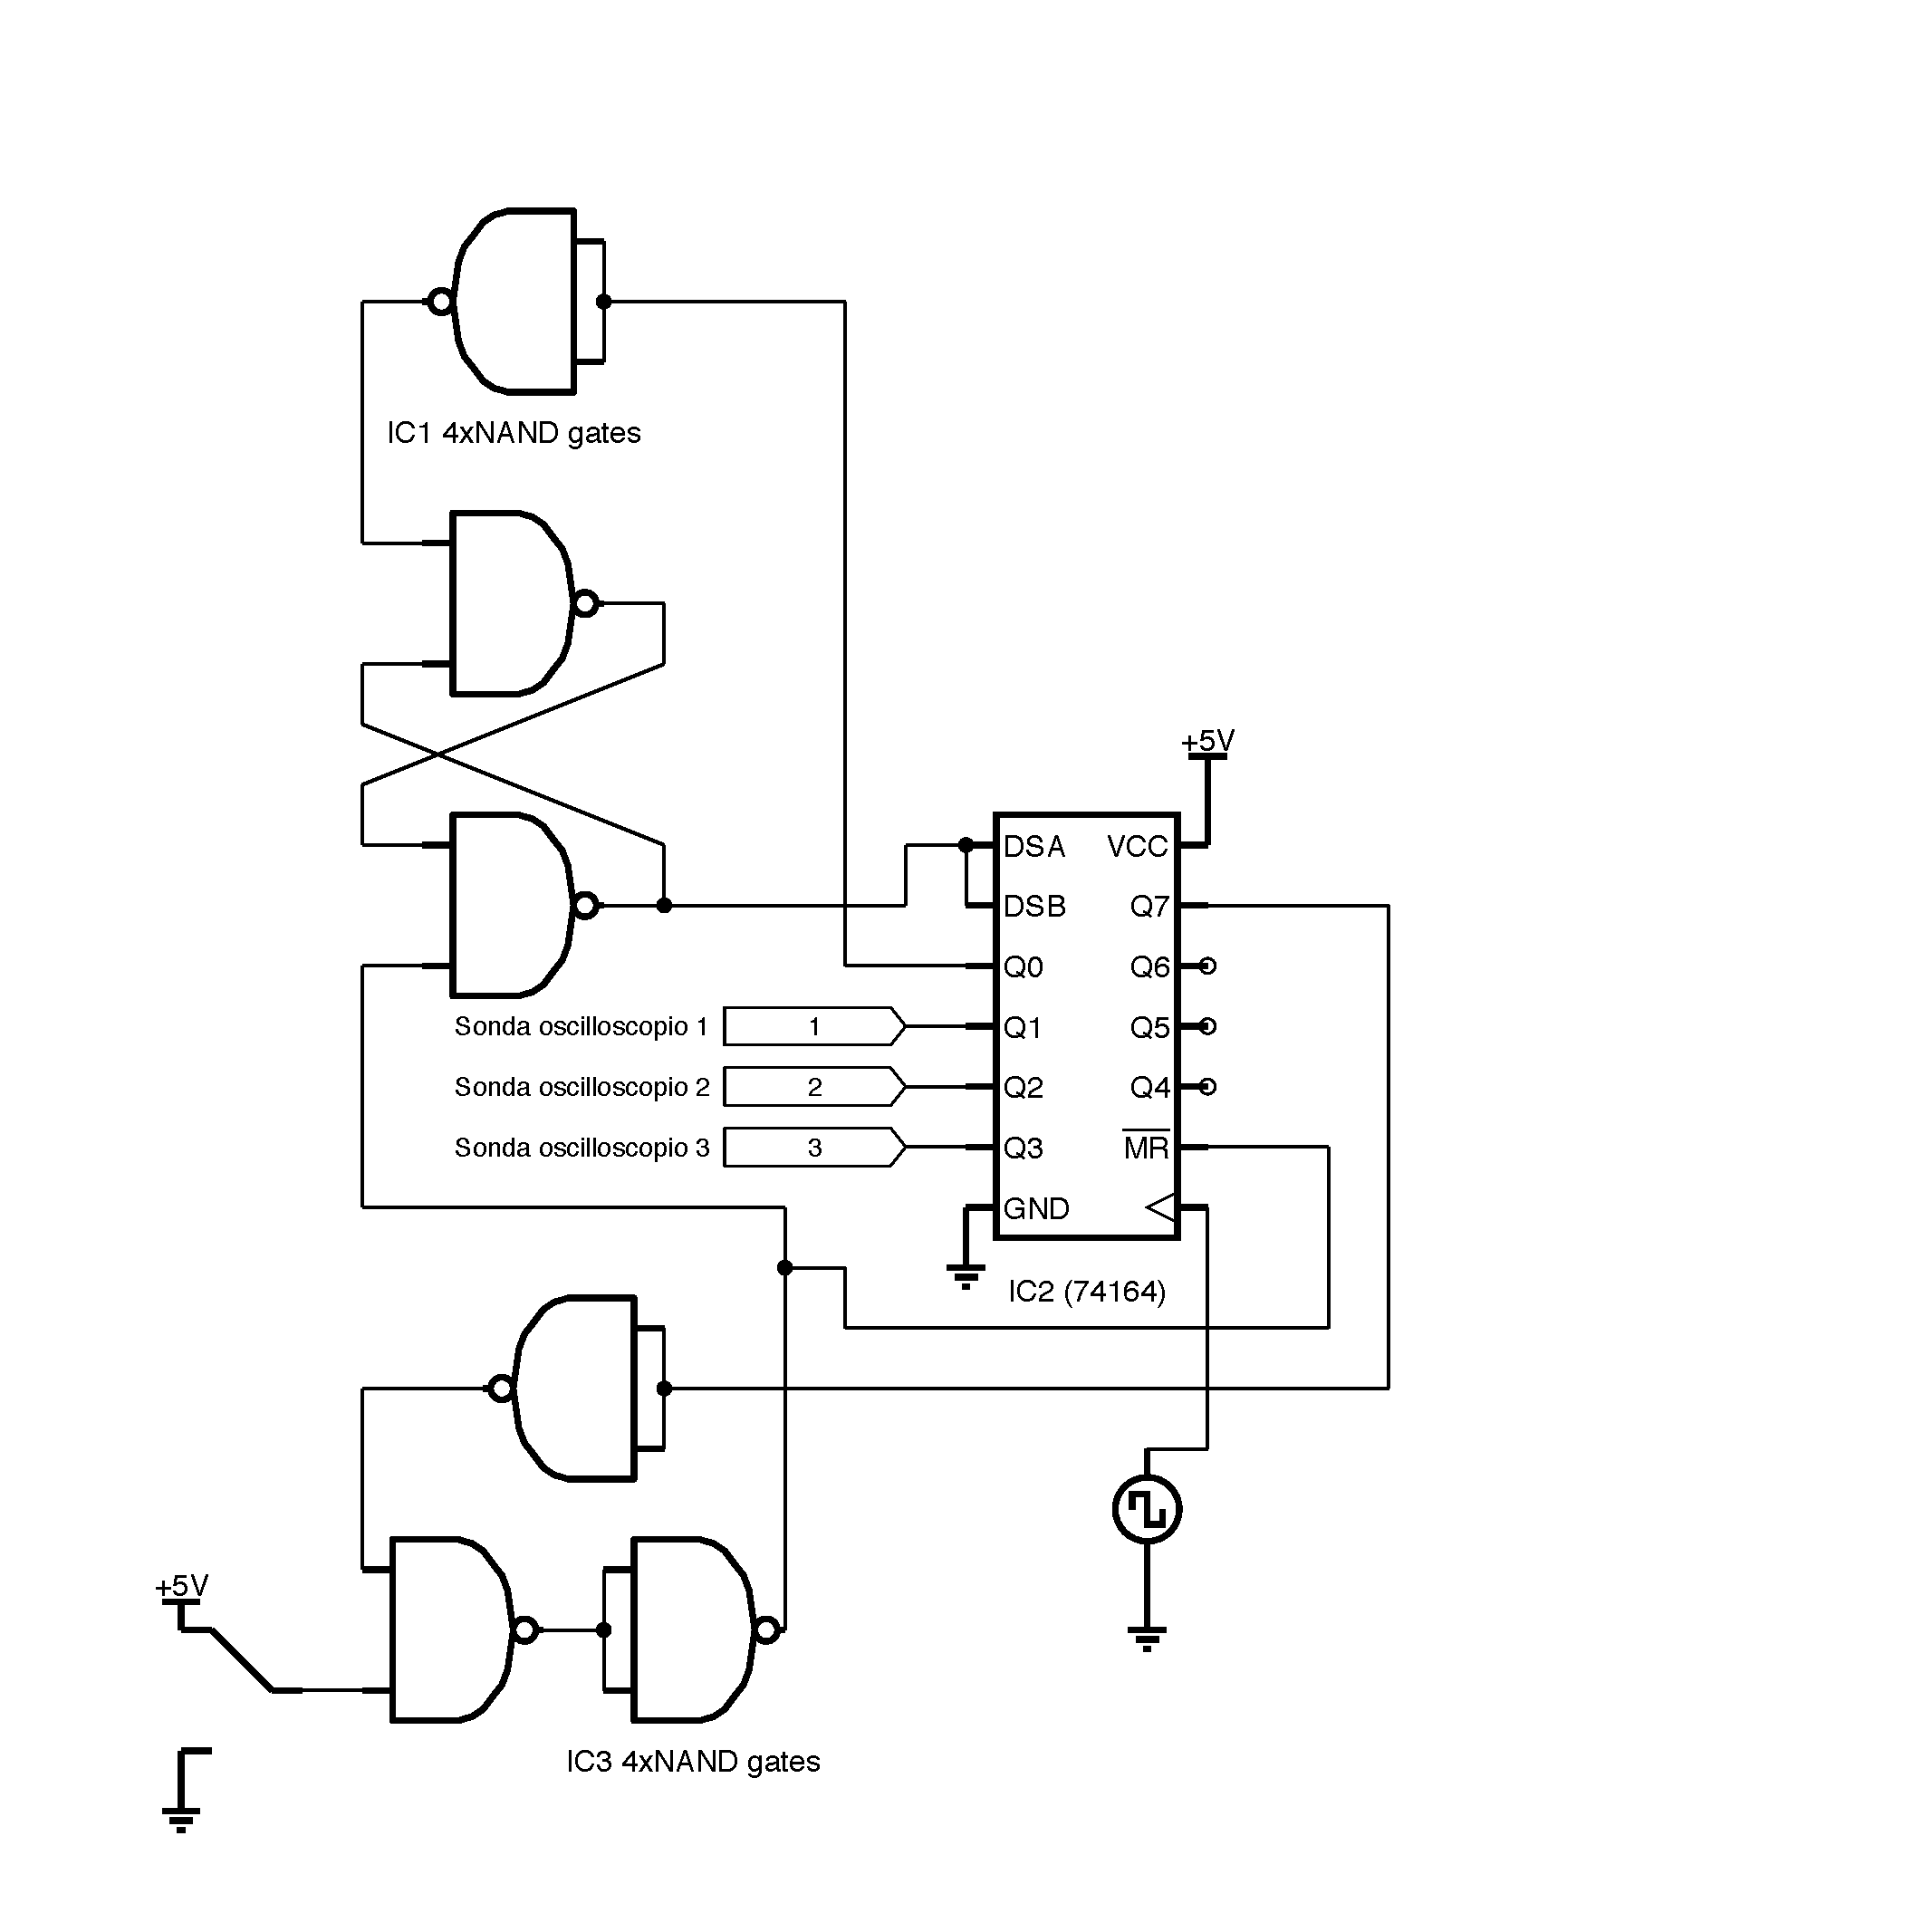
\includegraphics[width=0.50\textwidth]{sch-simulations/digital/output/shift-register.pdf}
\caption{Registro a scorrimento e circuito di controllo}
\label{fig:circuit_shift_register}
\end{center}
\end{figure}


Gli \textit{shift register} (registri a scorrimento) sono un tipo di circuito logico sequenziale sfruttato principalmente per l'archiviazione di dati digitali o per la lettura in parallelo di dati trasferiti in modalità seriale. Il registro utilizzato in laboratorio è realizzato mediante un gruppo di \textit{master-slave flip-flop} collegati in catena in modo che l'output di ogni blocco costituisca l'input del successivo. Tutti i flip-flop sono controllati da un segnale di clock e da un segnale di reset comune.
Ad ogni fronte di salita del clock (il registro utilizzato in laboratorio è del tipo \textit{positive-edge}) lo stato di ogni flip-flop viene trasferito al successivo, mentre il primo della catena viene inizializzato utilizzando i valori logici presenti agli ingressi A e B del registro. Lo stato di ciascun flip-flop può essere letto in modo asincrono in parallelo utilizzando le uscite {$Q_A$, ... , $Q_G$}. Il dispositivo utilizzato in laboratorio per la realizzazione dell'ADC è un registro ad 8 bit \textit{SN74LS164M} corredato da due circuiti logici ausiliari di controllo realizzati con porte NAND:
\begin{itemize}
    \item Il primo (quello che nello schema in figura \ref{fig:circuit_shift_register} è realizzato con l'integrato IC1) controlla l'inizializzazione del registro: quando il segnale di reset passa allo stato basso un flip-flop SR inizializza gli ingressi A e B del registro allo stato alto e attende il primo fronte di salita del clock che fa scorrere il registro di una posizione, a quel punto lo stato alto viene trasferito all'uscita $Q_0$ (o $Q_A$) il cui complemento logico esegue il reset del flip-flop riportando gli ingressi A e B al valore basso. 
    \item Il secondo (quello che nello schema in figura \ref{fig:circuit_shift_register} è realizzato con l'integrato IC3) è invece responsabile dell'operazione di RESET: quando il bit 1 con cui era stato inizializzato il registro raggiunge l'ultima uscita $Q_7$ (o $Q_H$) oppure quando lo switch manuale di reset viene portato allo stato basso, il circuito porta il segnale di clear globale allo stato basso, effettuando così il reset di tutti i circuiti logici.
\end{itemize}

La figura seguente mostra la verifica effettuata in laboratorio sul corretto funzionamento di questo circuito: il canale 4 dell'oscilloscopio acquisisce il segnale di trigger (realizzato con il generatore di funzioni utilizzando un'onda quadra oscillante tra 0 V e 5 V con frequenza di 5 Hz) mentre i primi tre canali (come segnato nello schema in figura \ref{fig:circuit_shift_register}) sono collegati alle tre uscite del registro successive alla prima. Dopo aver effettuato il reset osserviamo che il registro viene inizializzato dal circuito di controllo con un solo bit allo stato alto e questo bit viene fatto scorrere fino alla fine, quando avverrà un nuovo reset. 


\begin{figure}[H]%[!ht]
\begin{center}
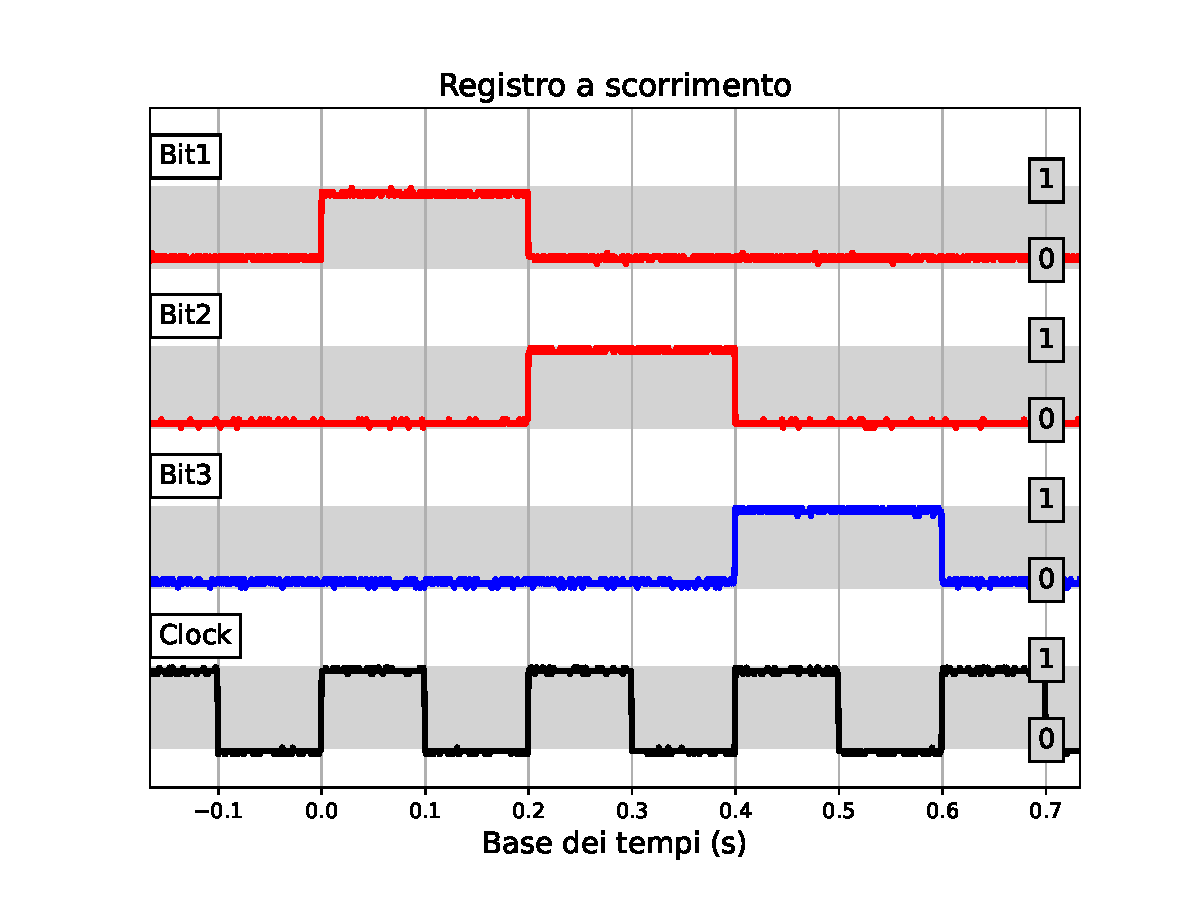
\includegraphics[trim = {0 0 0 0}, clip, width=0.50\textwidth]{analysis/output/reg_test.pdf}
\caption{BIT con transistor}
\label{fig:BIT_with_transistor}
\end{center}
\end{figure}

\subsection{Verifica del circuito di pilotaggio del DAC (J-K) e dello stadio analogico}
Descriviamo e verifichiamo ora il sottocircuito successivo che consente il funzionamento dell'ADC: il circuito di pilotaggio del DAC realizzato con flip-flop di tipo J-K. L'obiettivo di questo circuito è di effettuare il confronto del valore di ogni bit con la tensione da misurare mediante il pilotaggio del DAC, realizzando il processo di approssimazioni successive. 

\begin{figure}[H]%[!ht]
\begin{center}
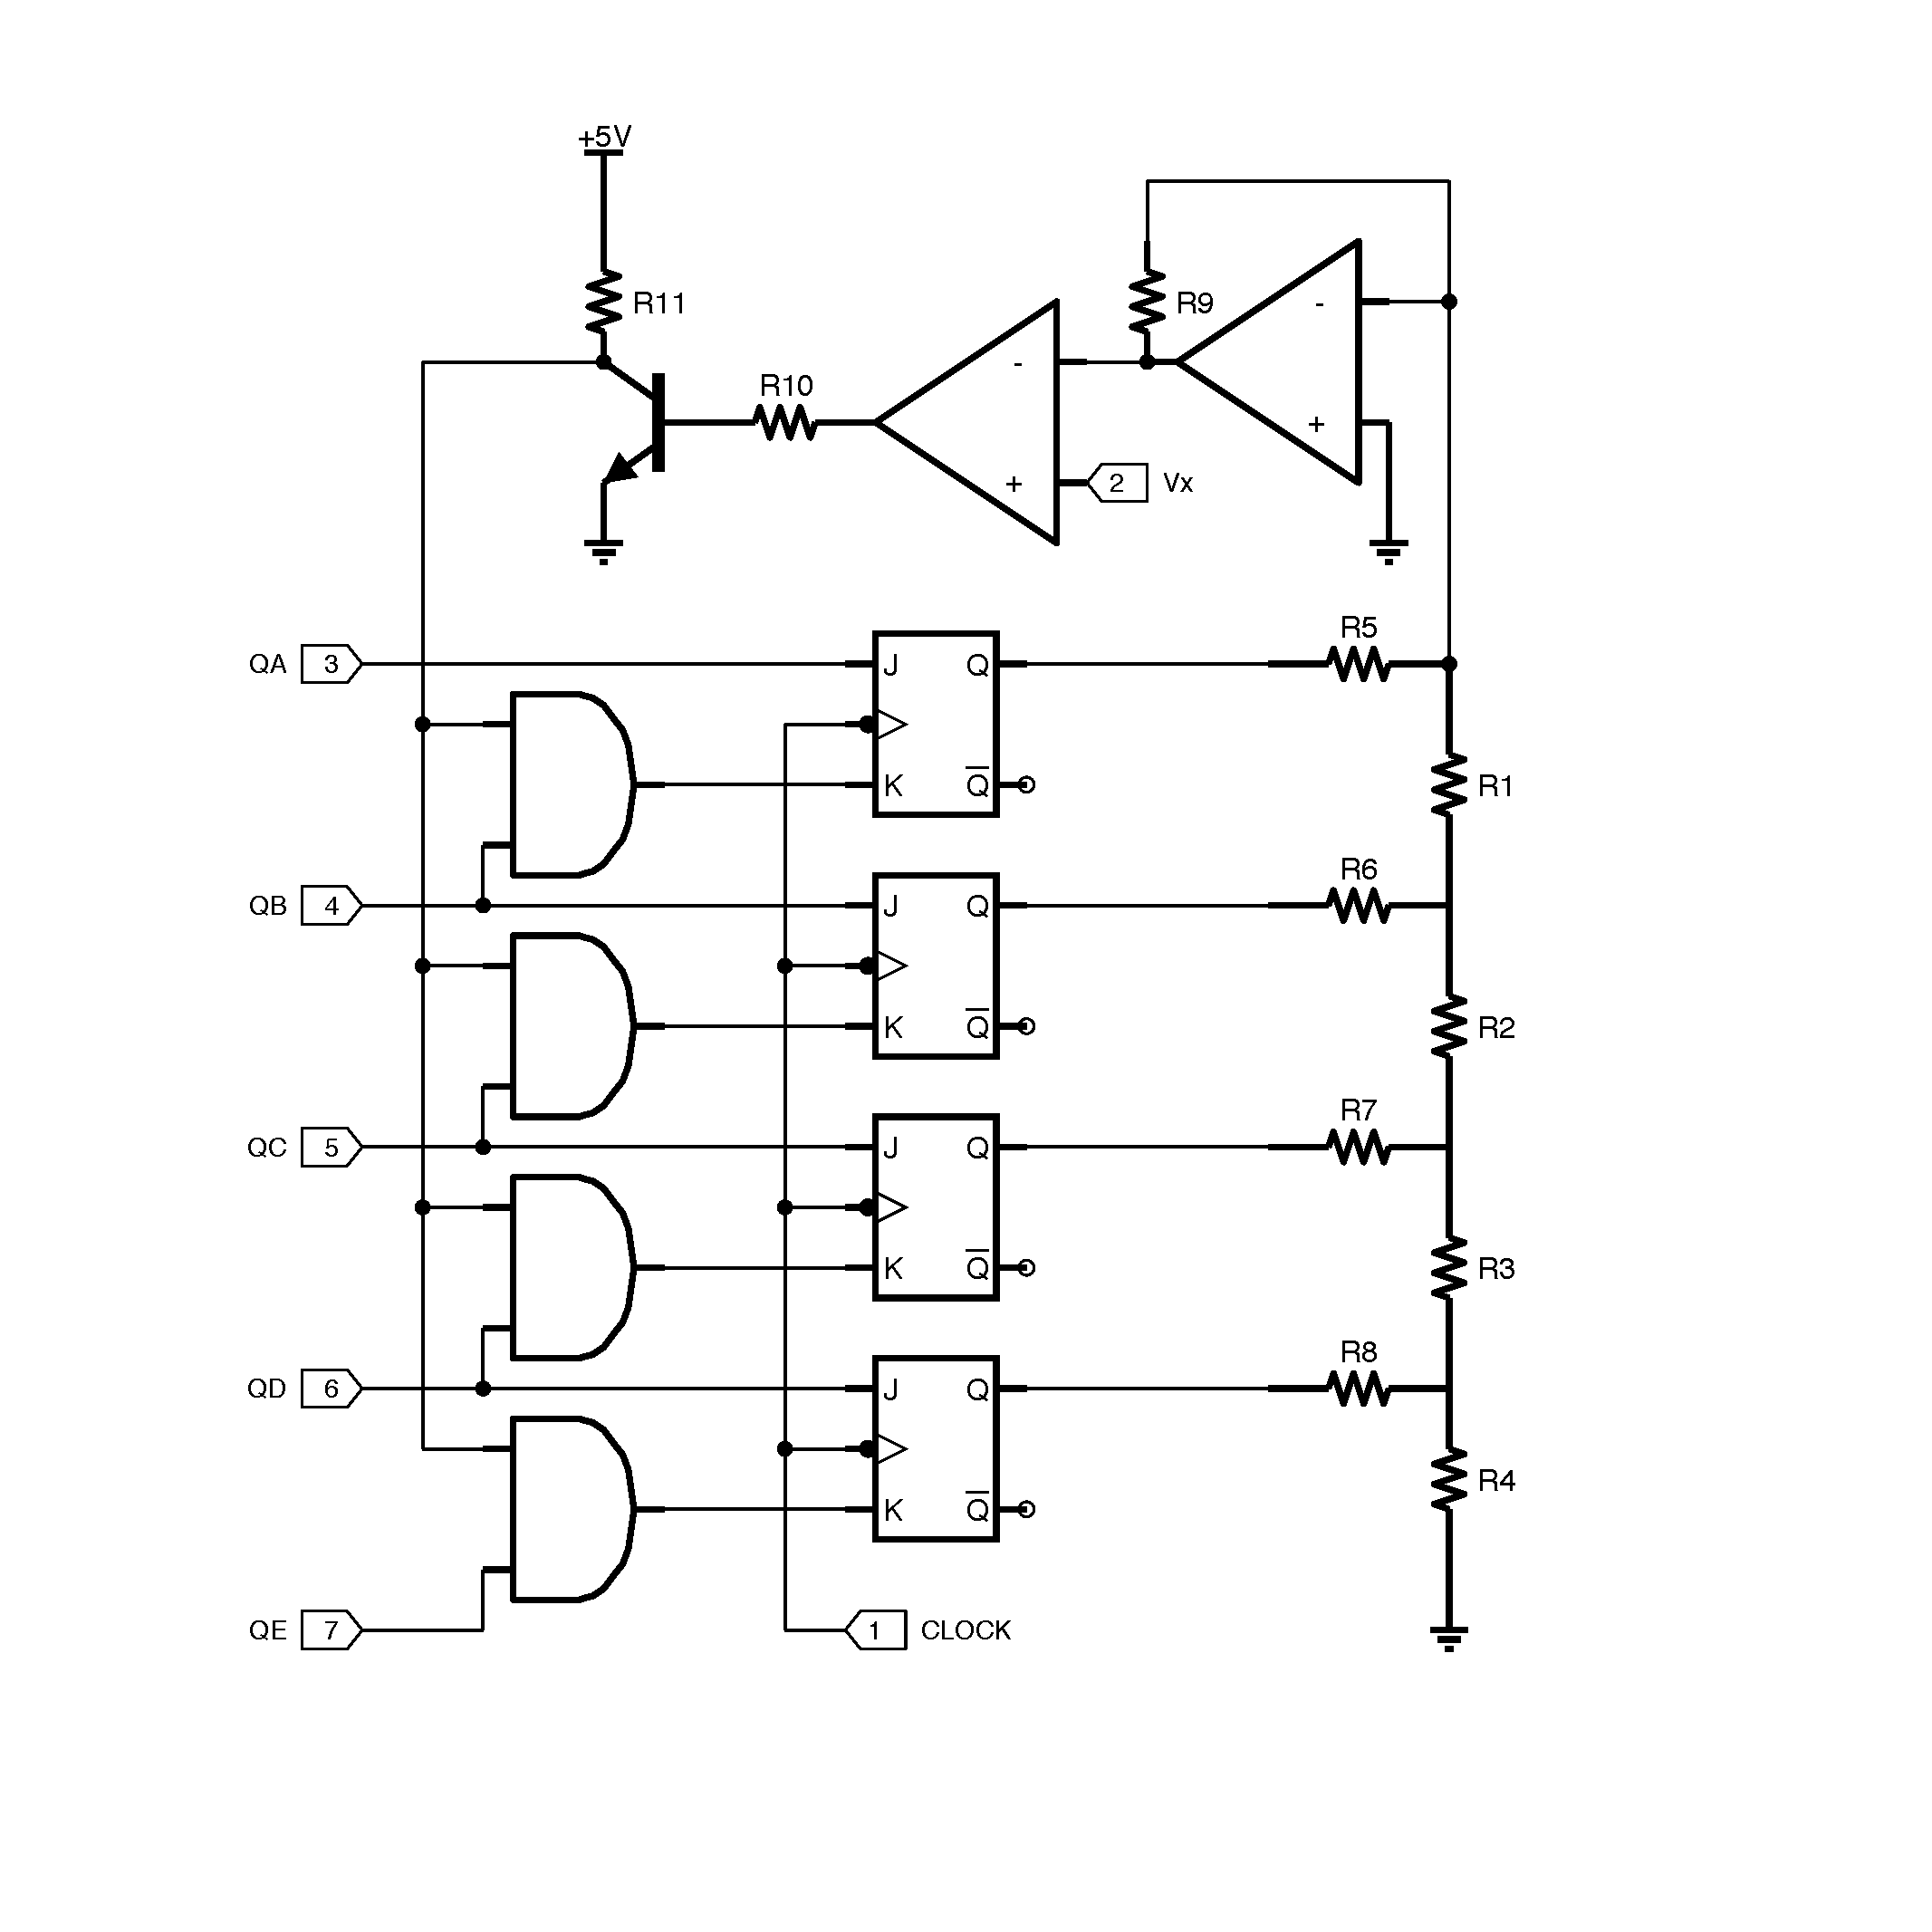
\includegraphics[width=0.48\textwidth]{sch-simulations/digital/output/DAC.pdf}
\caption{Circuito di controllo del DAC con flip-flop J-K e sezione analogica dell'ADC.}
\label{fig:circuit_DAC}
\end{center}
\end{figure}


Il funzionamento è il seguente: ogni uscita del registro di scorrimento attiva il J di ciascun flip-flop e, con l'esclusione della prima, attiva il K del flip-flop precedente. Mentre però l'operazione di set J è sempre effettuata, l'operazione di reset K è effettuata solo se il complemento logico dell'uscita del comparatore è alto, perché ogni ingresso K non è direttamente collegato al registro, ma bensì attraverso una porta AND con il segnale logico proveniente dal comparatore. Il risultato è che ogni bit viene attivato, ma viene disattivato solo in base all'operazione di confronto, quindi al termine del ciclo di conversione lo stato delle uscite dei J-K costituirà la rappresentazione binaria del segnale quantizzato. 

La verifica in laboratorio si è svolta dapprima collegando le 4 uscite dei J-K ai 4 canali dell'oscilloscopio e forzando al livello basso il complemento logico dell'uscita del comparatore (si veda la figura \ref{fig:cumulative_BIT}), in questo caso, come atteso osserviamo che in un ciclo di conversione tutti i bit vengono attivati e rimangono allo stato alto fino al segnale di reset, che coinvolge anche i J-K.

Nella figura \ref{fig:cumulative_BIT_clk} osserviamo il medesimo scenario di funzionamento, ma questa volta la sonda collegata al canale 4 dell'oscilloscopio è stata collegata al clock e questo ci permette di osservare, per esempio, che la commutazione dei J-K avviene sul fronte di discesa. Per il corretto funzionamento dell'ADC è molto rilevante che le la commutazione del registro avvenga sul fronte di salita del clock, mentre quella dei J-K avvenga sul fronte di discesa, in questo modo quando i flip-flop leggono i loro ingressi J e K il registro li ha già sicuramente portati ad uno stato logico valido.

\begin{figure}[H]%[!ht]
\begin{center}
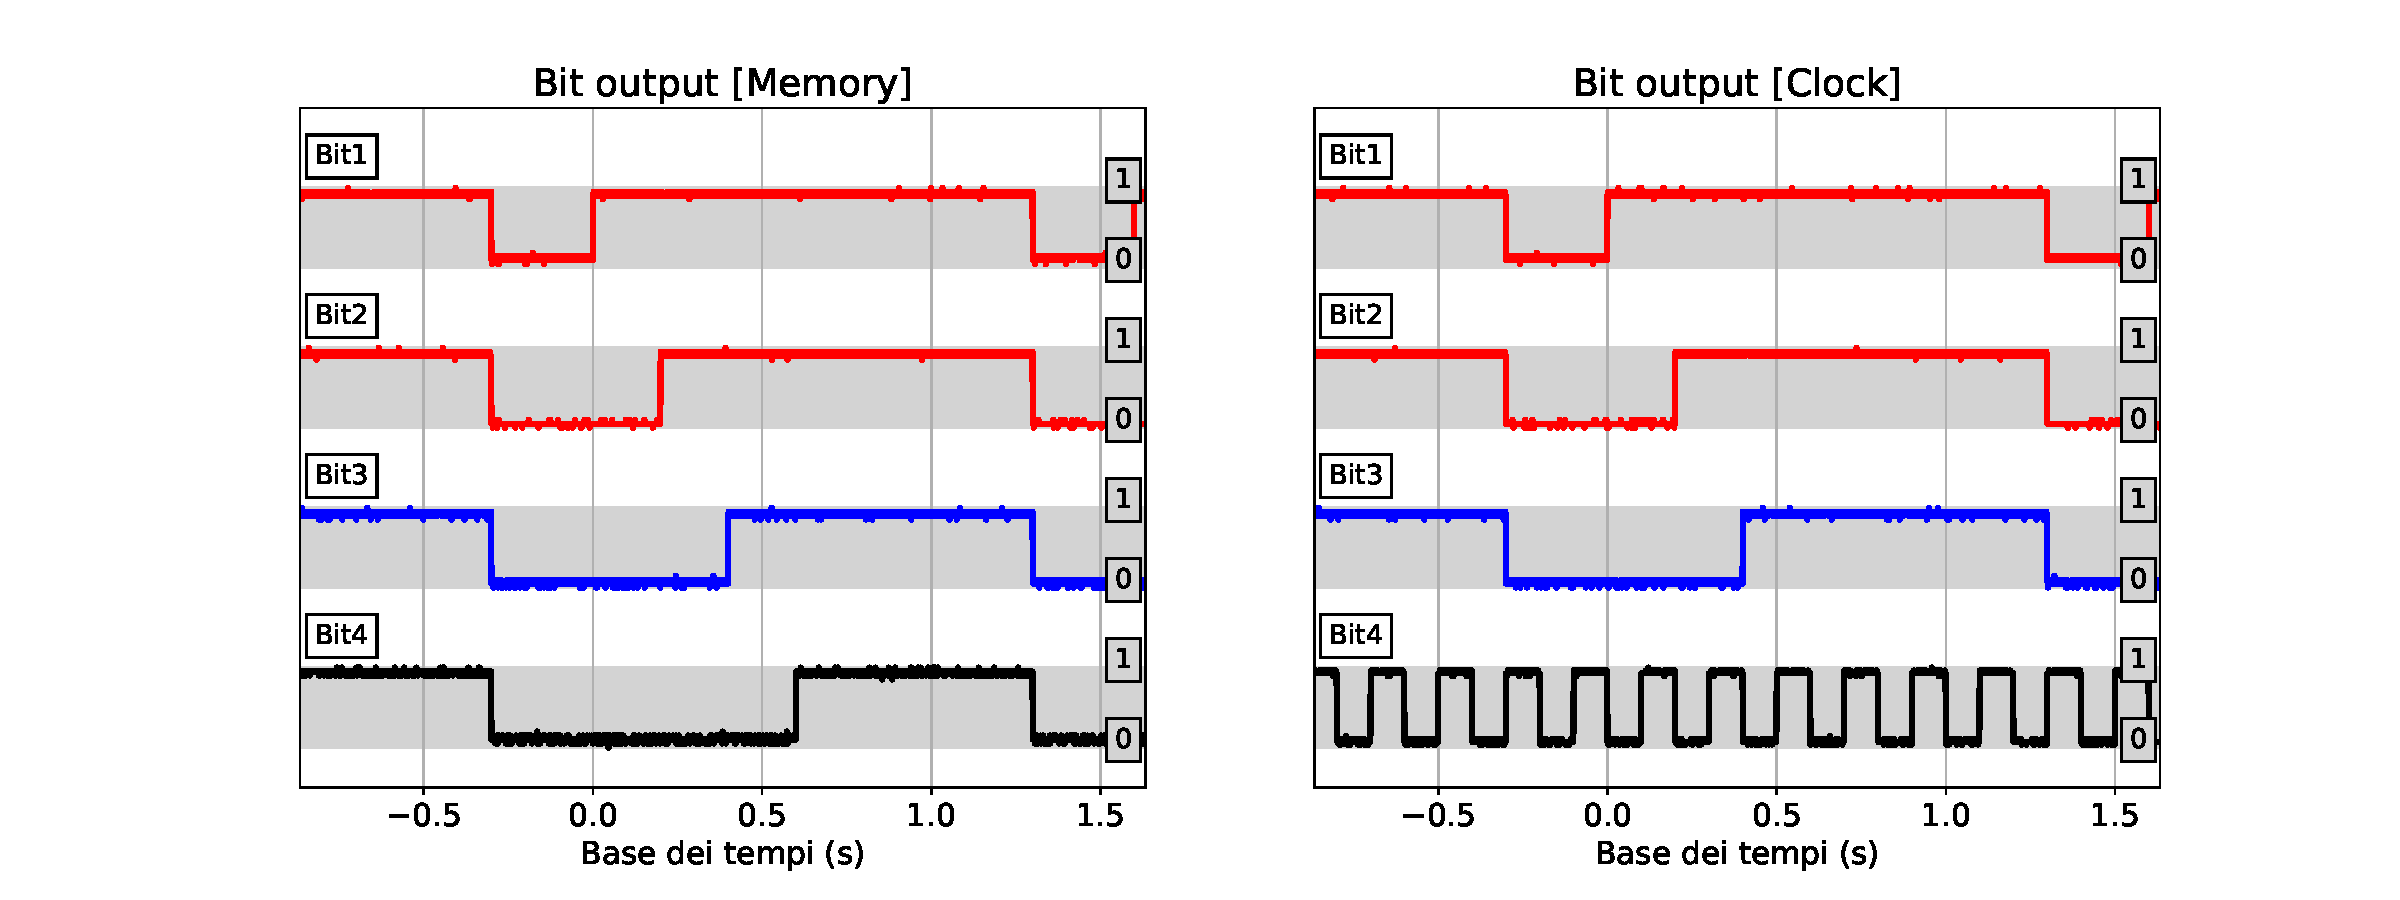
\includegraphics[trim = {100 0 550 0}, clip, width=0.43\textwidth]{analysis/output/cumulative_BIT.pdf}
\caption{Uscite dei flip-flop J-K quando il complemento logico del comparatore è allo stato basso}
\label{fig:cumulative_BIT}
\end{center}
\end{figure}

\vspace{-10mm}

\begin{figure}[H]%[!ht]
\begin{center}
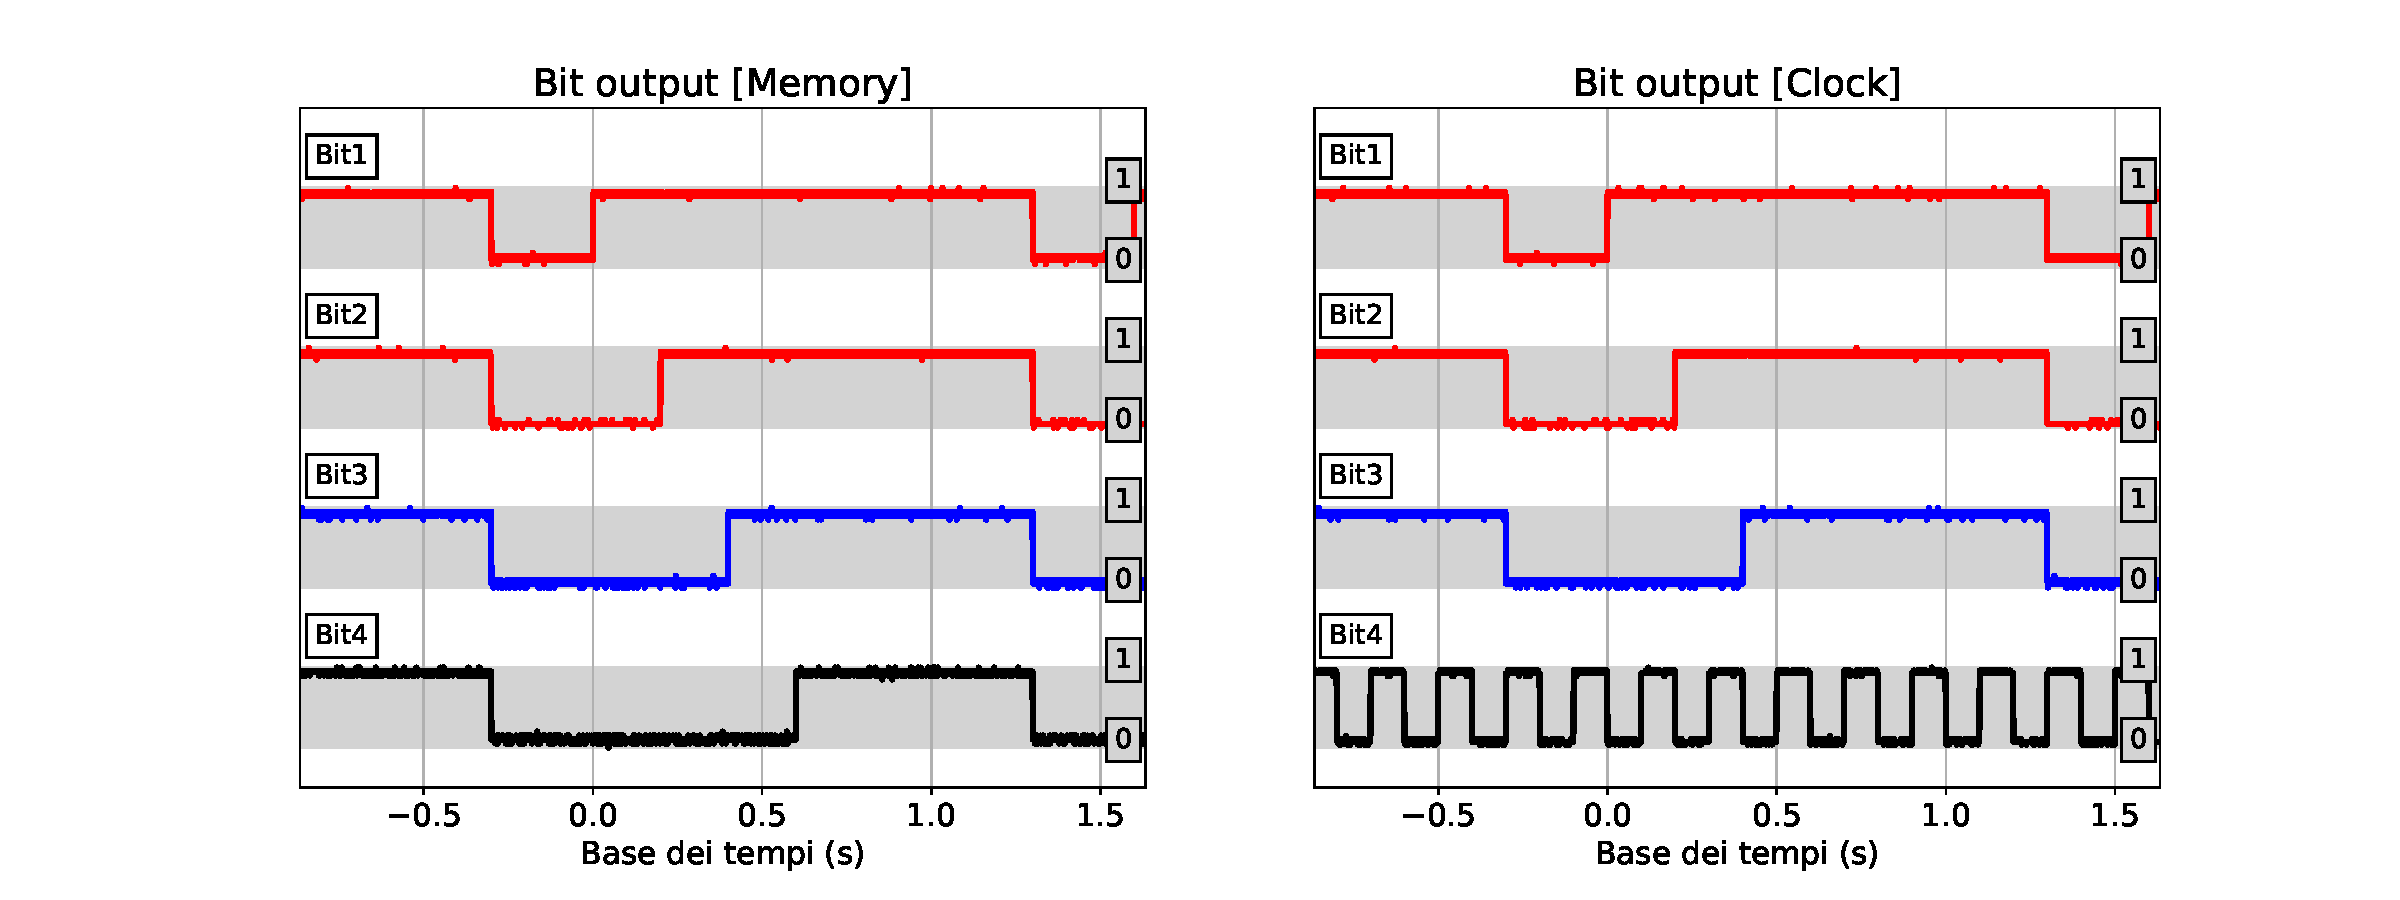
\includegraphics[trim = {600 0 100 0}, clip, width=0.39\textwidth]{analysis/output/cumulative_BIT.pdf}
\label{fig:cumulative_BIT_clk}
\end{center}
\end{figure}

\vspace{-7mm}

Nella figura seguente si osserva la medesima misura effettuata però forzando il complemento logico dell'uscita del comparatore allo stato alto. Le uscte delle porte AND che controllano gli ingressi K potranno quindi raggiungere lo stato alto e ogni bit verrà resettato sul fronte di discesa del \textit{clock} in cui viene settato il bit successivo.

\begin{figure}[H]%[!ht]
\begin{center}
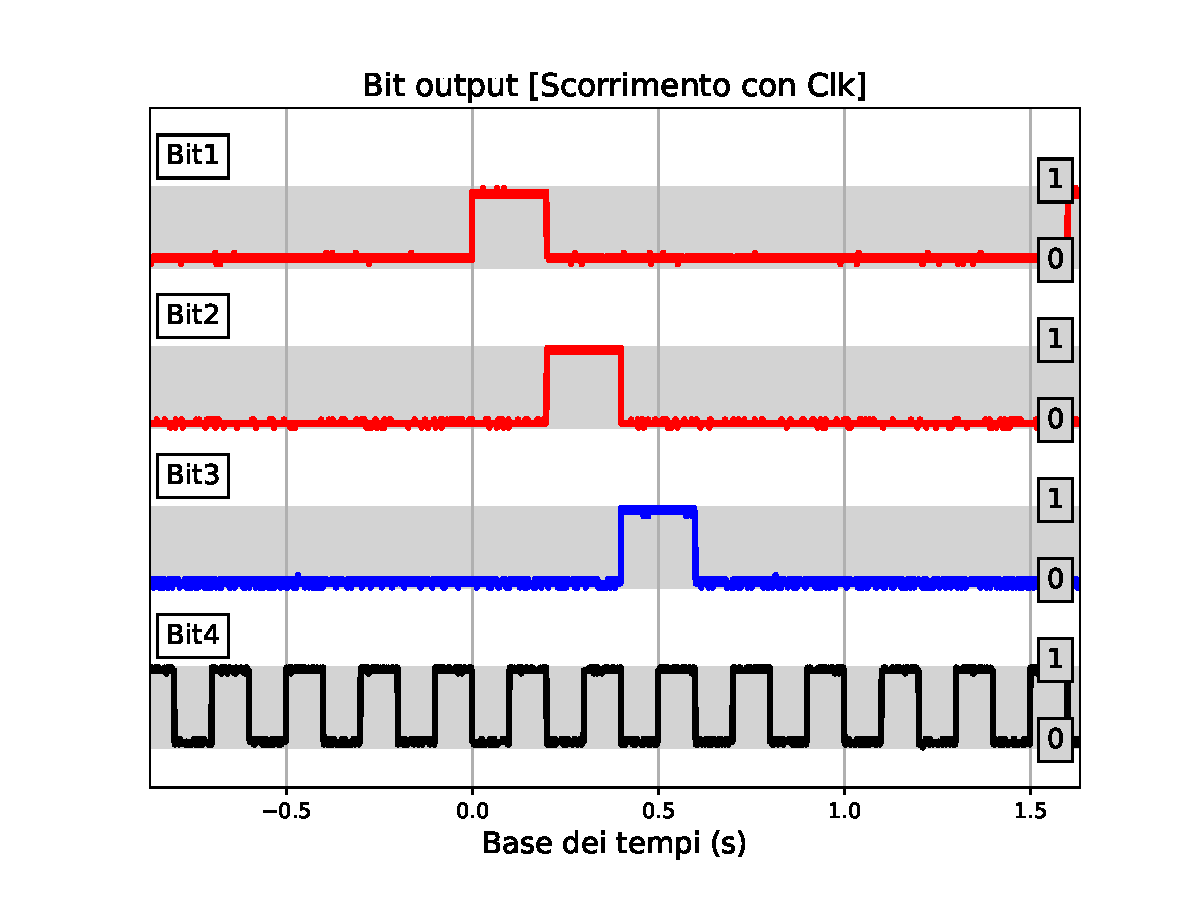
\includegraphics[width=0.48\textwidth]{analysis/output/BIT-shift-clk.pdf}
\label{fig:BIT_shift_clk}
\end{center}
\end{figure}

Per realizzare l'acquisizione seguente sono state invece collegati i primi tre canali dell'oscilloscopio alle uscite dei J-K, ma l'ultimo canale è stato collegato alla base del transistor di interfaccia del comparatore, quindi mostra esattamente il risultato logico dell'operazione di confronto. Osserviamo che quando l'operazione di confronto restituisce 0 (uscita del DAC più alta del segnale in ingresso) le porte AND possono attivarsi e i bit vengono man mano resettati, mentre quando l'operazione di confronto restituisce 1 (uscita del DAC più bassa del segnale in ingresso) i bit rimangono attivi quando la conversione giunge al termine.

\begin{figure}[H]%[!ht]
\begin{center}
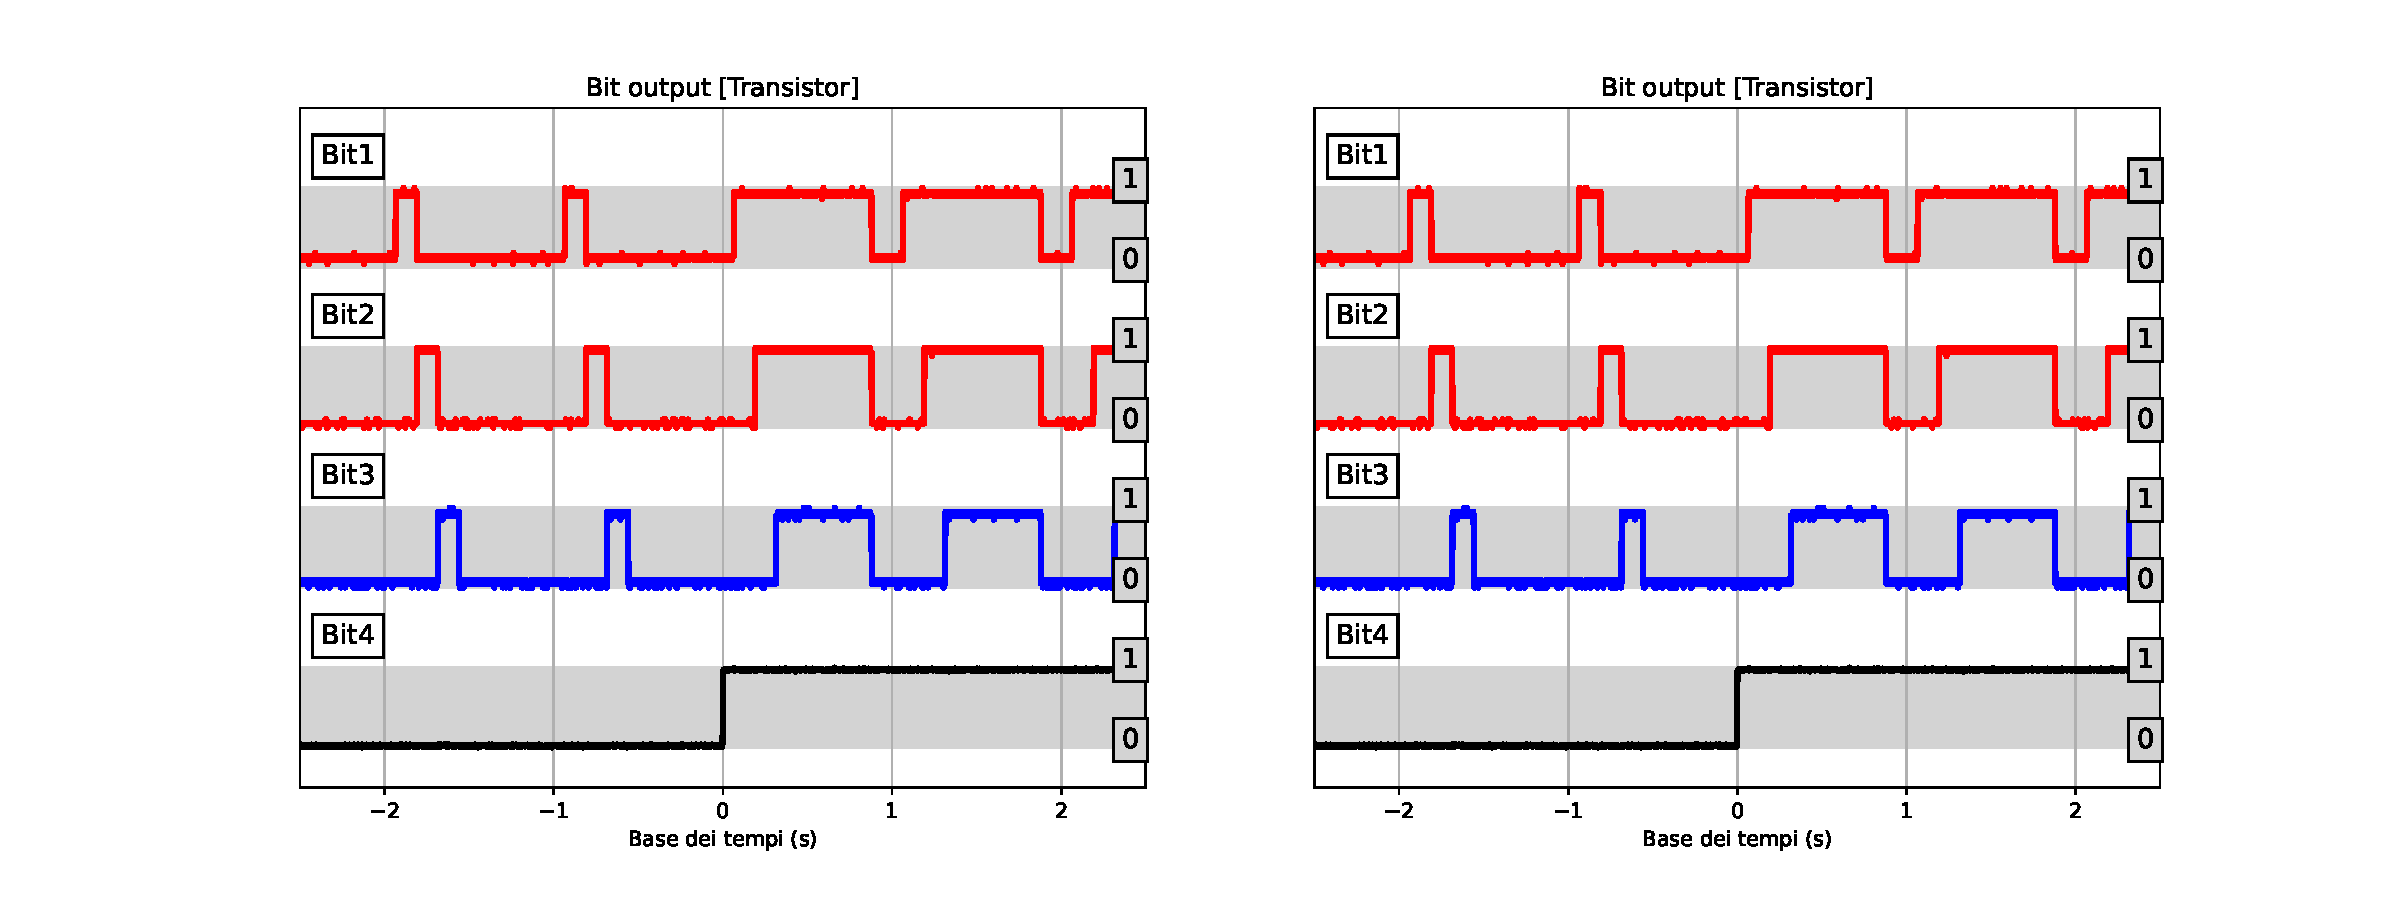
\includegraphics[trim = {570 0 0 0}, clip, width=0.50\textwidth]{analysis/output/cumulative_BIT_with_transistor.pdf}
\caption{Uscite dei J-K sui primi tre ingressi dell'oscilloscopio, sul 4 il livello logico dell'uscita del comparatore}
\label{fig:BIT_with_transistor}
\end{center}
\end{figure}

\subsection{Convertitore digitale-analogico}
Il confronto tra il valore logico rappresentato dalle uscite dei flip-flop J-K e il segnale analogico in ingresso è possibile solo grazie ad un DAC di tipo R-2R pilotato da tali uscite. Il DAC è realizzato mediante resistori discreti dei valori riportati a seguire che realizzano una rete che alimenta l'ingresso invertente di un amplificatore operazionale retroazionato a guadagno unitario (LM741). L'uscita di tale amplificatore operazionale controlla l'ingresso invertente di un secondo componente identico che lavora però in configurazione ad anello aperto, realizzando così il comparatore vero e proprio, dal momento che il suo ingresso non invertente costituisce l'ingresso analogico dell'ADC. Come anticipato, si rende necessaria l'introduzione di un transistor di interfaccia con tre funzioni:
\begin{itemize}
    \item Adatta i livelli di tensione $\pm$ 15 V ai livelli logici TTL 0V - 5V
    \item Effettua un'operazione di "NOT" logico
    \item Grazie all'amplificazione dovuta alla configurazione ad emettitore comune rende più ripido i fronti di commutazione dell'uscita del comparatore, consentendo all'ADC di lavorare a frequenze più elevate.
\end{itemize}




\begin{table}[H]
\begin{center}
\caption{Resistori utilizzati per il DAC}
\begin{tabular}{c|c}
Nome in fig.\ref{fig:nyquist_mcu_cumulative} & R [k$\Omega $] \\ \hline
R1  & $1.00 \pm 0.01$ \\
R2  & $1.00 \pm 0.01$ \\
R3  & $1.00 \pm 0.01$ \\
R4  & $2.01 \pm 0.02$ \\
R5  & $1.94 \pm 0.02$ \\
R6  & $1.94 \pm 0.02$ \\
R7  & $2.01 \pm 0.02$ \\
R8  & $1.99 \pm 0.02$ \\
\label{tab:resistori_dac}
\end{tabular}
\end{center}
\end{table}


\subsection{Caratteristica di trasferimento del transistor di interfaccia}
Testo

\begin{figure}[H]%[!ht]
\begin{center}
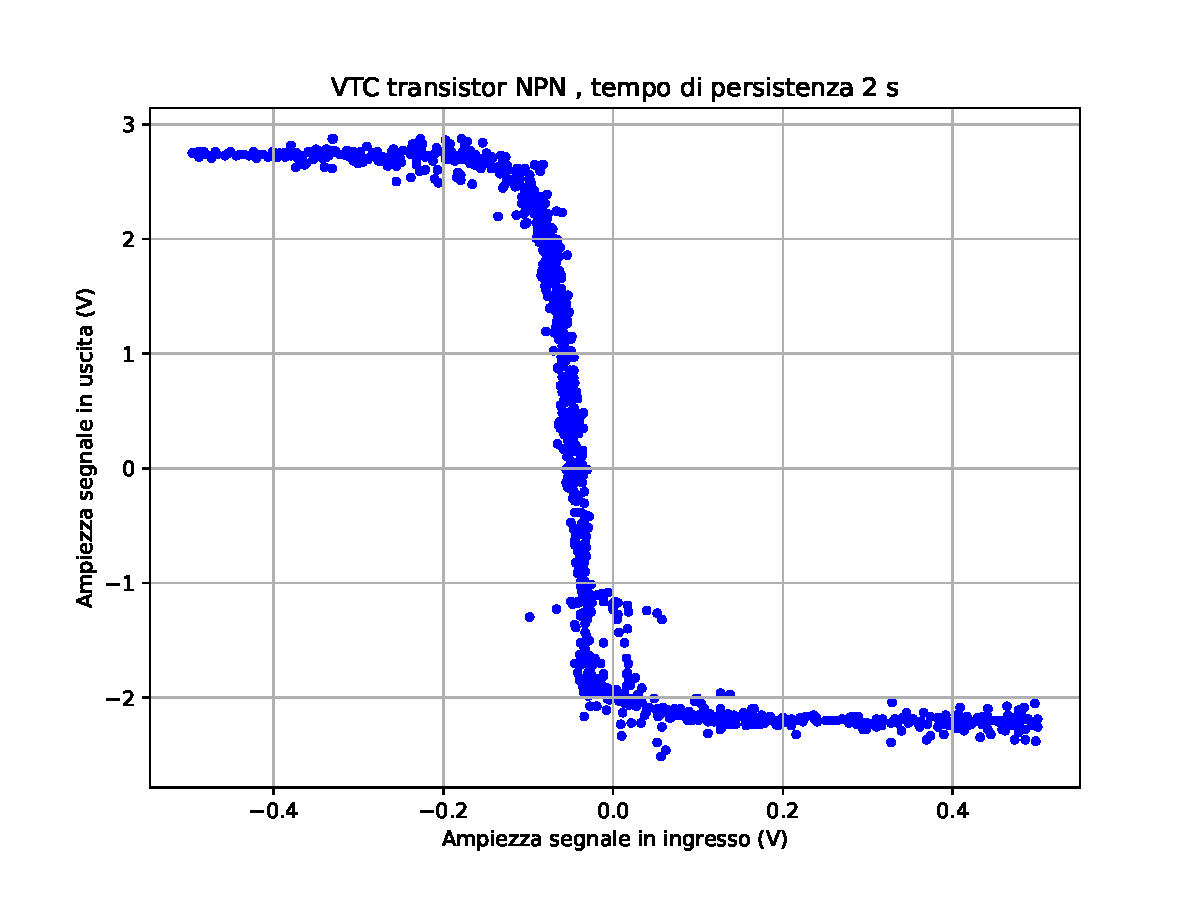
\includegraphics[width=0.45\textwidth]{analysis/output/NPN-XY.pdf}
\caption{Caratteristica di trasferimento in tensione base-collettore del transistor di interfaccia.}
\label{fig:inverter_ring_xy}
\end{center}
\end{figure}


\subsection{Caratteristiche del segnale di \textit{clear}}
Testo

\begin{figure}[H]%[!ht]
\begin{center}
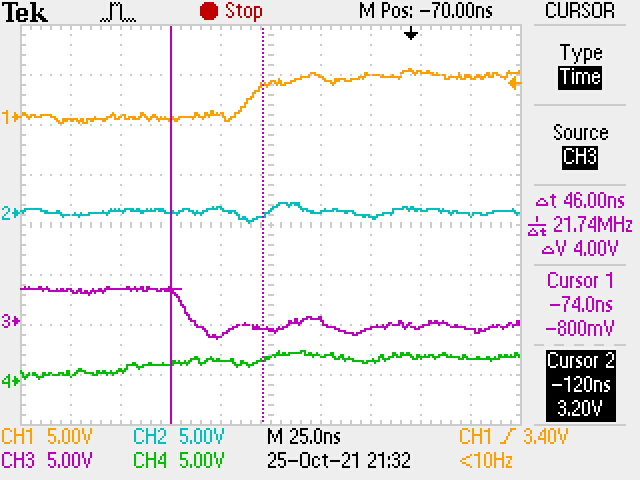
\includegraphics[width=0.45\textwidth]{data-source/25-10-21/DeltaT-clear.JPG}
\caption{Ritardo di propagazione attraverso i circuiti logici di U8 del segnale di clear}
\label{fig:inverter_ring_xy}
\end{center}
\end{figure}

%%%%%%%%%%%%%%%%%%%%%%%%%%%%%%%%%%%%%%%%%%%%%%%%%%%%%%%%%%%%%

\section{Calibrazione del DAC}

\begin{figure}[t]%[t]
\centering
\begin{center}
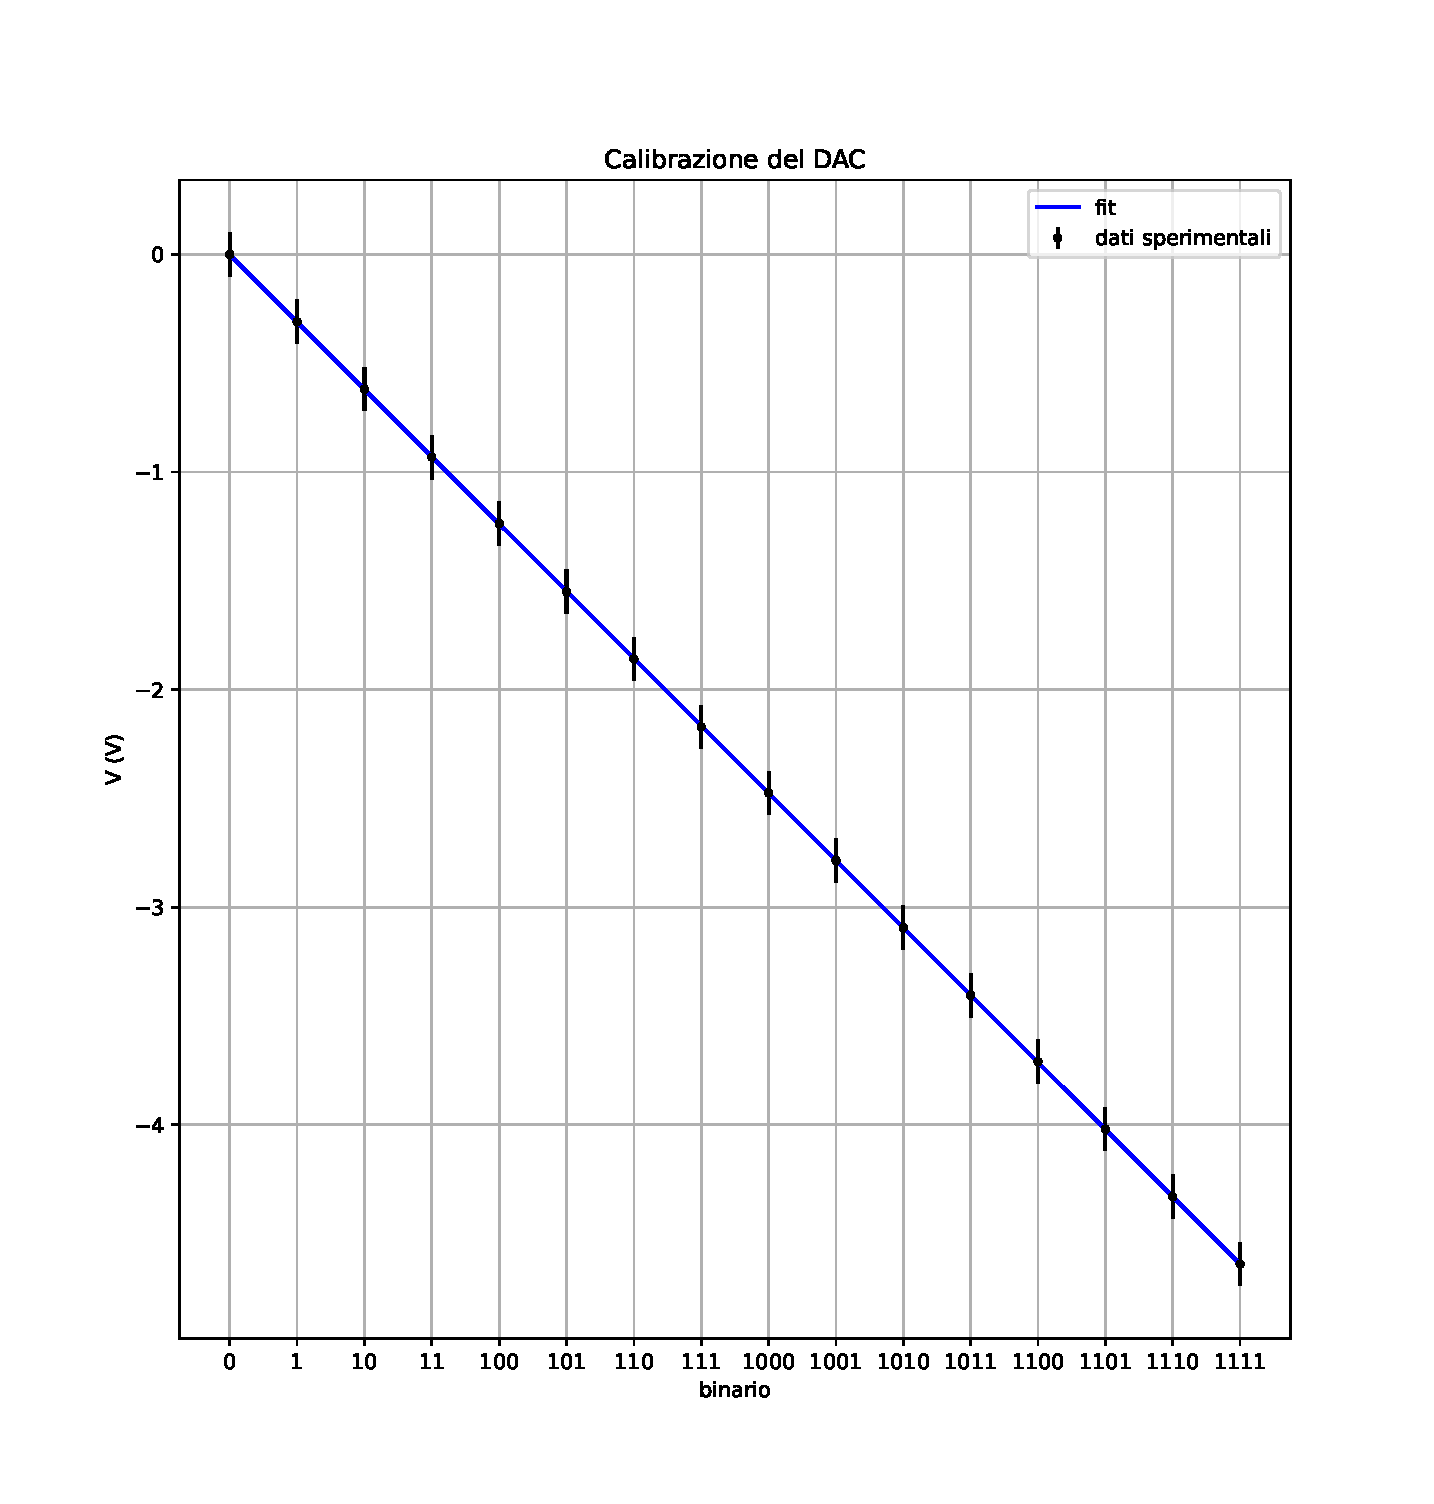
\includegraphics[width=0.51\textwidth]{analysis/output/calibrazione_dac.pdf}
\end{center}
\caption{Retta di calibrazione del DAC, i punti corrispondono alle tensioni misurate all'uscita quando i bit di ingresso vengono portati ai livelli logici rappresentati sull'asse orizzontale.}
\label{fig:graph_calibrazione_dac}
\end{figure}

$ m = -0.211 \pm 0.001 $ \\
$ q = -0.01 \pm 0.01 \ V $ \\
$ \chi^{2} = 0.006 $ \\

\ref{tab:calibrazione_dac}

%%%%%%%%%%%%%%%%%%%%%%%%%%%%%%%%%%%%%%%%%%%%%%%%%%%%%%%%%%%%%

\section{Campionamento di tensioni continue e calibrazione dell'ADC}

\begin{figure}[t]%[t]
\centering
\begin{center}
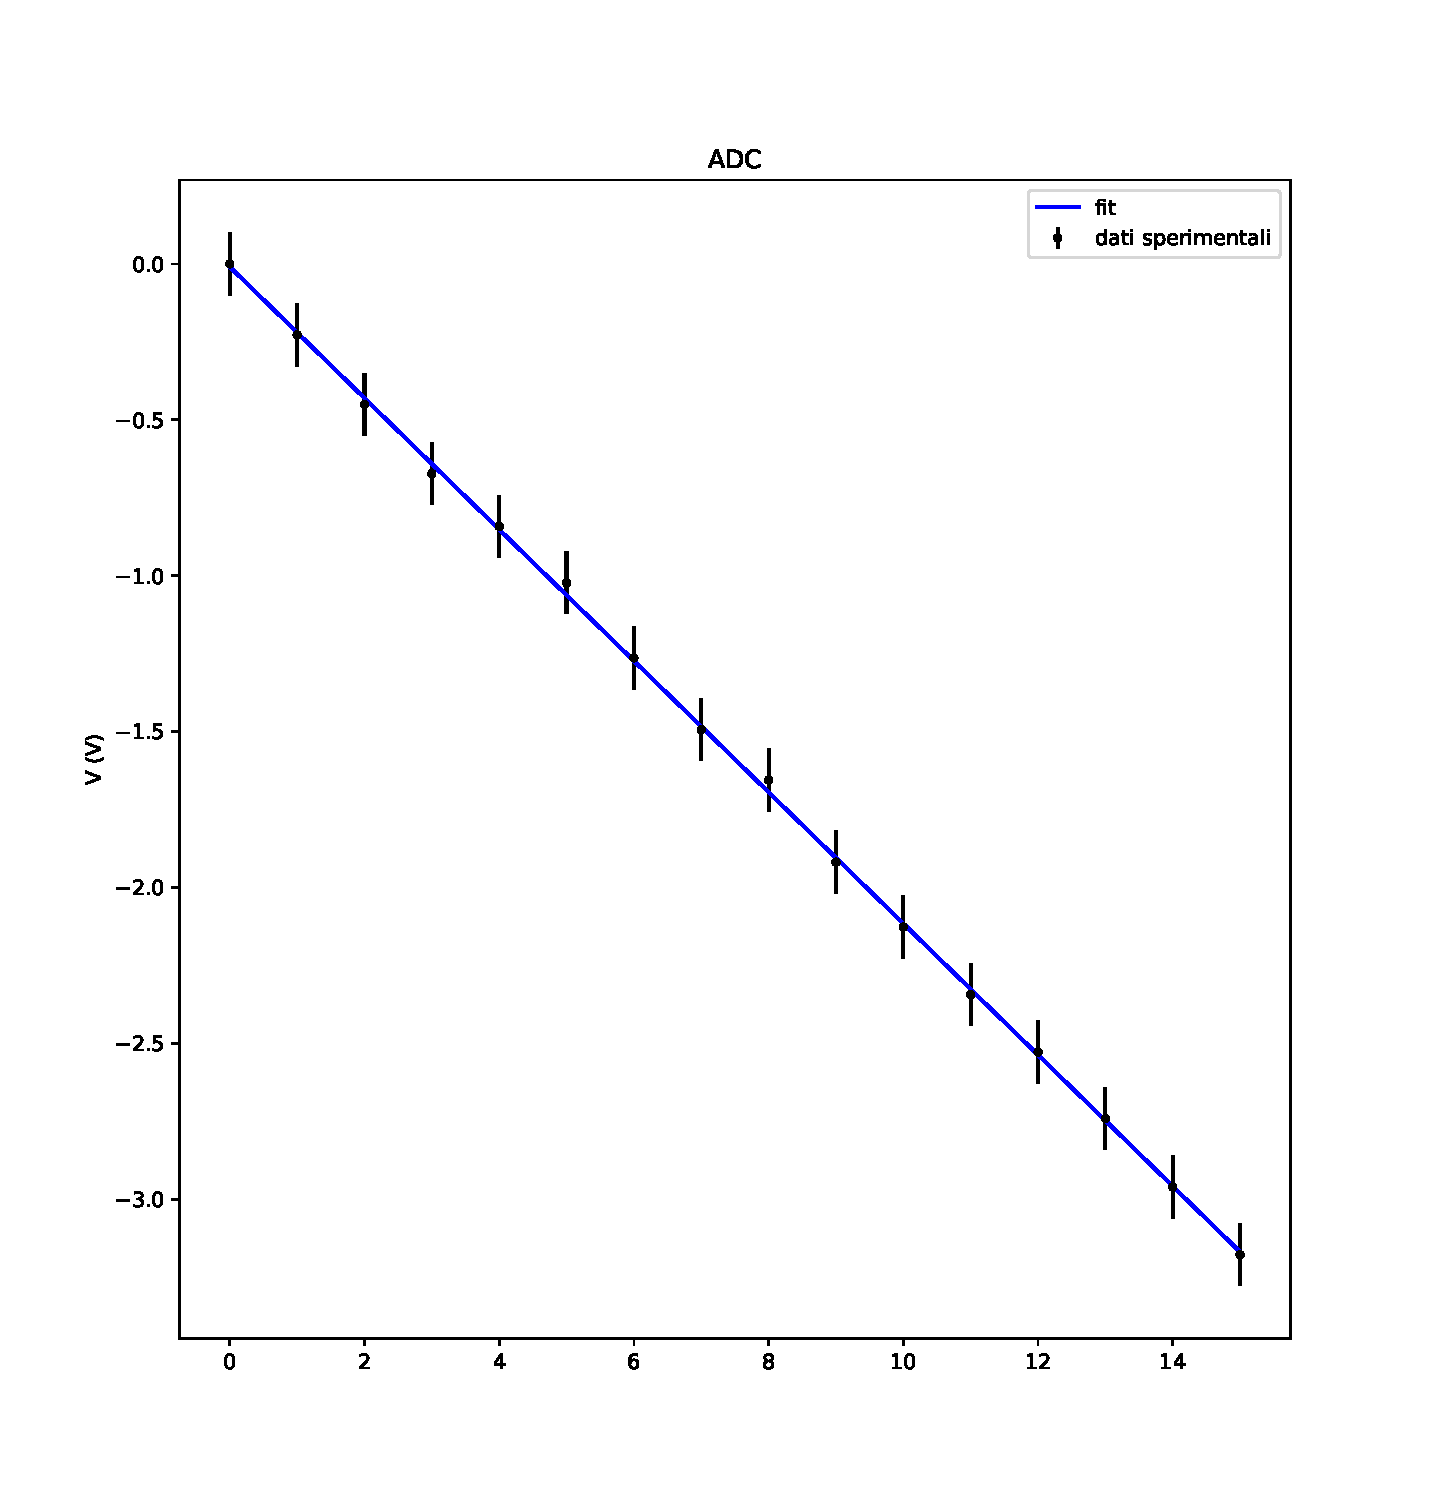
\includegraphics[width=0.51\textwidth]{analysis/output/calibrazione_adc.pdf}
\end{center}
\caption{Retta di calibrazione dell'ADC, i punti corrispondono alle soglie in cui cambia il codice binario restituito facendo variare la tensione in ingresso dal valore più negativo fino a 0 V.}
\label{fig:graph_calibrazione_adc}
\end{figure}

$ m = -0.3092 \pm 0.0001 $ \\
$ q = -0.02 \pm 0.01 \ V$ \\
$ \chi^{2} = 0.57 $ \\

\ref{tab:calibrazione_adc}

\begin{figure*}[t]%[t]
\centering
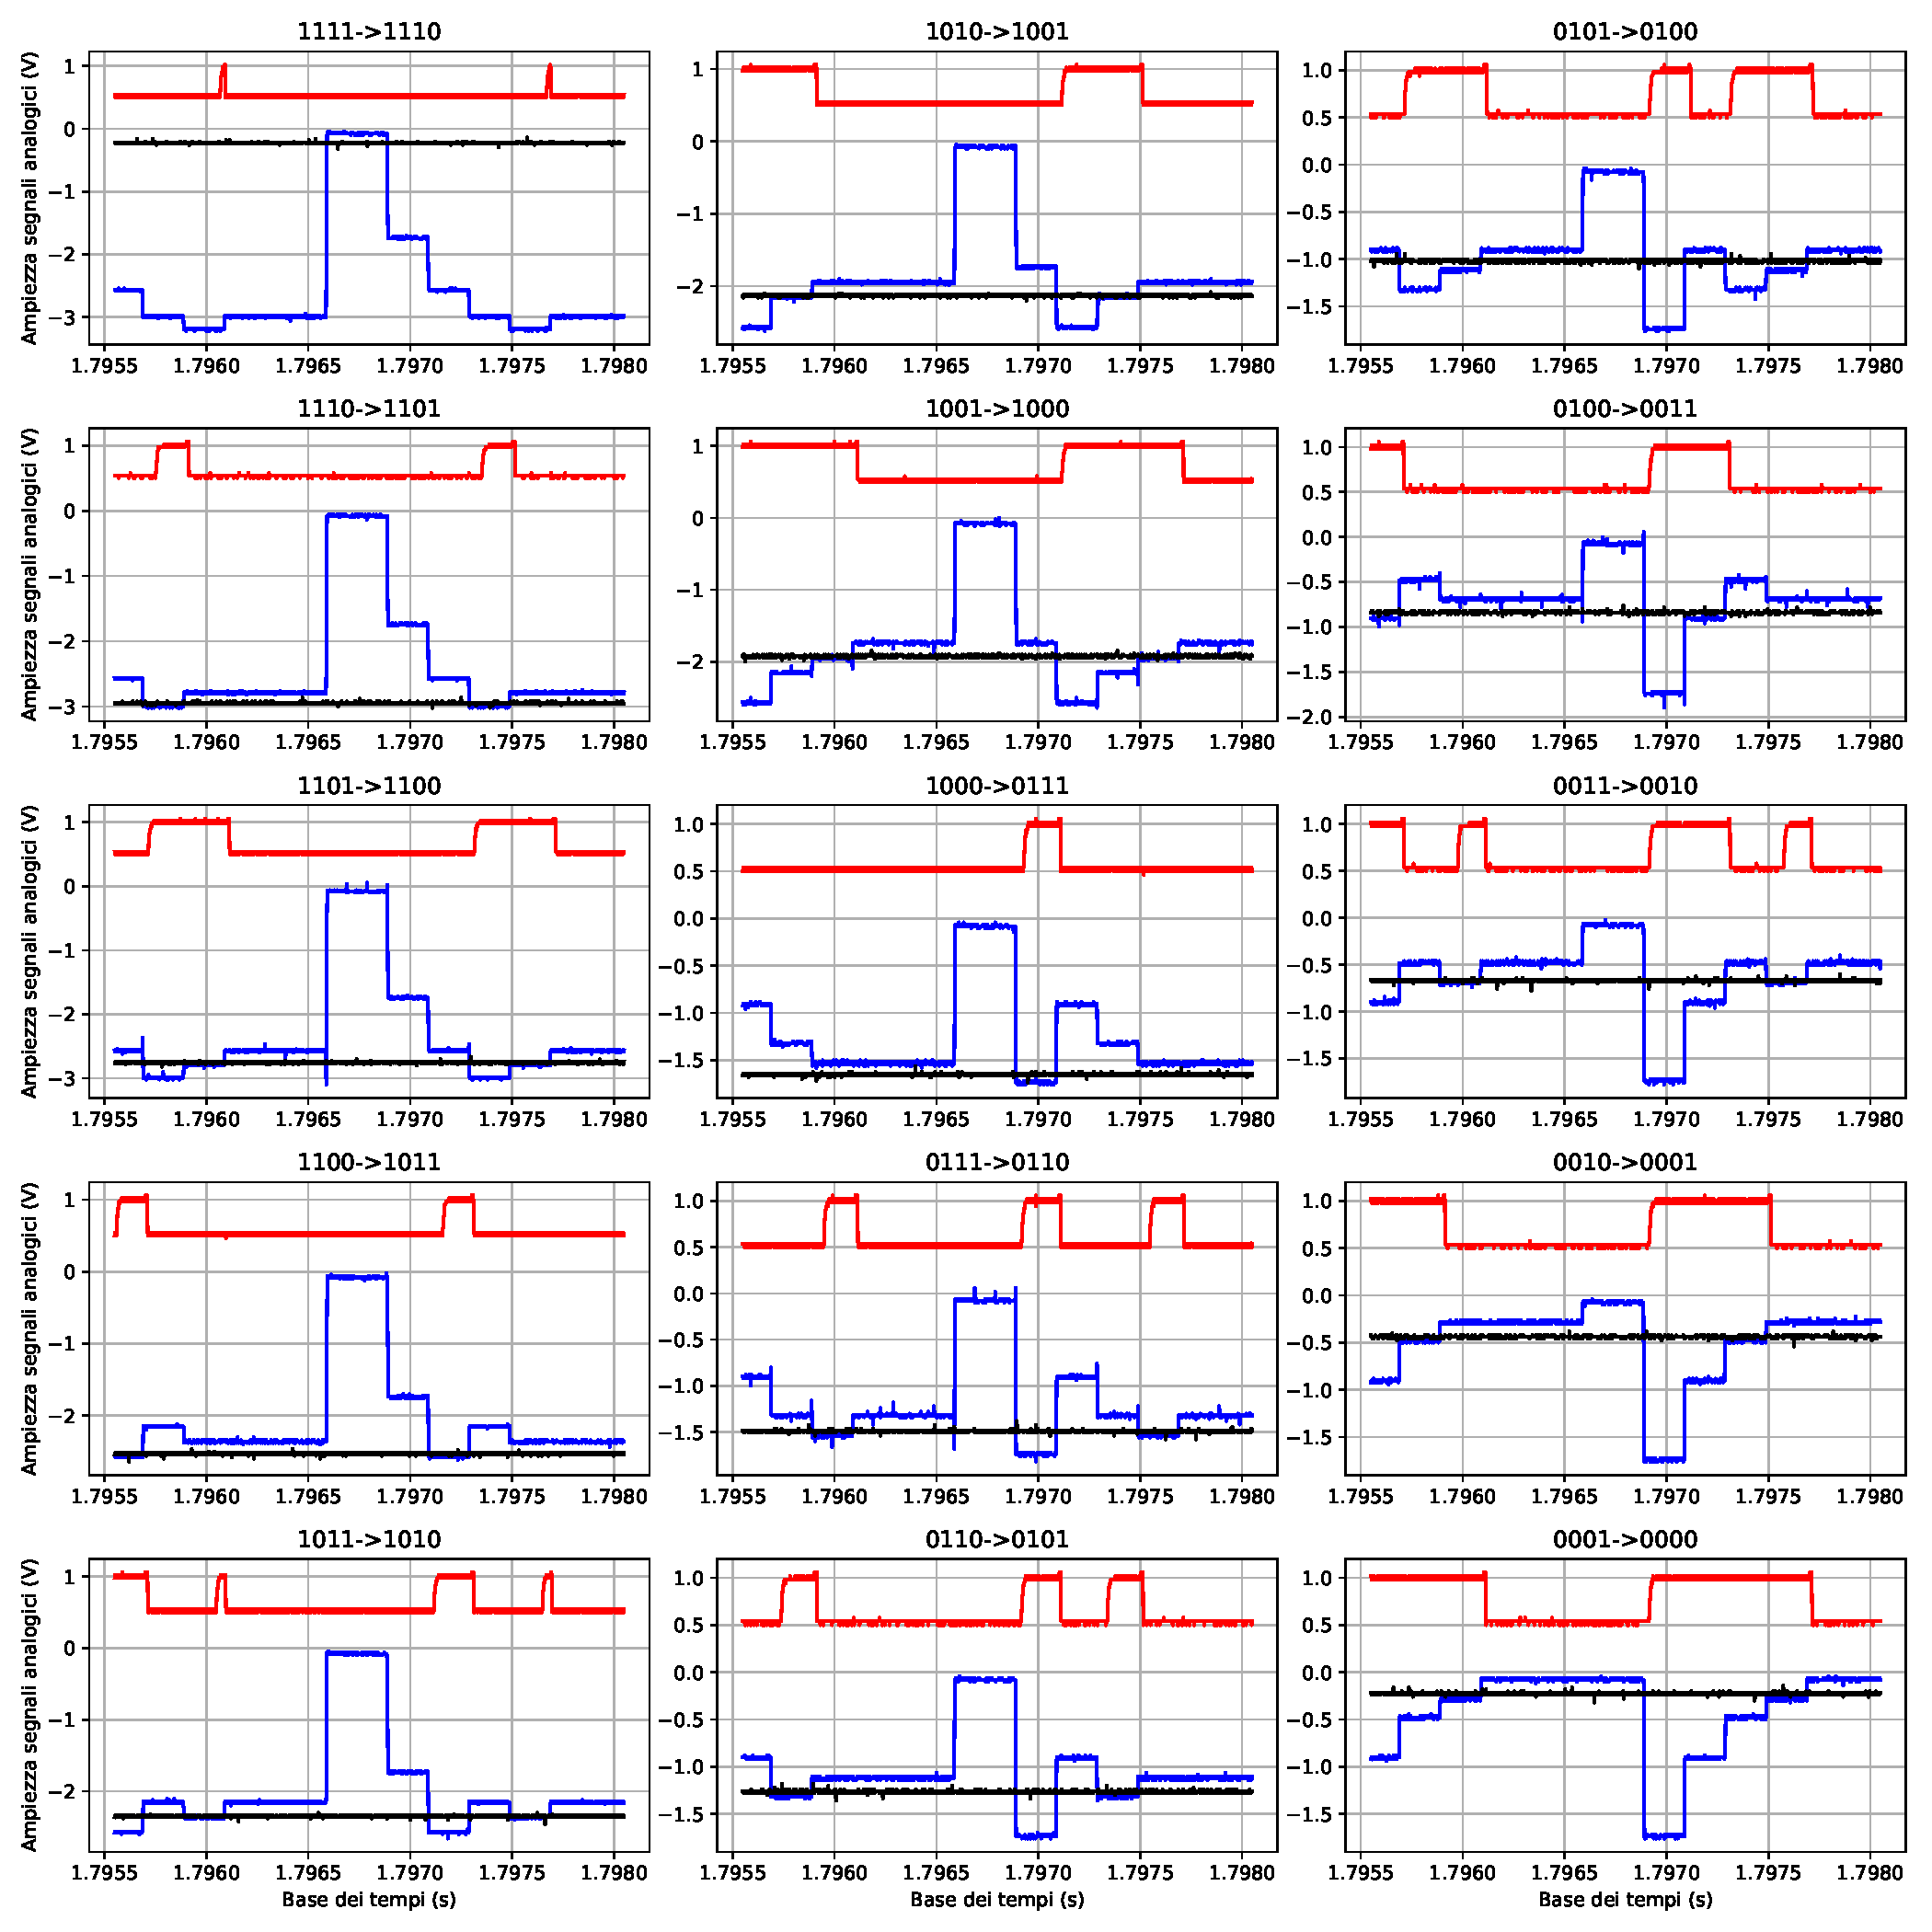
\includegraphics[trim = {30 0 50 0}, width=0.95\textwidth]{analysis/output/calibration.pdf}
\caption{Calibrazione dell'ADC}
\label{fig:waveforms_no_sh_scope}
\end{figure*}

%%%%%%%%%%%%%%%%%%%%%%%%%%%%%%%%%%%%%%%%%%%%%%%%%%%%%%%%%%%%%
\section{Campionamento di tensioni variabili}
Testo

\begin{figure}[H]%[!ht]
\begin{center}
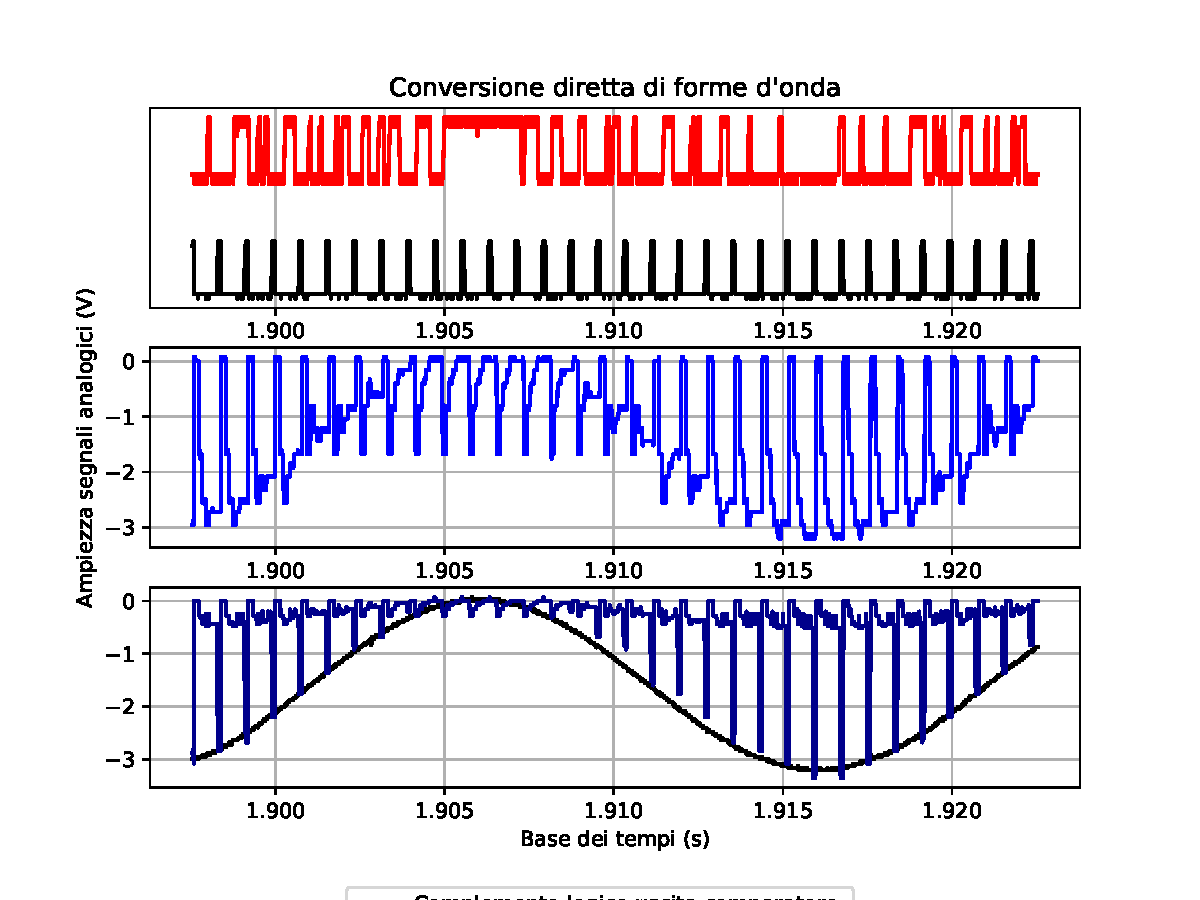
\includegraphics[trim = {0 25 0 0},clip, width=0.50\textwidth]{analysis/output/direct_aq_waveforms.pdf}
\caption{Didascalia}
\label{fig:circuit_DAC}
\end{center}
\end{figure}

\begin{figure}[H]%[!ht]
\begin{center}
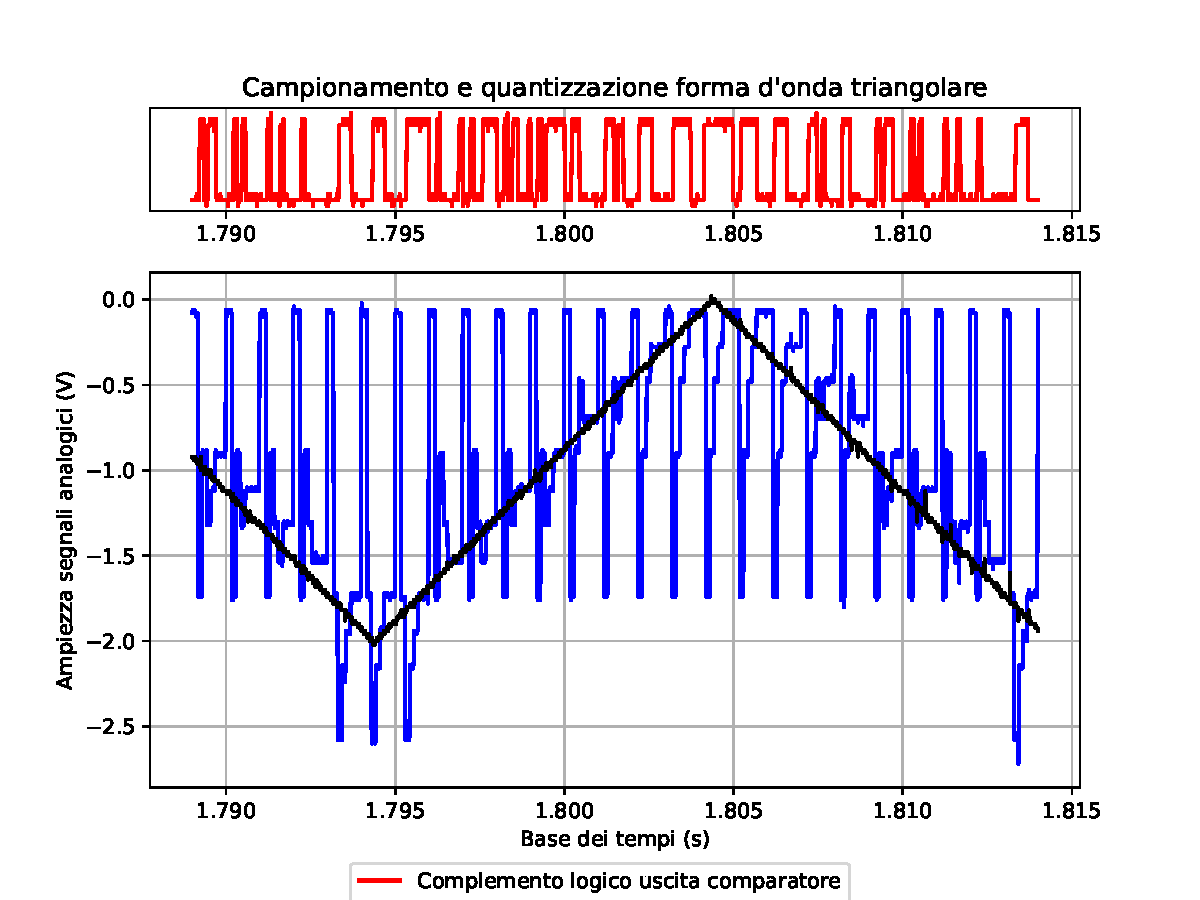
\includegraphics[trim = {0 25 0 0},clip, width=0.50\textwidth]{analysis/output/triangle_wave_aq.pdf}
\caption{Didascalia}
\label{fig:circuit_DAC}
\end{center}
\end{figure}

\begin{figure}[H]%[!ht]
\begin{center}
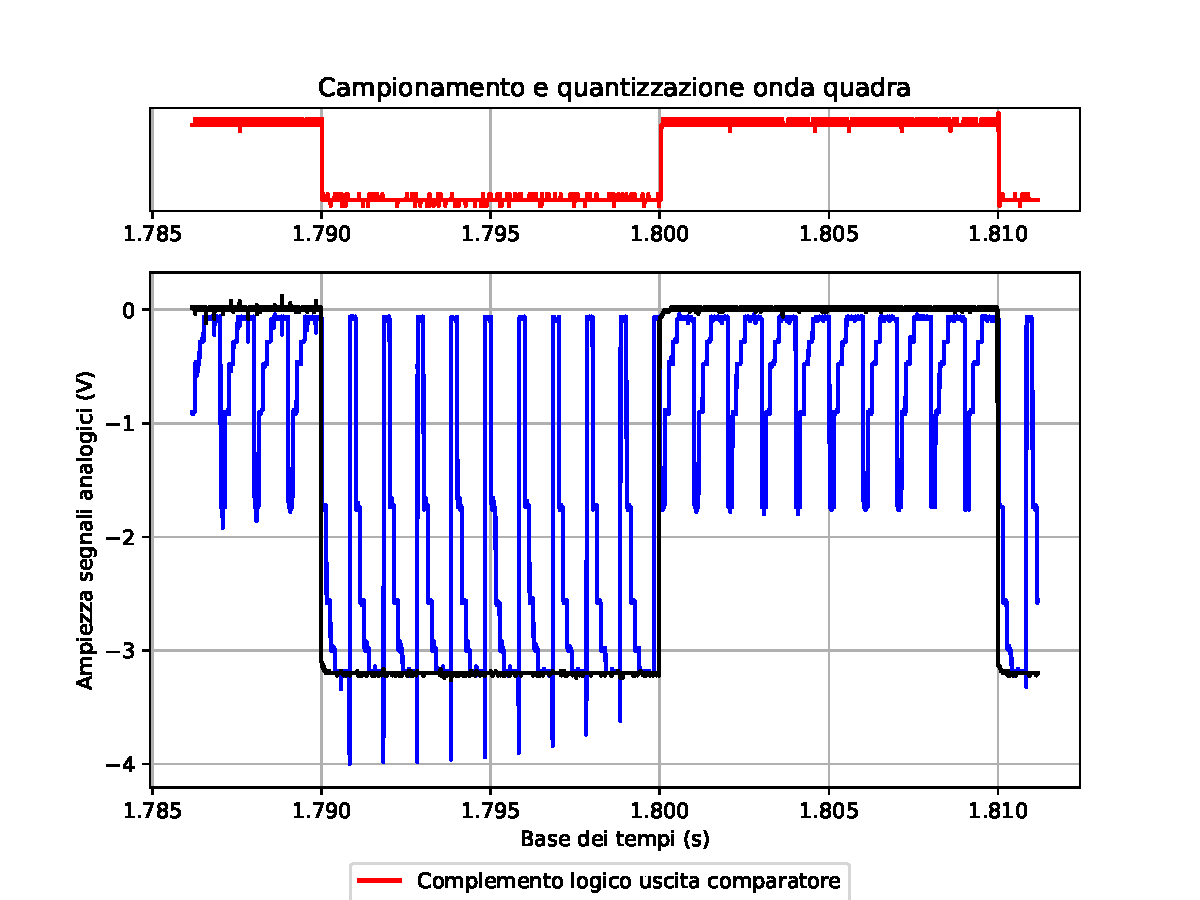
\includegraphics[trim = {0 25 0 0},clip, width=0.50\textwidth]{analysis/output/square_wave_aq.pdf}
\caption{Didascalia}
\label{fig:circuit_DAC}
\end{center}
\end{figure}

\begin{figure*}[t]%[t]
\centering
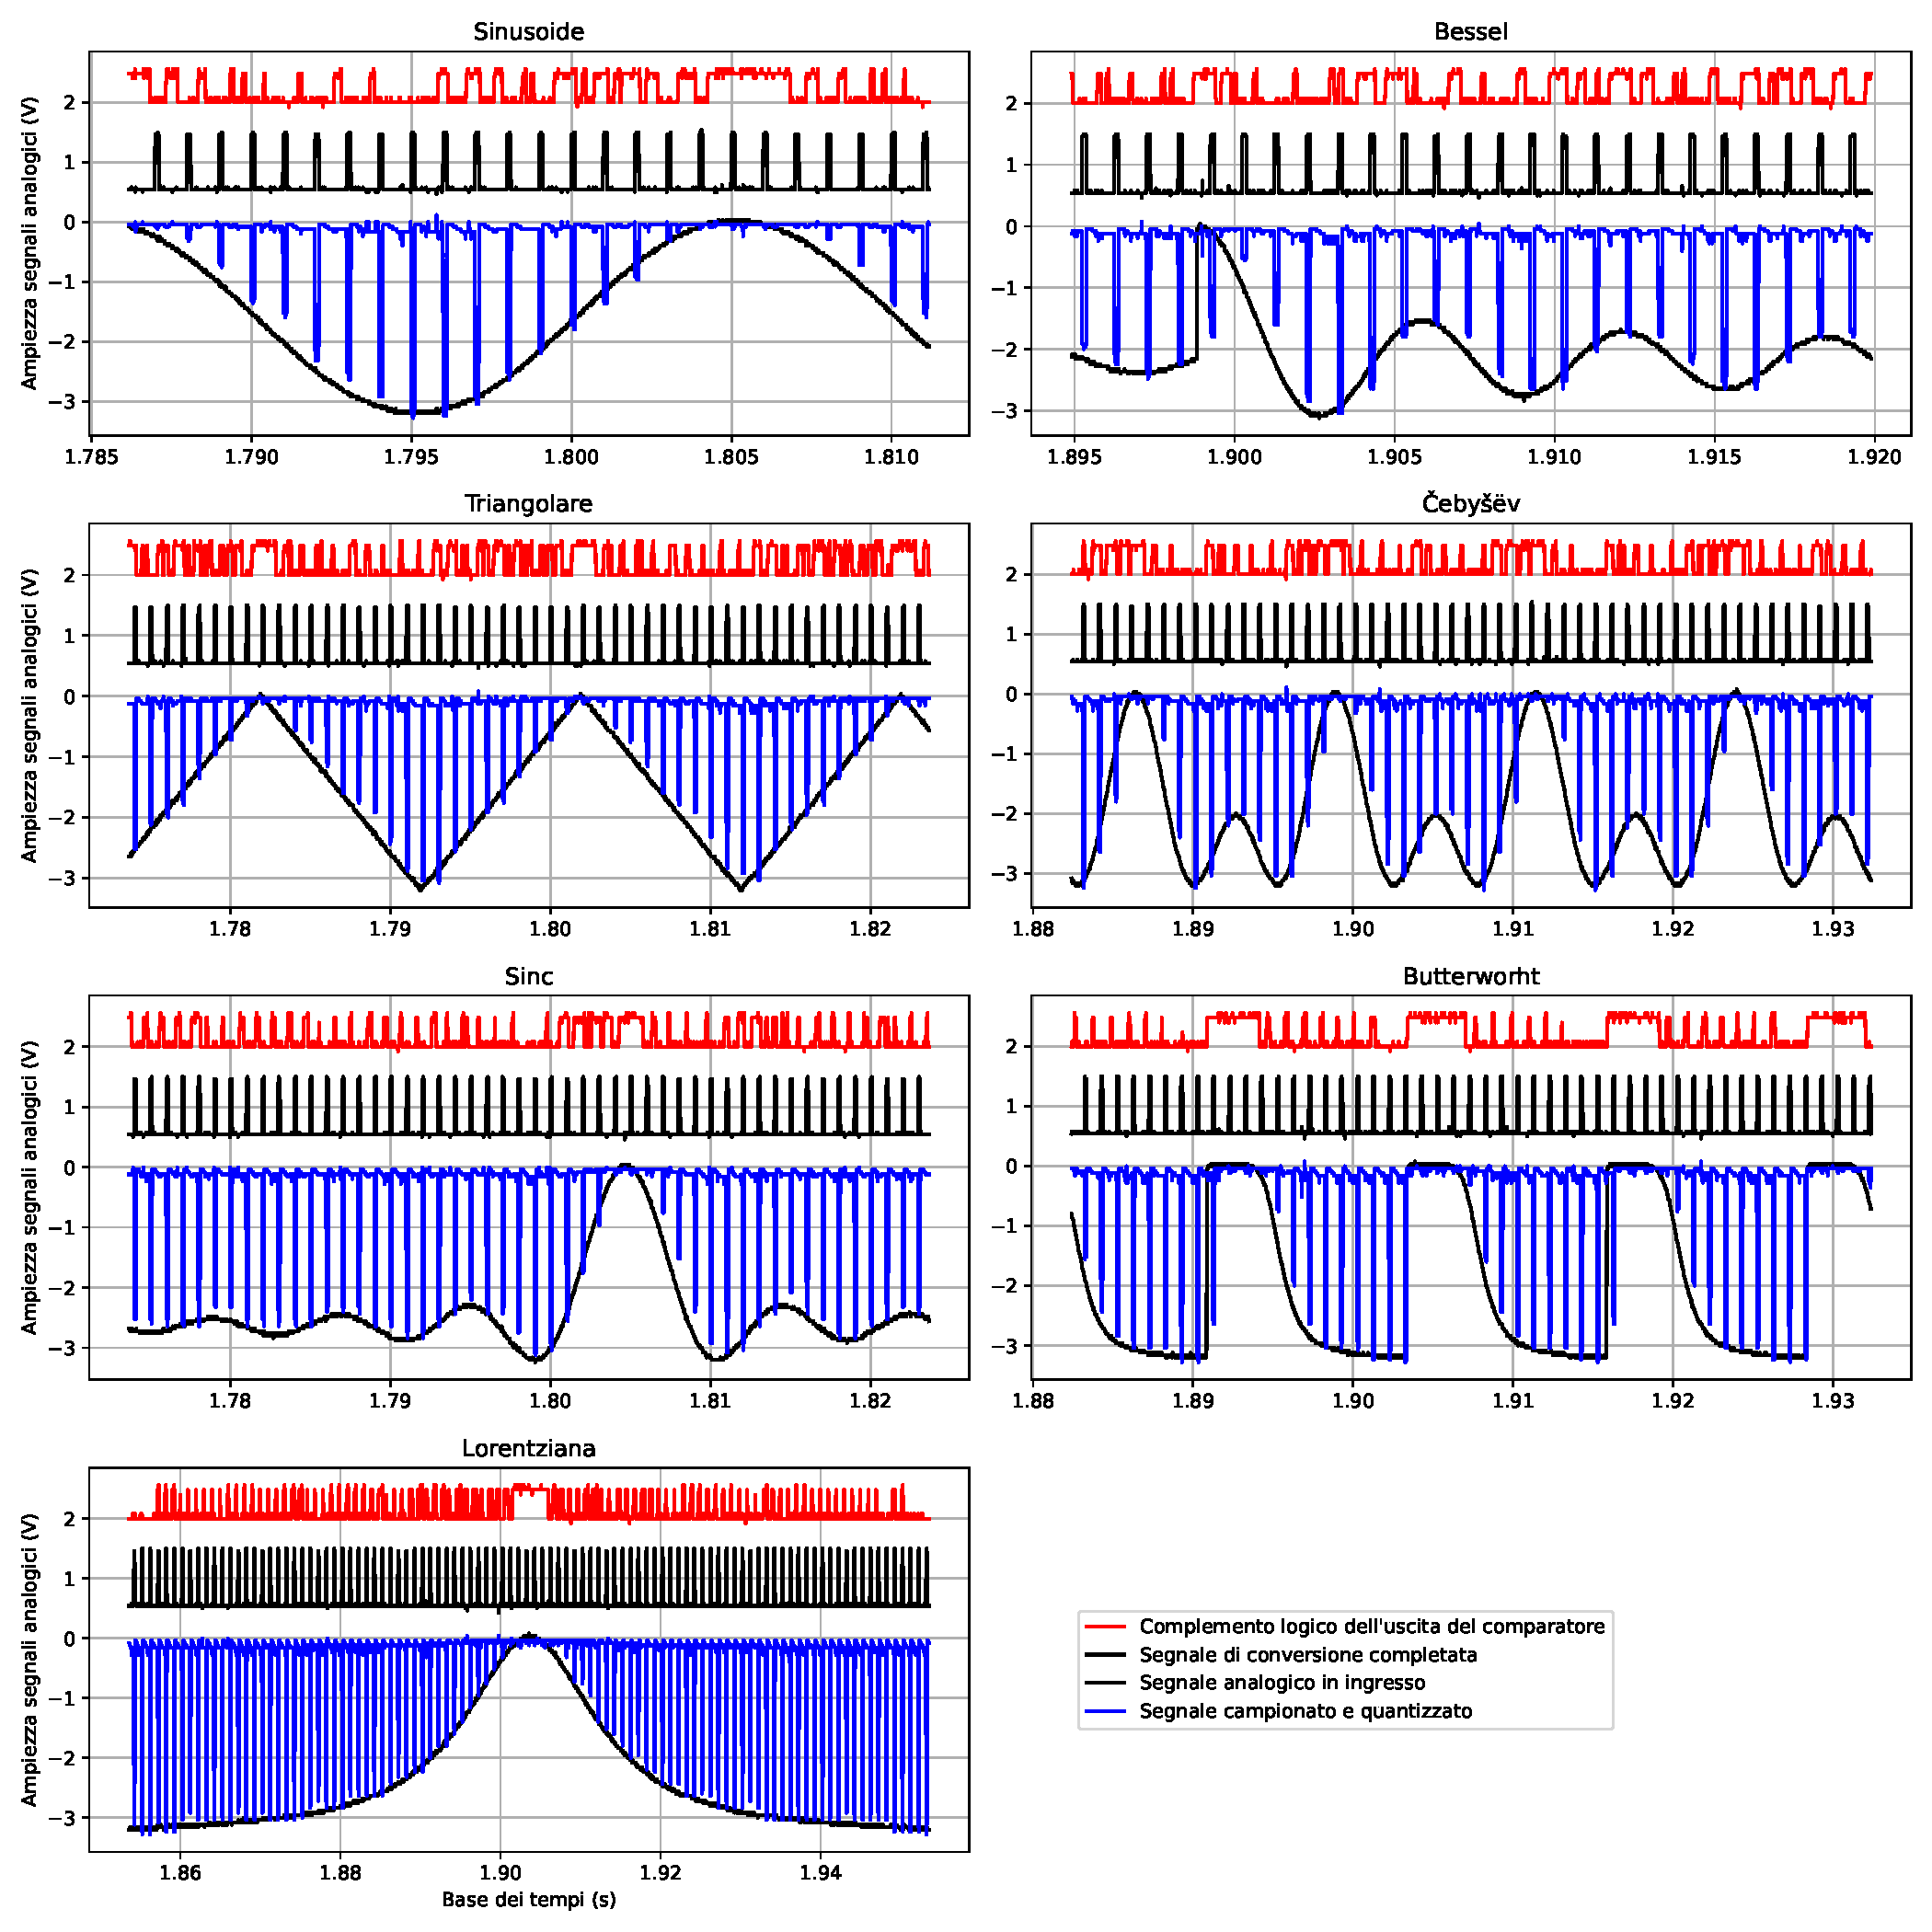
\includegraphics[trim = {30 0 50 0}, width=0.95\textwidth]{analysis/output/waveforms.pdf}
\caption{Schema elettrico completo del convertitore ADC SAR 4 bit}
\label{fig:waveforms_no_sh_scope}
\end{figure*}



\subsection{Circuito \textit{sample-hold}}
Finora è stato possibile eseguire il campionamento di segnali variabili nel tempo solamente sotto l'ipotesi di variazione lenta rispetto al tempo di campionamento dell'ADC. Questa ipotesi è necessaria perché il processo di approssimazioni successive dà risultati coerenti solo se durante le operazioni di confronto con l'uscita del DAC il segnale analogico in ingresso rimane pressoché costante. Per poter lavorare con segnali in ingresso più veloci, fino al limite teorico imposto dal teorema del campionamento di Nyquist-Shannon che discuteremo in seguito, si rende quindi necessaria l'introduzione di un circuito \textit{sample \& hold} che nel nostro apparato è stato realizzato con un integrato LF398. Tale componente è controllato dall'uscita $Q_F$ del registro di scorrimento: quando questo segnale digitale è alto la tensione in uscita dall'integrato insegue l'ingresso (campionamento), mentre quanto si abbassa, grazie al condensatore $C_h$, l'integrato mantiene l'uscita fissa al valore che aveva al fronte di discesa di $Q_F$. Questo fa sì che quando saranno alte le uscite del registro da $Q_A$ a $Q_E$ (operazioni di confronto) LF398 sia in modalità \textit{hold}.


\begin{figure}[H]%[!ht]
\begin{center}
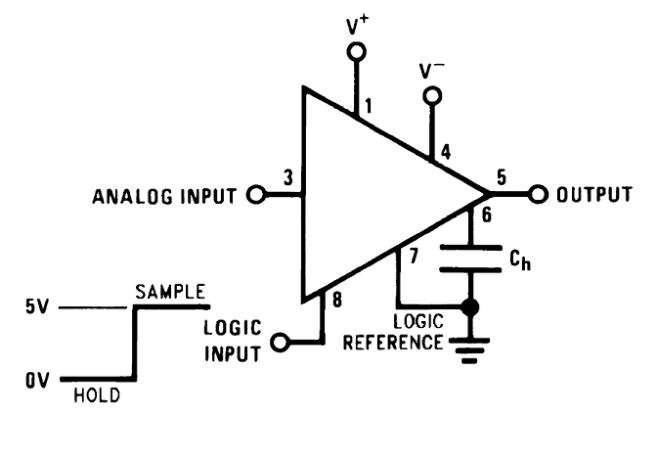
\includegraphics[width=0.35\textwidth]{sch-simulations/digital/output/lf398.png}
\caption{Schema di collegamento dell'integrato LF398 utilizzato in laboratorio per realizzare il circuito di \textit{sample and hold}, proveniente dal datasheet Texas Instruments del componente. Il valore del condensatore è $C_h$ = (10.5 $\pm$ 0.4) nF}
\label{fig:circuit_sample_and_hold}
\end{center}
\end{figure}

%%%%%%%%%%%%%%%%%%%%%%%%%%%%%%%%%%%%%%%%%%%%%%%%%%%%%%%%%%%%%
\section{Registrazione della conversione mediante scheda a microcontrollore}
Testo

\subsection{Verifica del teorema del campionamento di Nyquist-Shannon con sample-hold e oscilloscopio}
Testo

\clearpage
\clearpage
\begin{figure}[H]%[!ht]
\begin{center}
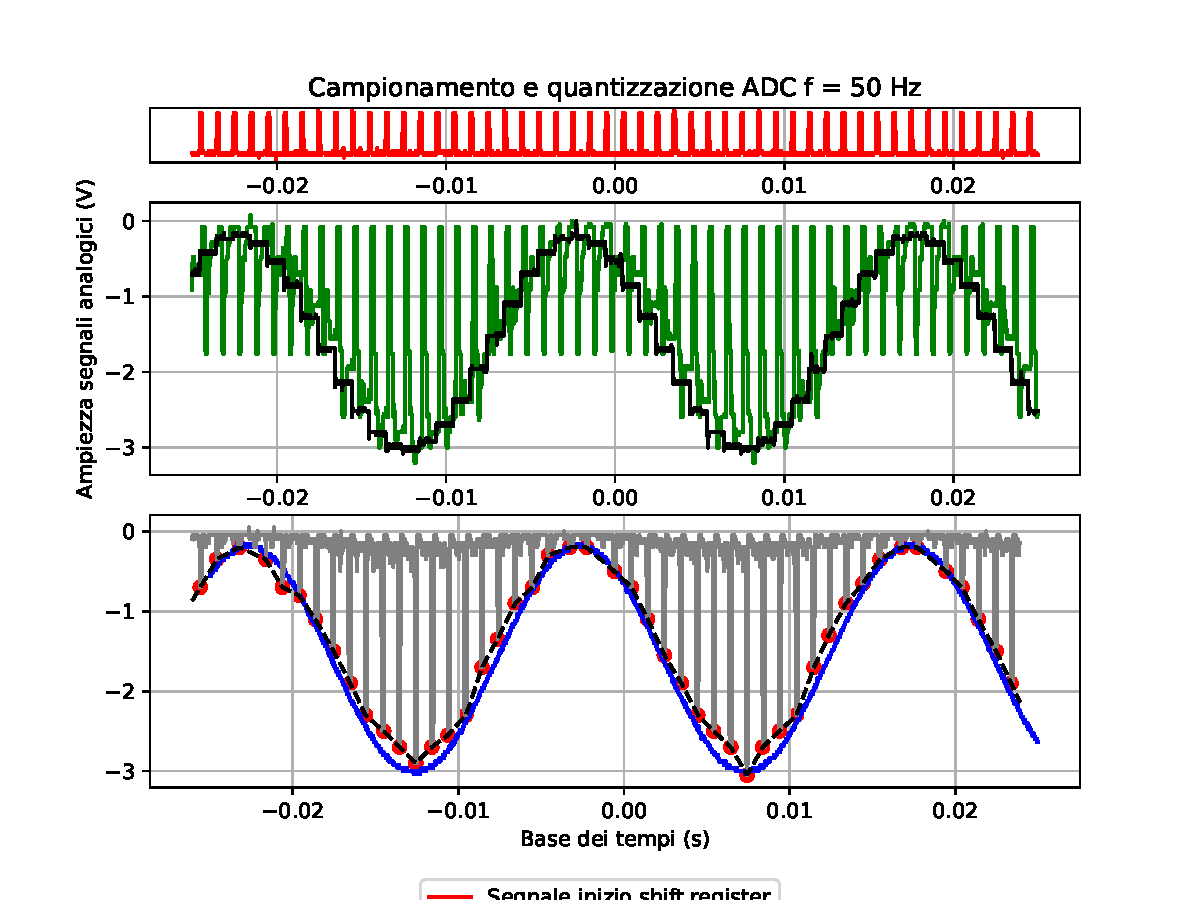
\includegraphics[trim={0 25 0 0}, clip, width=0.50\textwidth]{analysis/output/campionamento_50Hz.pdf}

\caption{Campionamento di forma d'onda sinusoidale f = 50 Hz. In rosso il segnale logico di controllo del sample-hold, in nero il segnale in uscita dal sample-hold, in verde il segnale in uscita dal DAC, il blu il segnale analogico in ingresso e in grigio il segnale ricostruito dall'ADC.}
\label{fig:sampSH1}
\end{center}
\end{figure}
\vspace{-10mm}
%
\begin{figure}[H]%[!ht]
\begin{center}
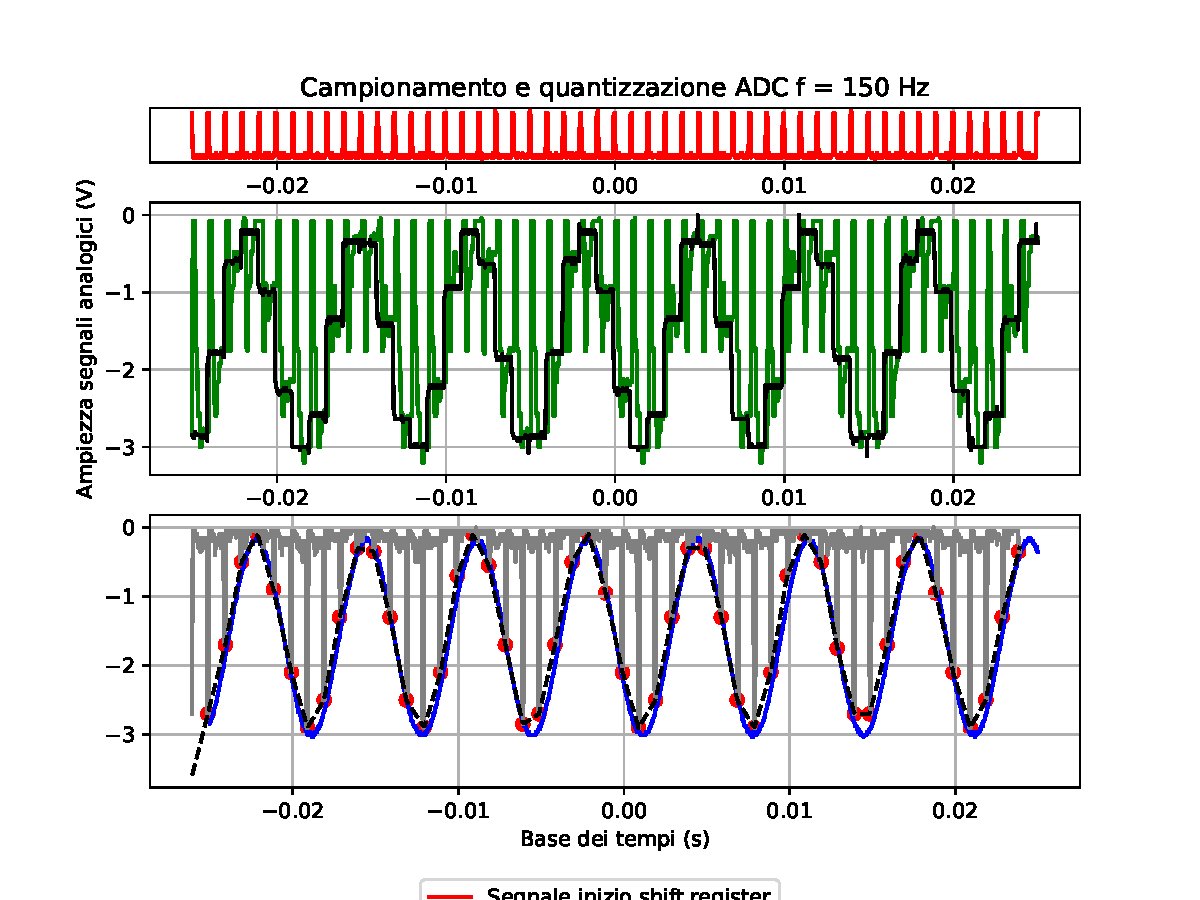
\includegraphics[trim={0 25 0 0}, clip,width=0.50\textwidth]{analysis/output/campionamento_150Hz.pdf}
\caption{Campionamento di forma d'onda sinusoidale f = 150 Hz, colori come nella figura precedente.}
\label{fig:sampSH2}
\end{center}
\end{figure}
\vspace{-10mm}
%
\begin{figure}[H]%[!ht]
\begin{center}
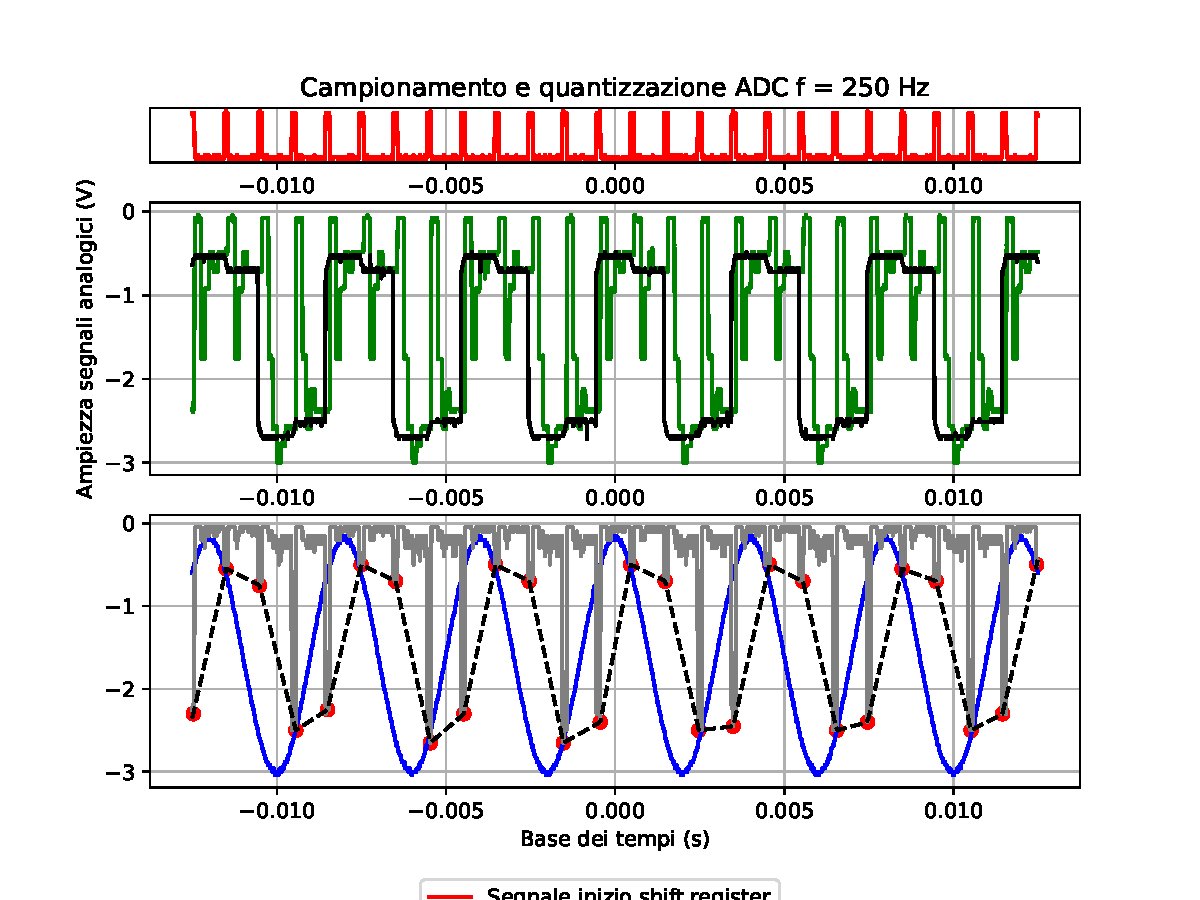
\includegraphics[trim={0 25 0 0}, clip,width=0.50\textwidth]{analysis/output/campionamento_250Hz.pdf}
\caption{Campionamento di forma d'onda sinusoidale f = 250 Hz, colori come nella figura precedente.}
\label{fig:sampSH3}
\end{center}
\end{figure}
\vspace{-10mm}
%
\begin{figure}[H]%[!ht]
\begin{center}
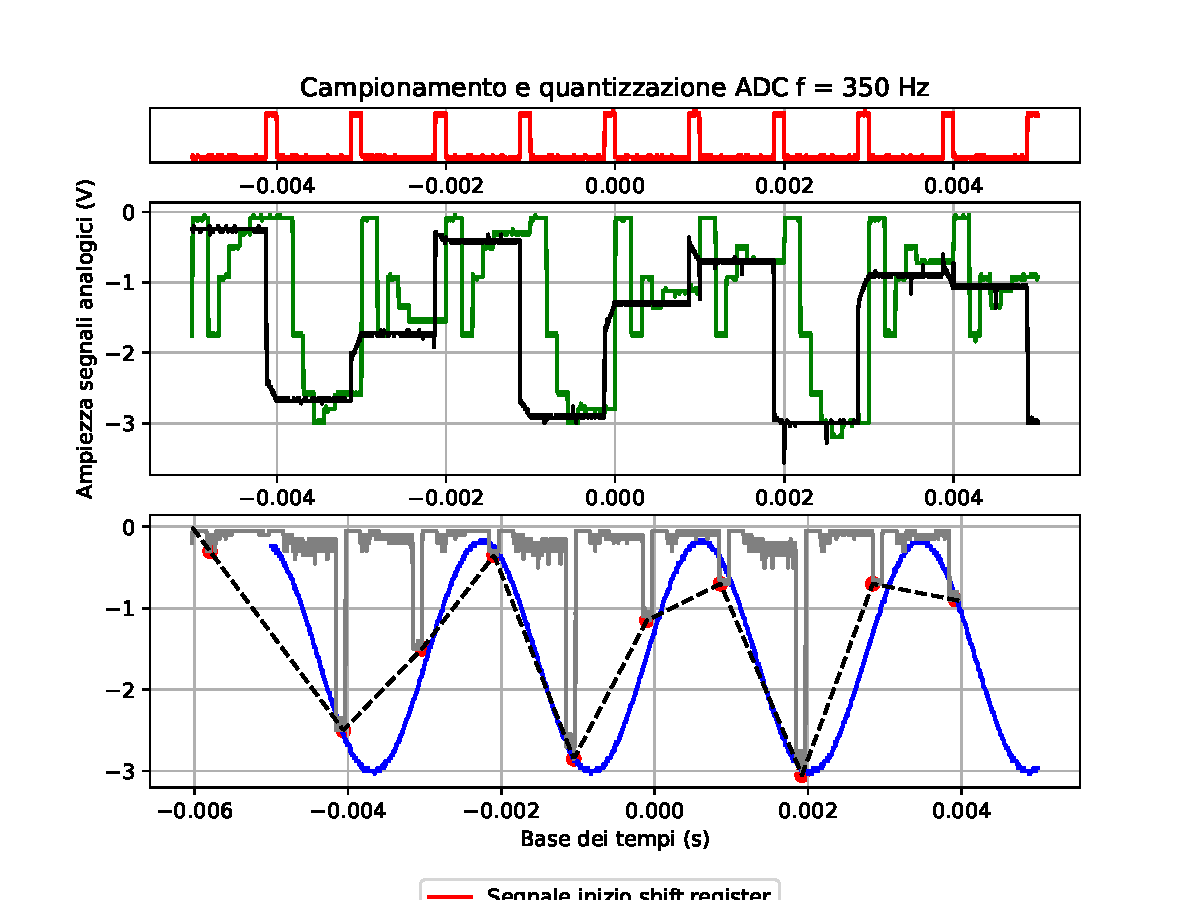
\includegraphics[trim={0 40 0 0}, clip,width=0.50\textwidth]{analysis/output/campionamento_350Hz.pdf}
\caption{Campionamento di forma d'onda sinusoidale f = 350 Hz, colori come nella figura precedente.}
\label{fig:sampSH4}
\end{center}
\end{figure}
\vspace{-10mm}
%
\begin{figure}[H]%[!ht]
\begin{center}
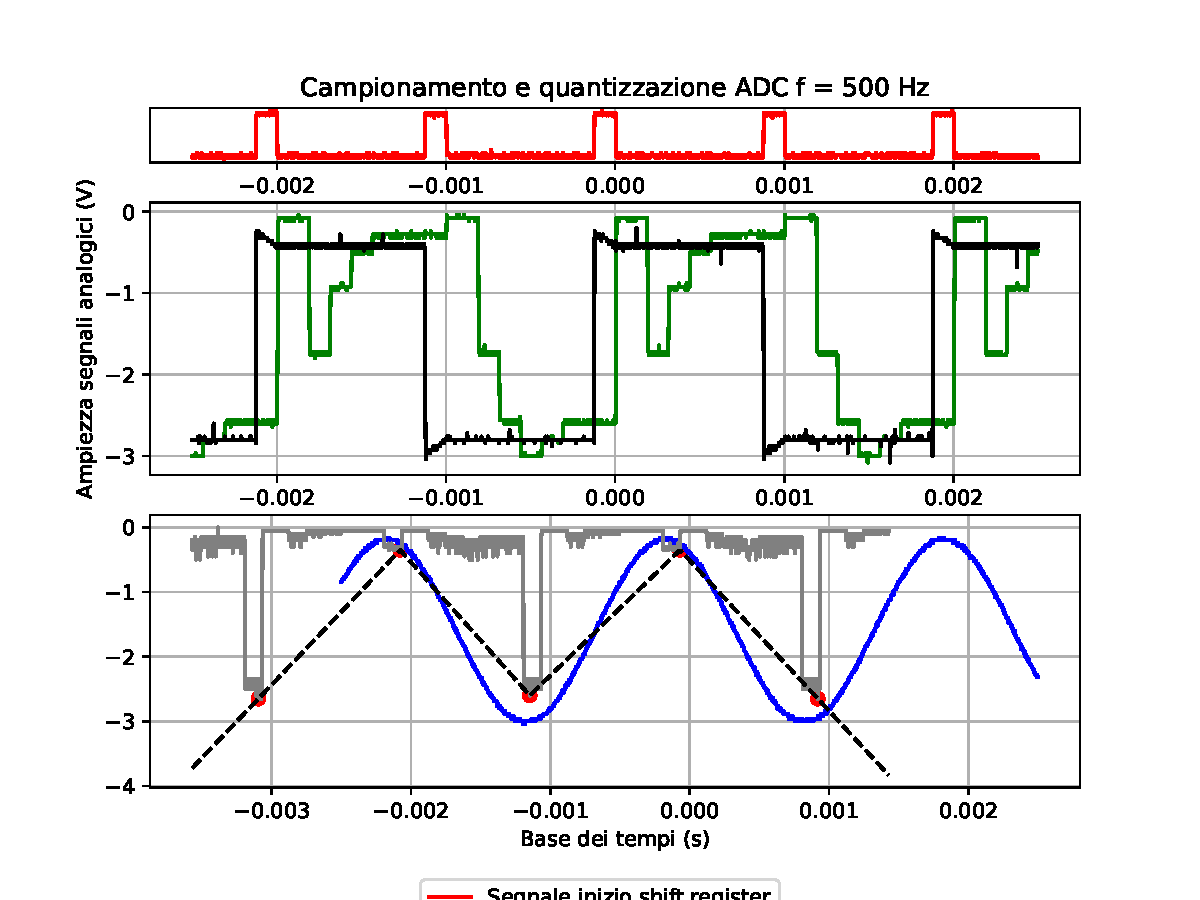
\includegraphics[trim={0 40 0 0}, clip,width=0.50\textwidth]{analysis/output/campionamento_500Hz.pdf}
\caption{Campionamento di forma d'onda sinusoidale f = 500 Hz, colori come nella figura precedente.}
\label{fig:sampSH5}
\end{center}
\end{figure}
\vspace{-10mm}
%
\begin{figure}[H]%[!ht]
\begin{center}
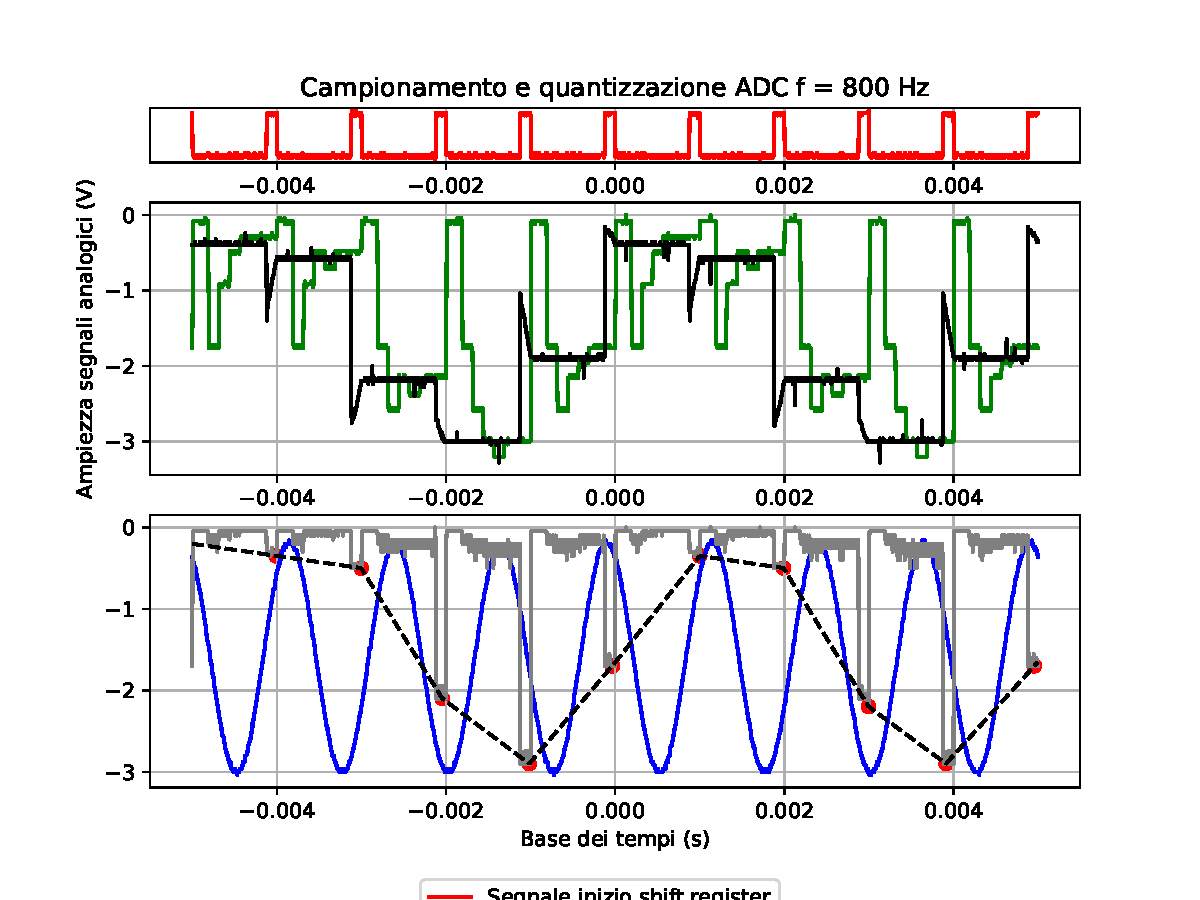
\includegraphics[trim={0 40 0 0}, clip,width=0.50\textwidth]{analysis/output/campionamento_800Hz.pdf}
\caption{Campionamento di forma d'onda sinusoidale f = 800 Hz, colori come nella figura precedente.}
\label{fig:sampSH6}
\end{center}
\end{figure}

\subsection{Verifica del teorema del campionamento di Nyquist-Shannon con sample-hold e acquisizione con microcontrollore}

%% Ridurre numero di immagini, cambiare dimensione

\clearpage 
\begin{figure*}[t]%[t]
\centering
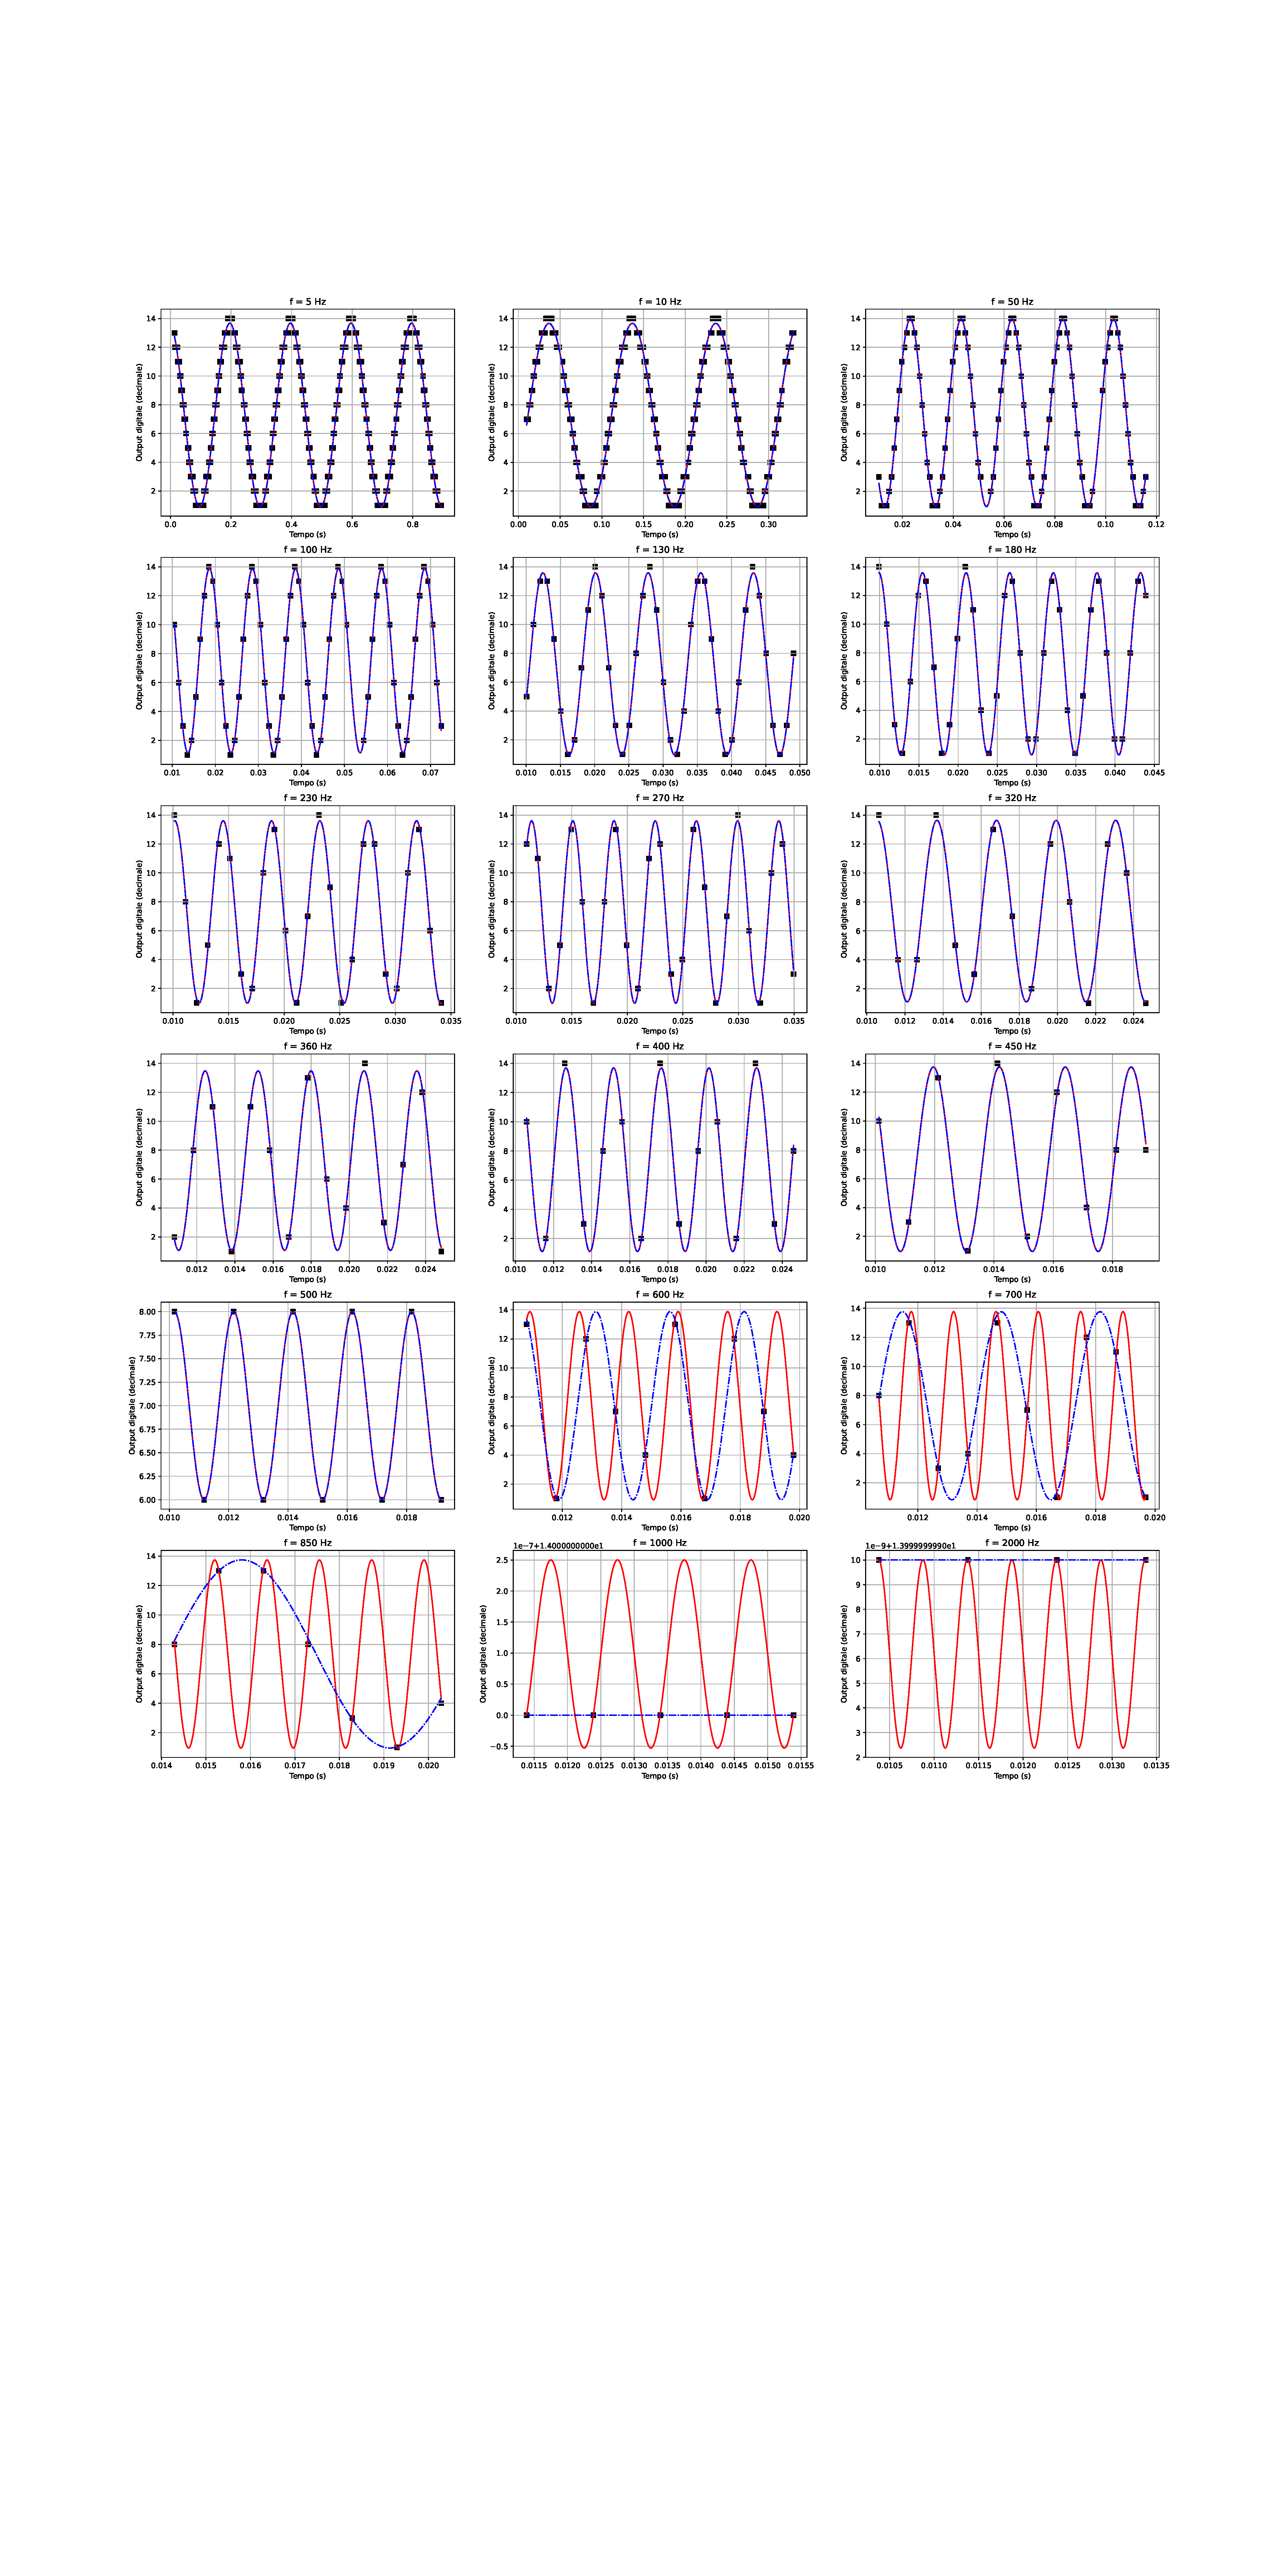
\includegraphics[trim = {150 0 0 400}, width=1.1\textwidth]{analysis/output/cumulative_nyquist_mcu.pdf}
\caption{campionamento di segnale sinusoidale con frequenze da 5 a 2000 Hz}
\label{fig:nyquist_mcu_cumulative}
\end{figure*}



\subsection{Valutazione della linearità con metodo della \textit{code density}}

Istogrammi delle frequenze di occupazione dei codici

\begin{figure}[H]%[!ht]
\begin{center}

%1
\caption{$\sigma = 0.033$}
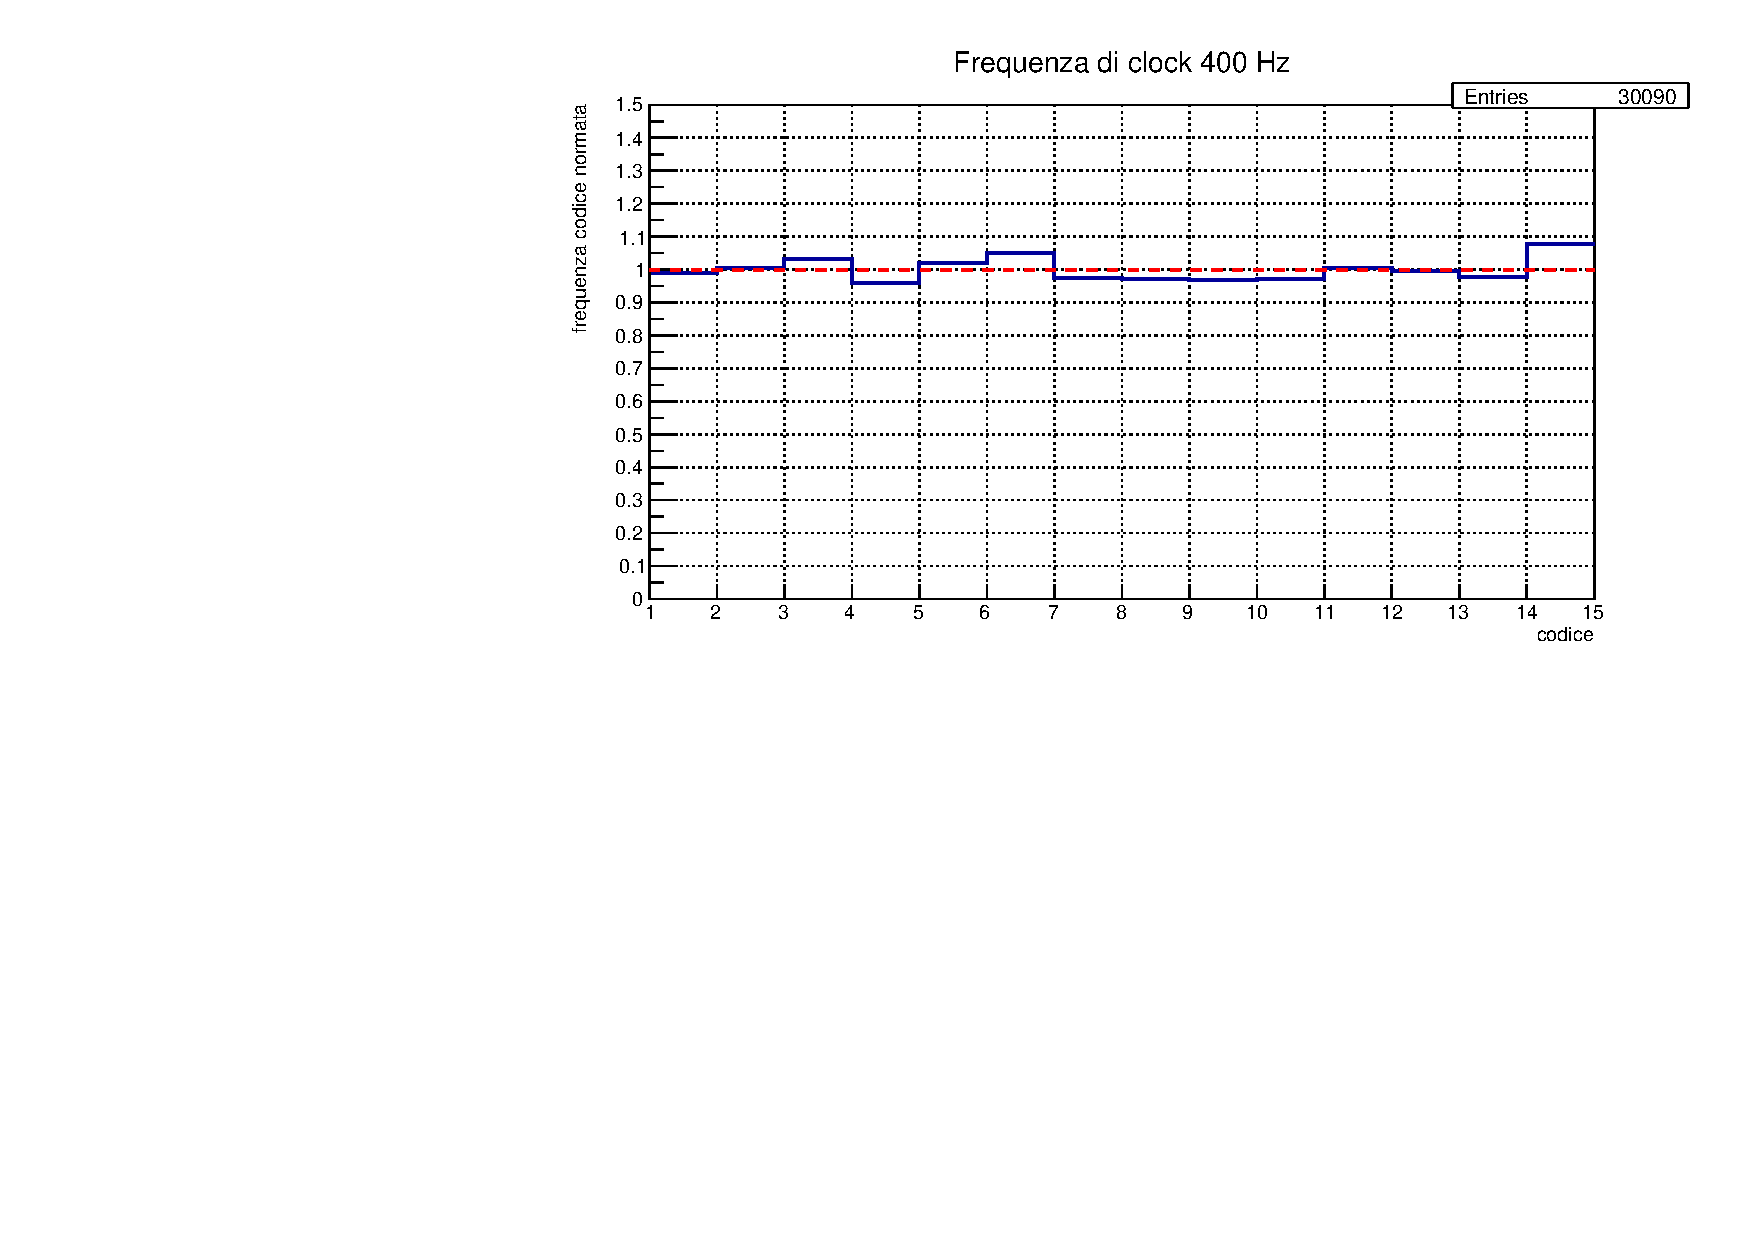
\includegraphics[width=0.48\textwidth]{analysis/output/dnl_1_400hz_bars.pdf}
\label{fig:graph_dnl_400_hz}
%2
\caption{$\sigma = 0.031$}
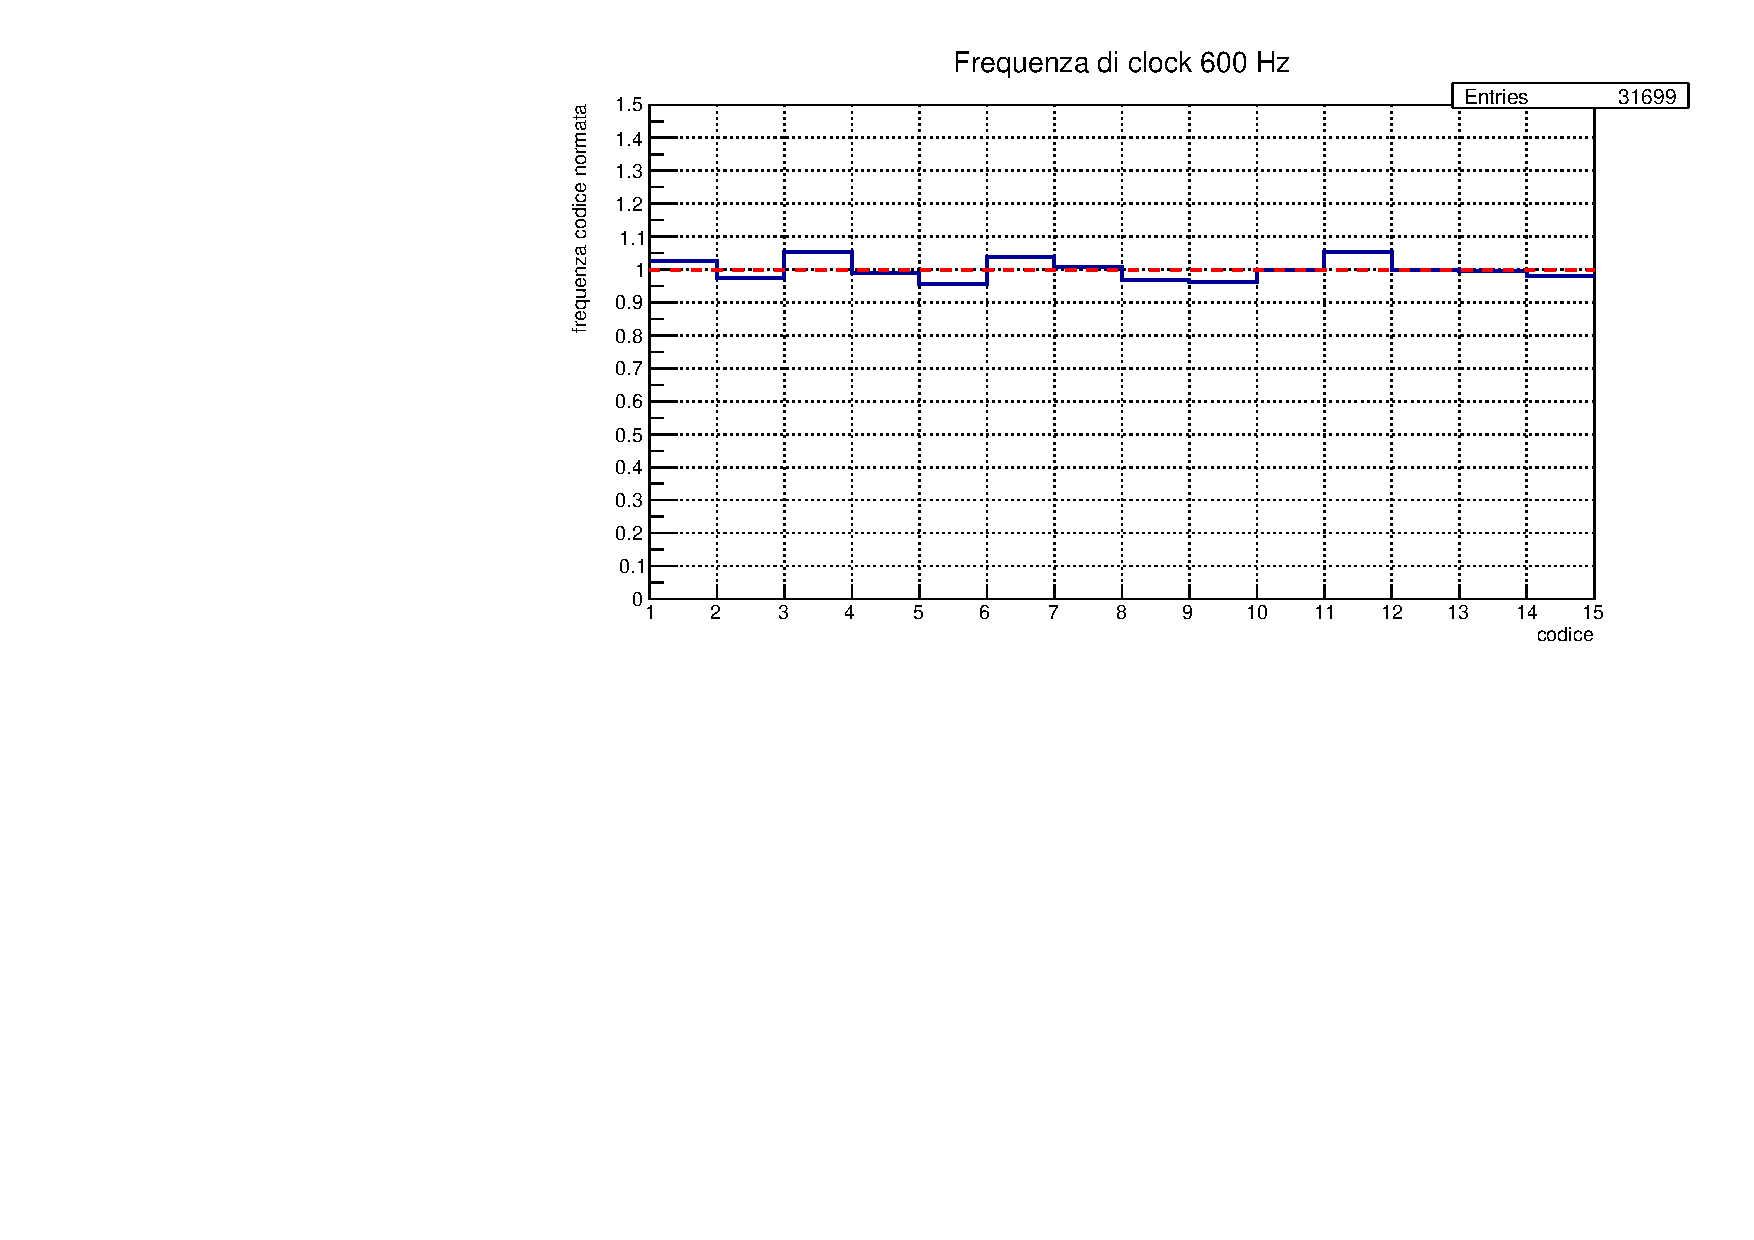
\includegraphics[width=0.48\textwidth]{analysis/output/dnl_2_600hz_bars.pdf}
\label{fig:graph_dnl_600_hz}
%3
\caption{$\sigma = 0.028$}
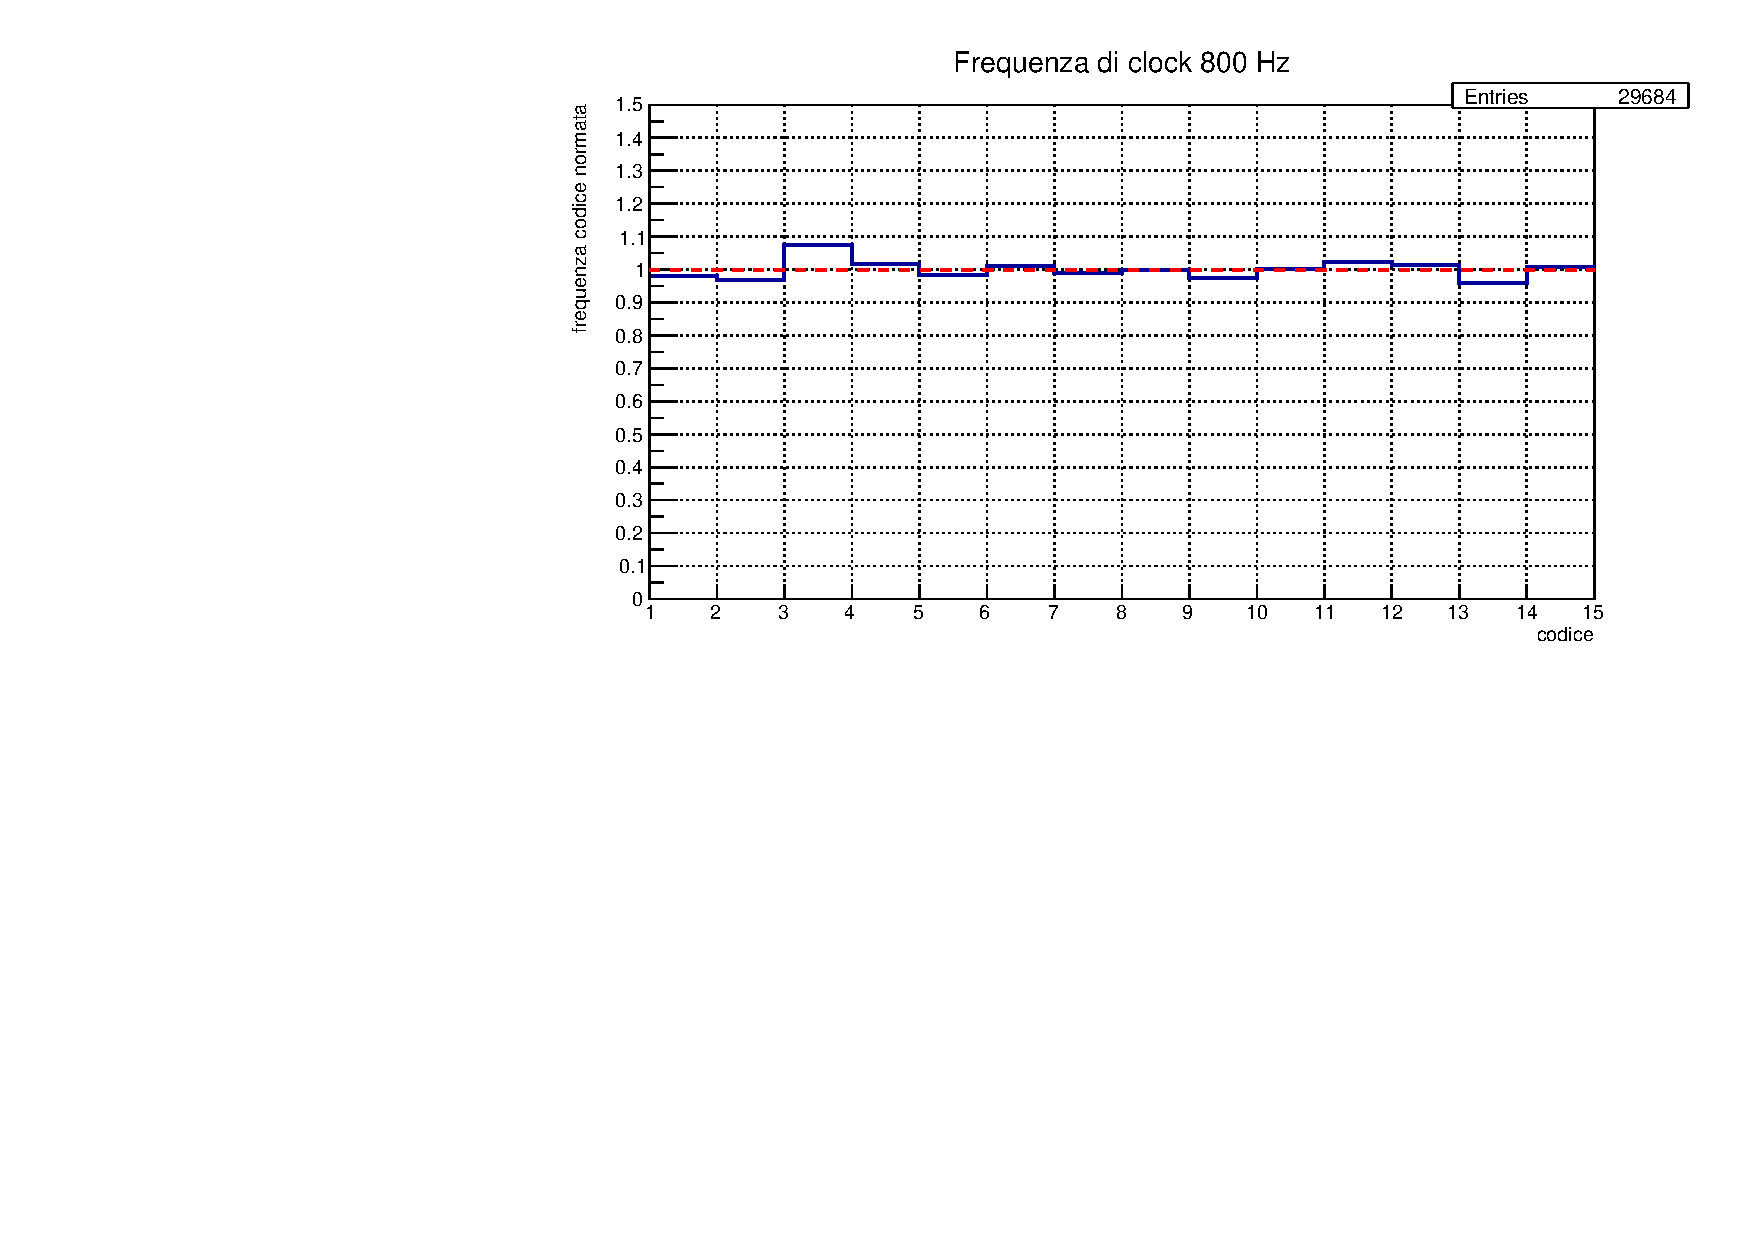
\includegraphics[width=0.48\textwidth]{analysis/output/dnl_3_800hz_bars.pdf}
\label{fig:graph_dnl_800_hz}
%4
\caption{$\sigma = 0.030$}
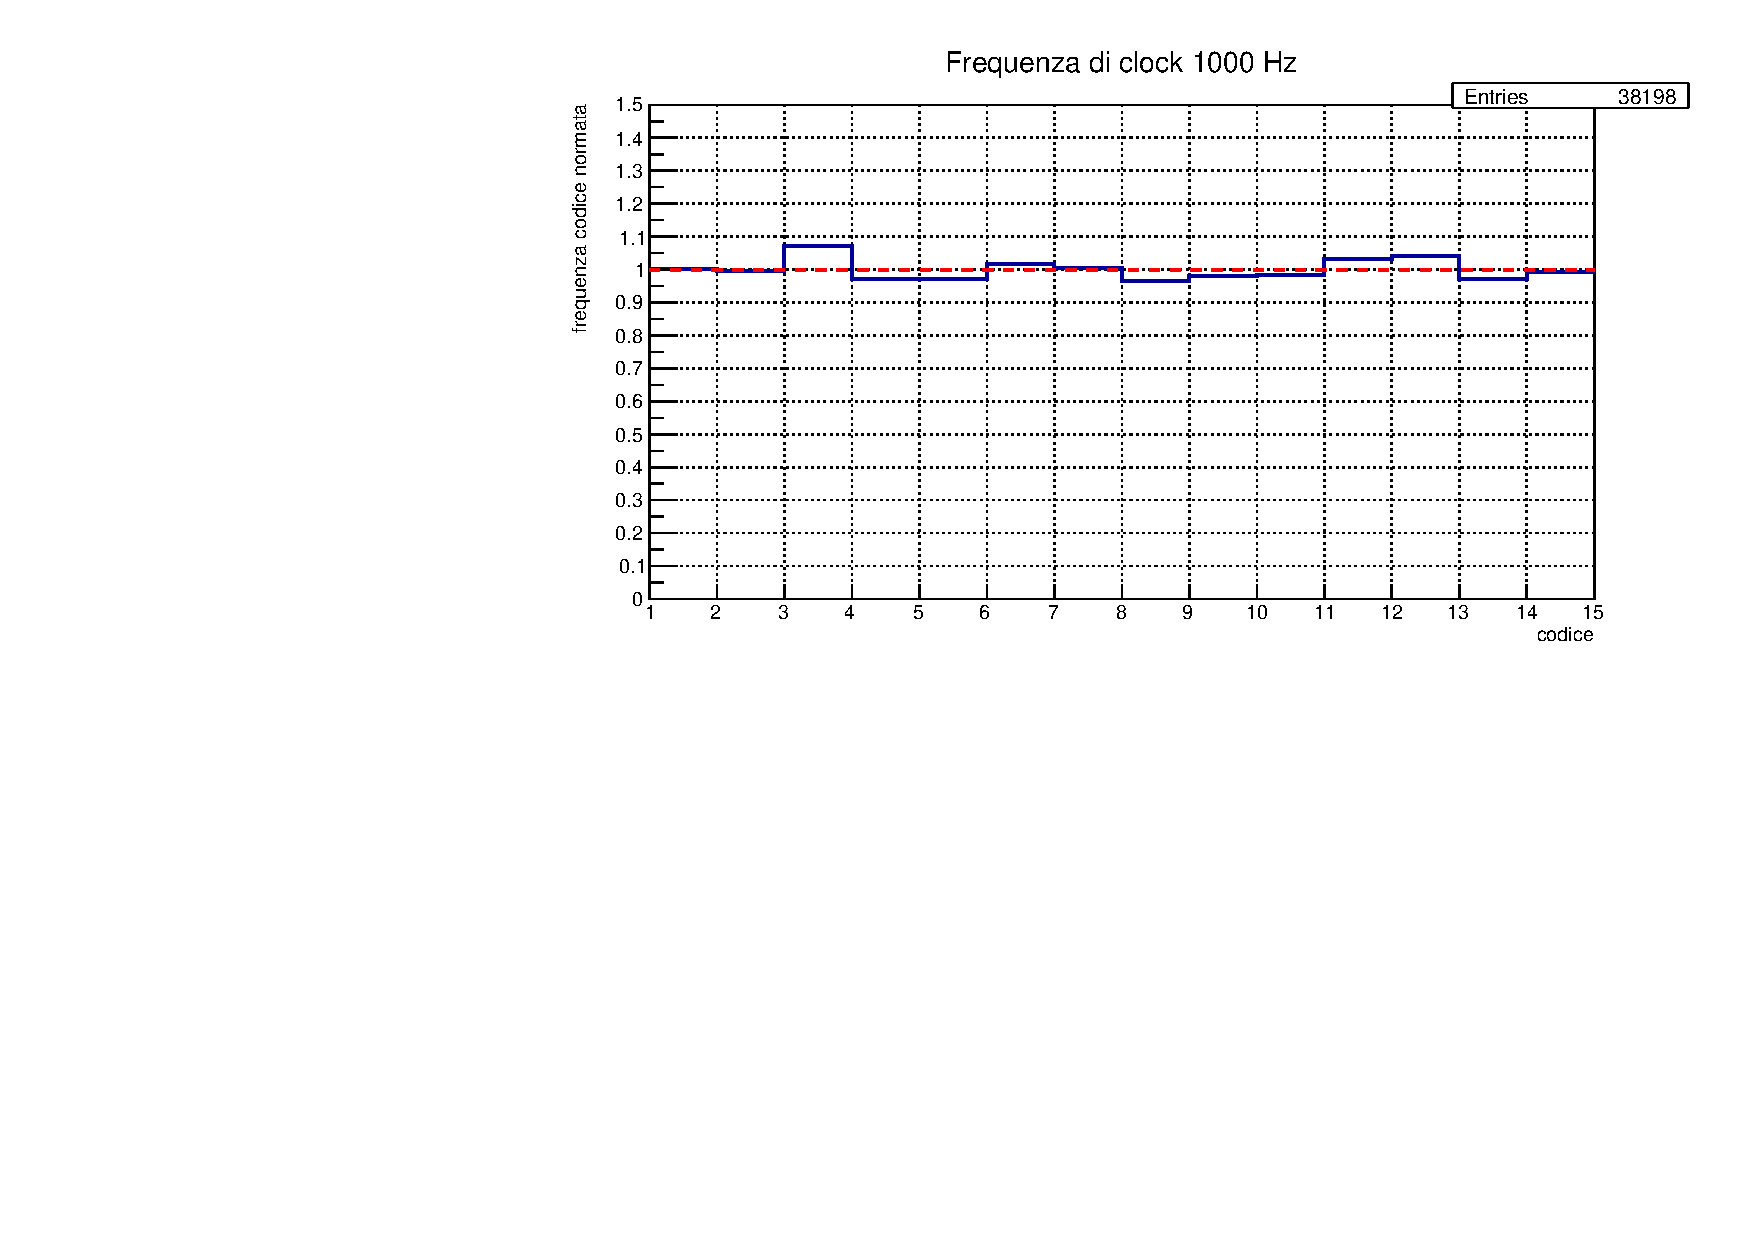
\includegraphics[width=0.48\textwidth]{analysis/output/dnl_4_1000hz_bars.pdf}
\label{fig:graph_dnl_1000_hz}
\end{center}
\end{figure}

\begin{figure}[H]
\begin{center}
%5
\caption{$\sigma = 0.043$}
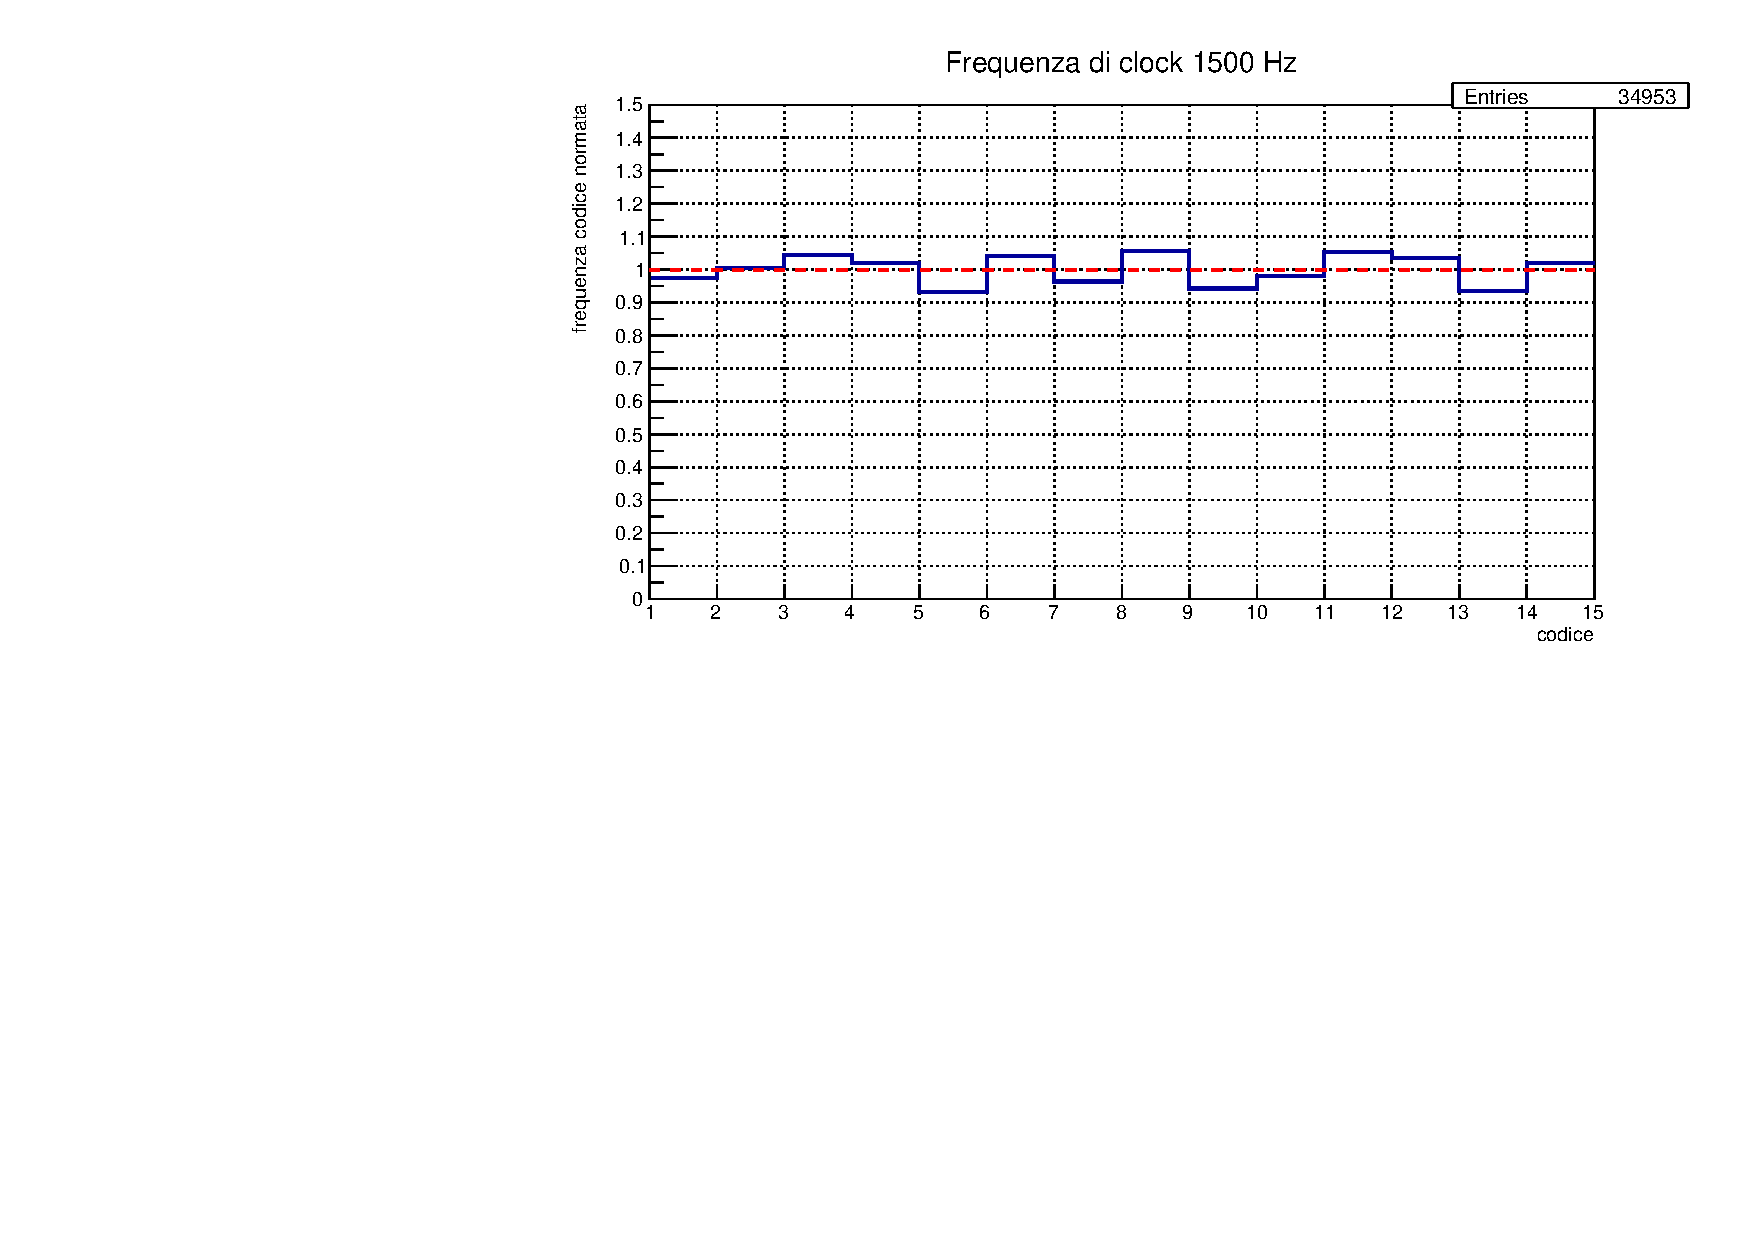
\includegraphics[width=0.48\textwidth]{analysis/output/dnl_5_1500hz_bars.pdf}
\label{fig:graph_dnl_1500_hz}
%6
\caption{$\sigma = 0.063$}
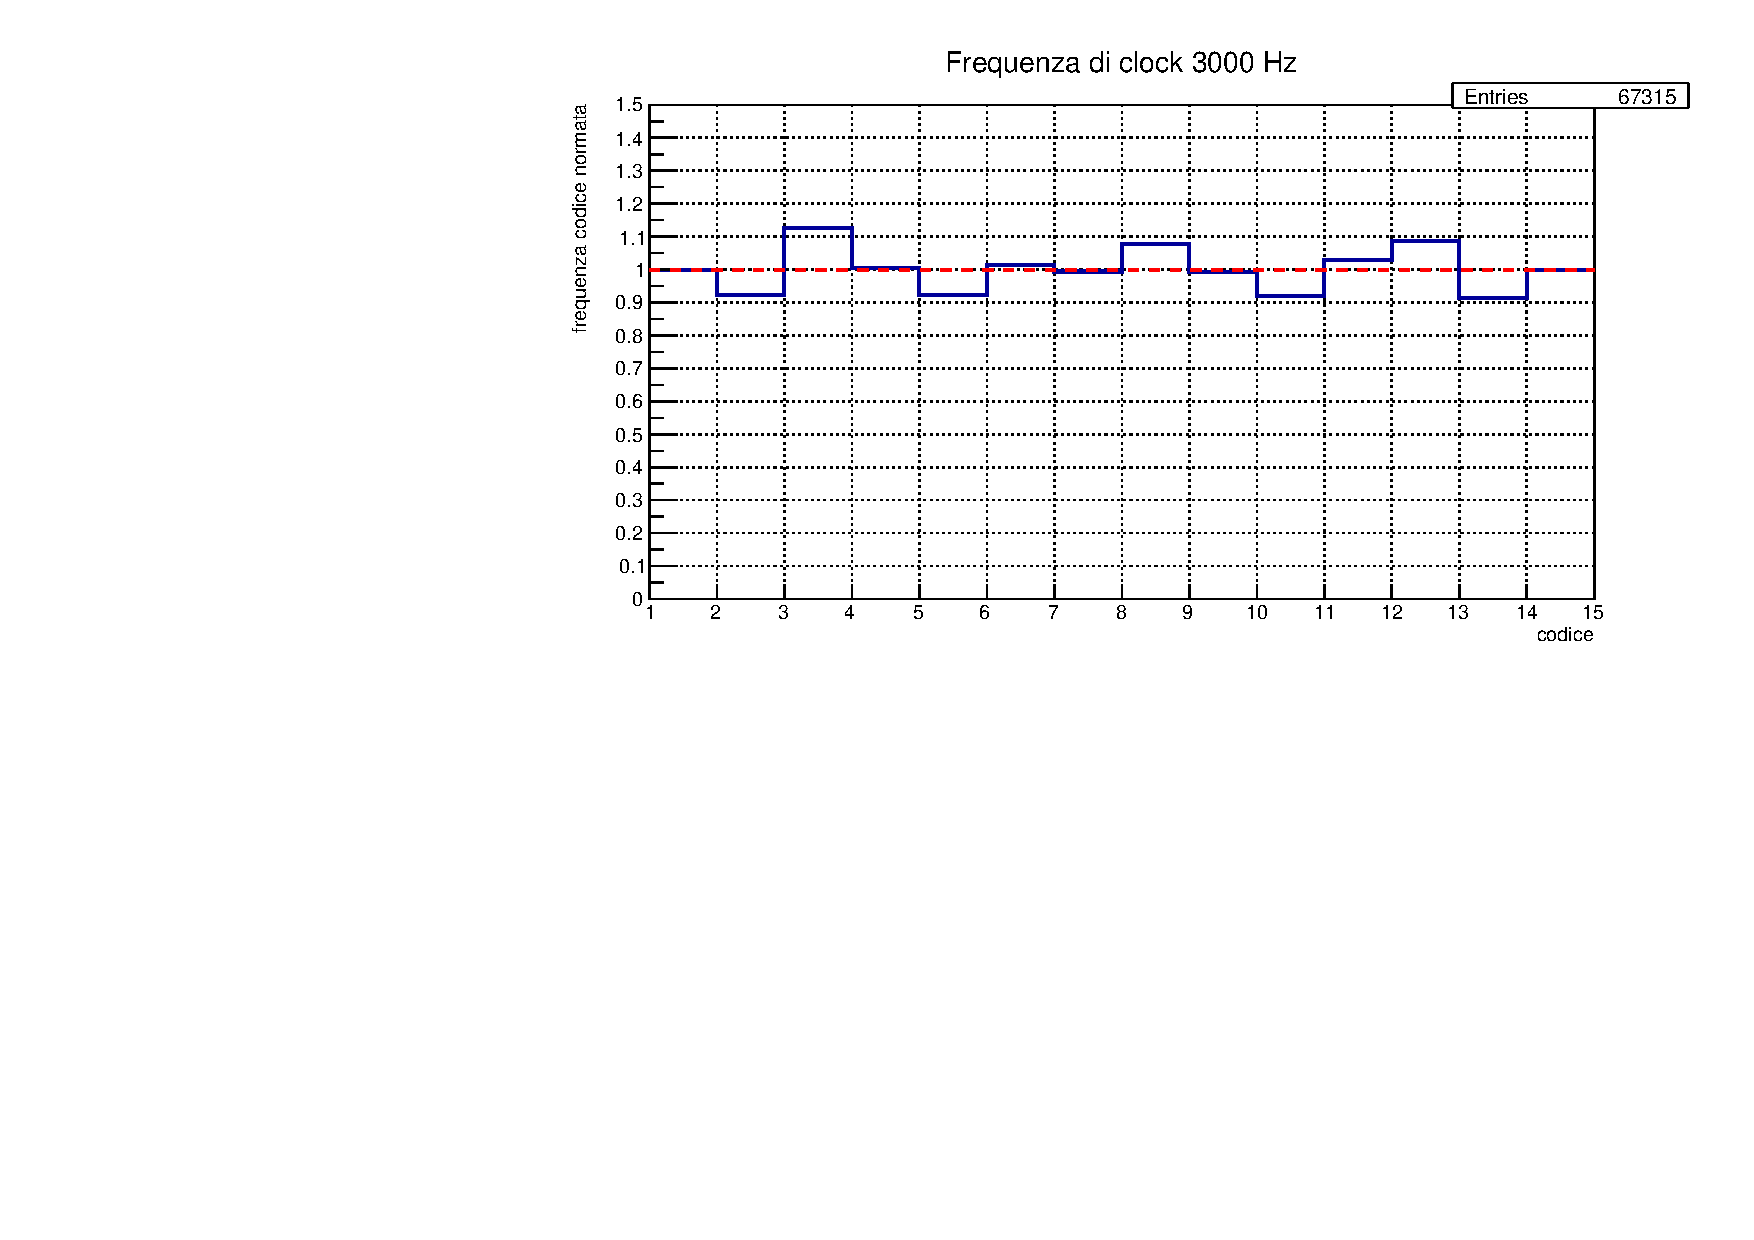
\includegraphics[width=0.48\textwidth]{analysis/output/dnl_6_3000hz_bars.pdf}
\label{fig:graph_dnl_3000_hz}
%7
\caption{$\sigma = 0.099$}
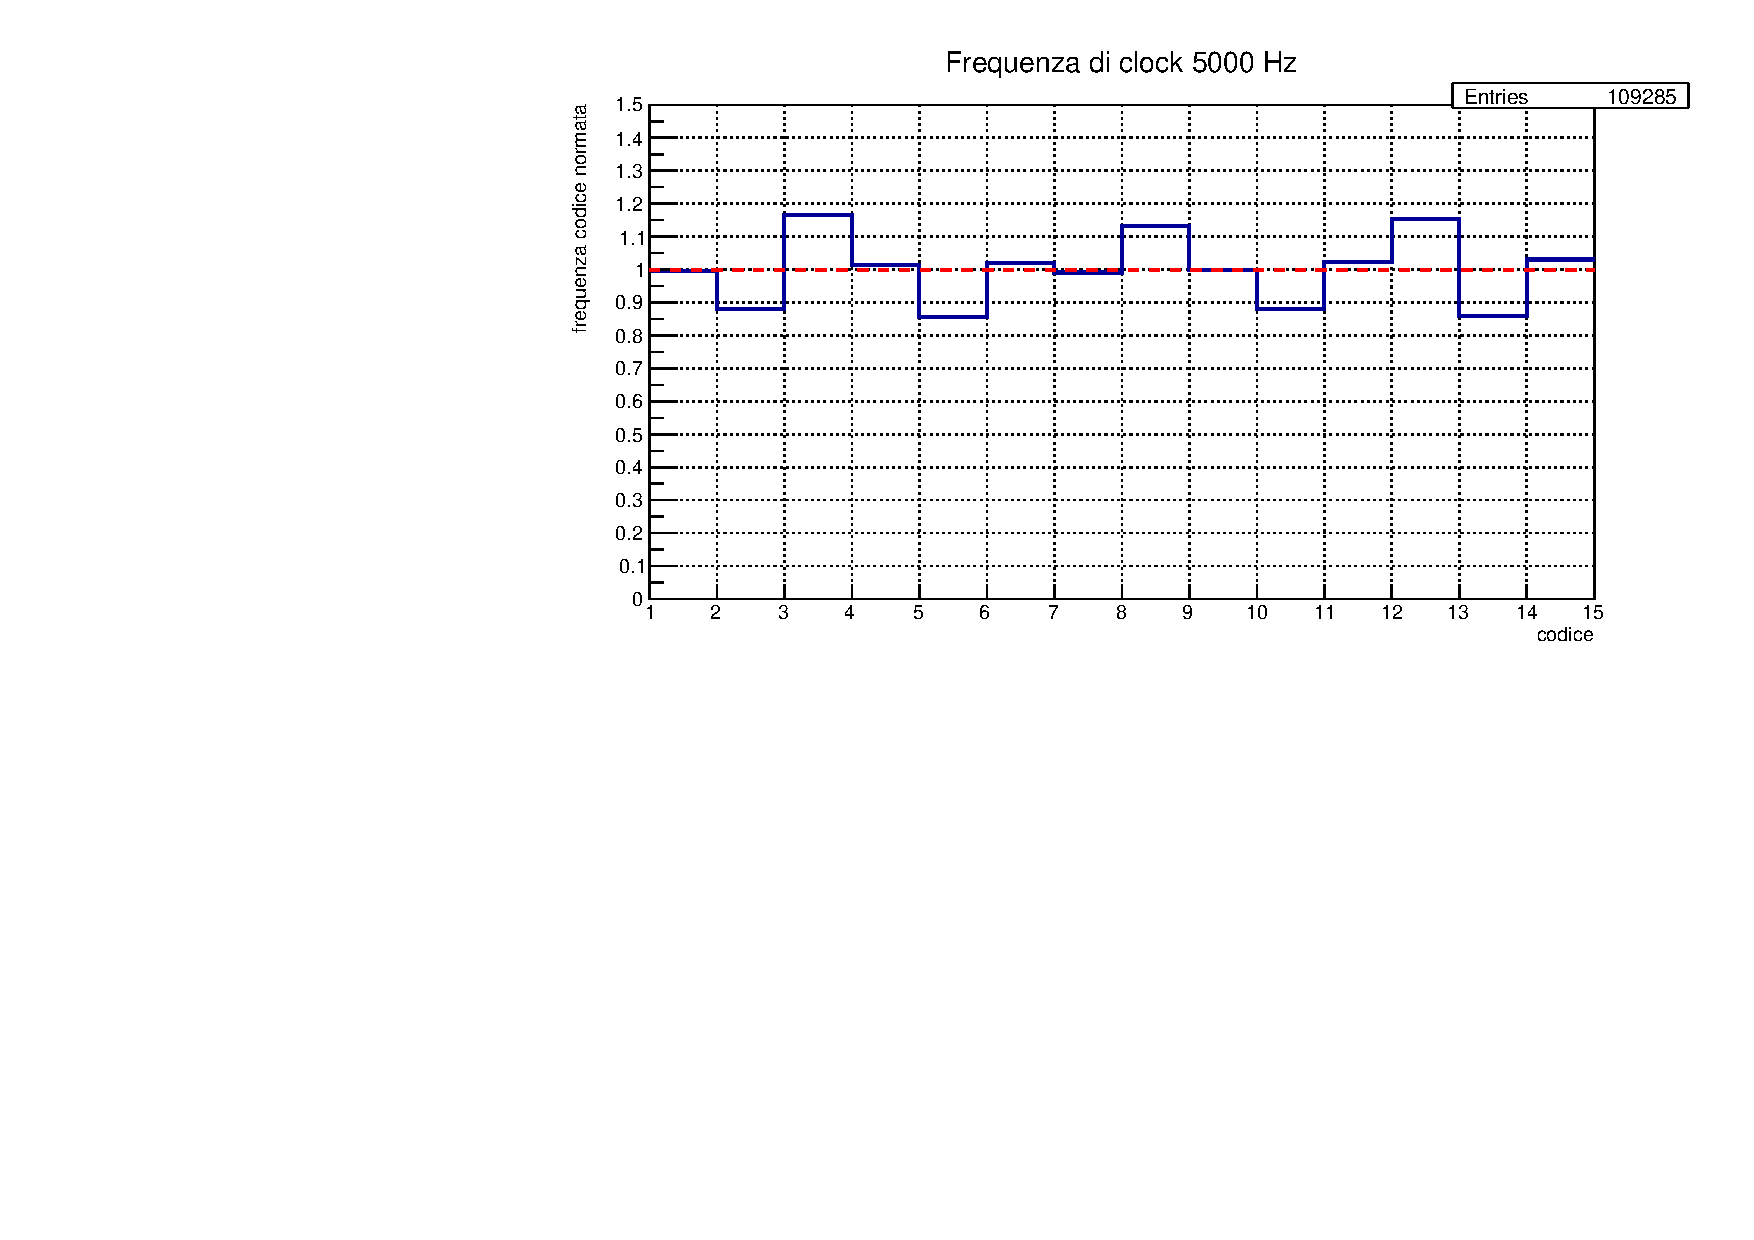
\includegraphics[width=0.48\textwidth]{analysis/output/dnl_7_5000hz_bars.pdf}
\label{fig:graph_dnl_5000_hz}
%8
\caption{$\sigma = 0.16$}
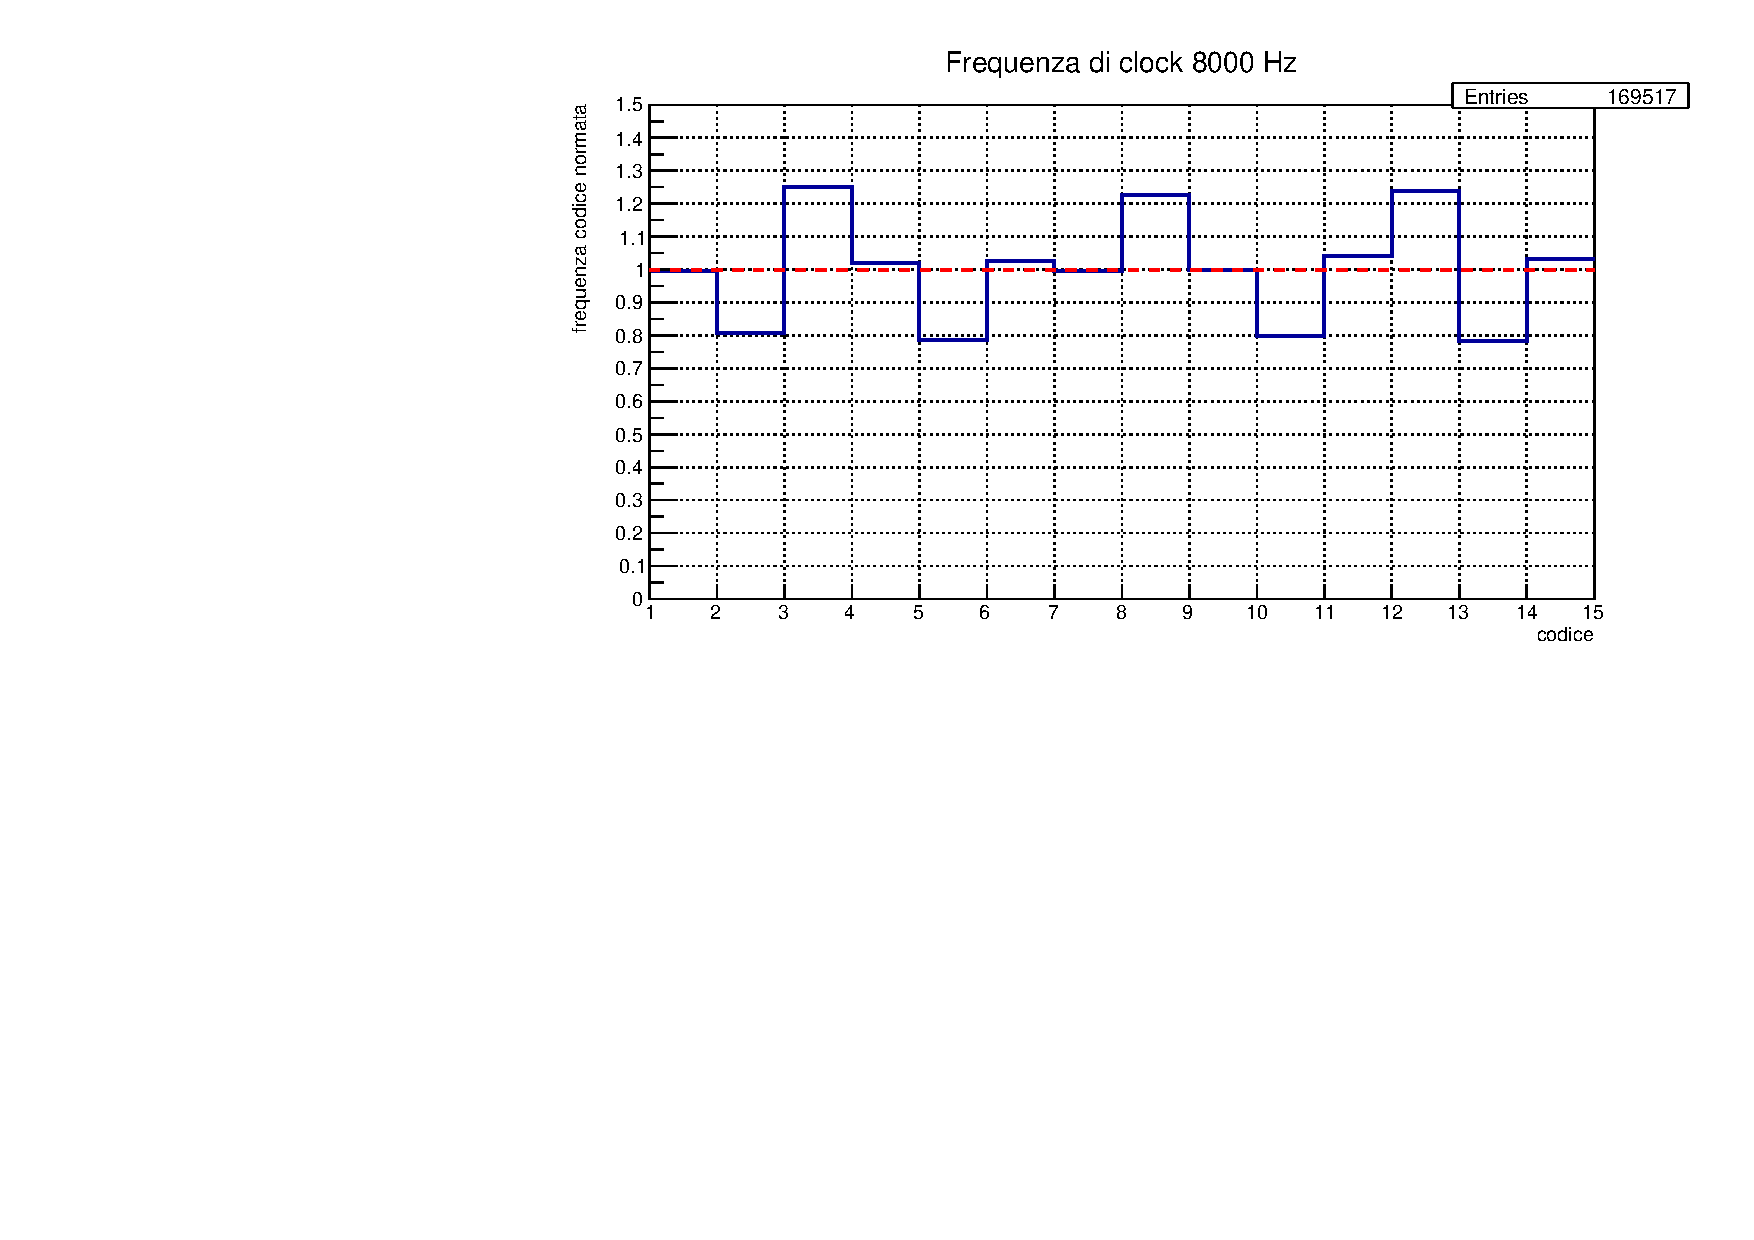
\includegraphics[width=0.48\textwidth]{analysis/output/dnl_8_8000hz_bars.pdf}
\label{fig:graph_dnl_8000_hz}

\end{center}
\end{figure}

\subsubsection{Distribuzione della deviazione standard}

\begin{figure}[H]%[!ht]
\begin{center}
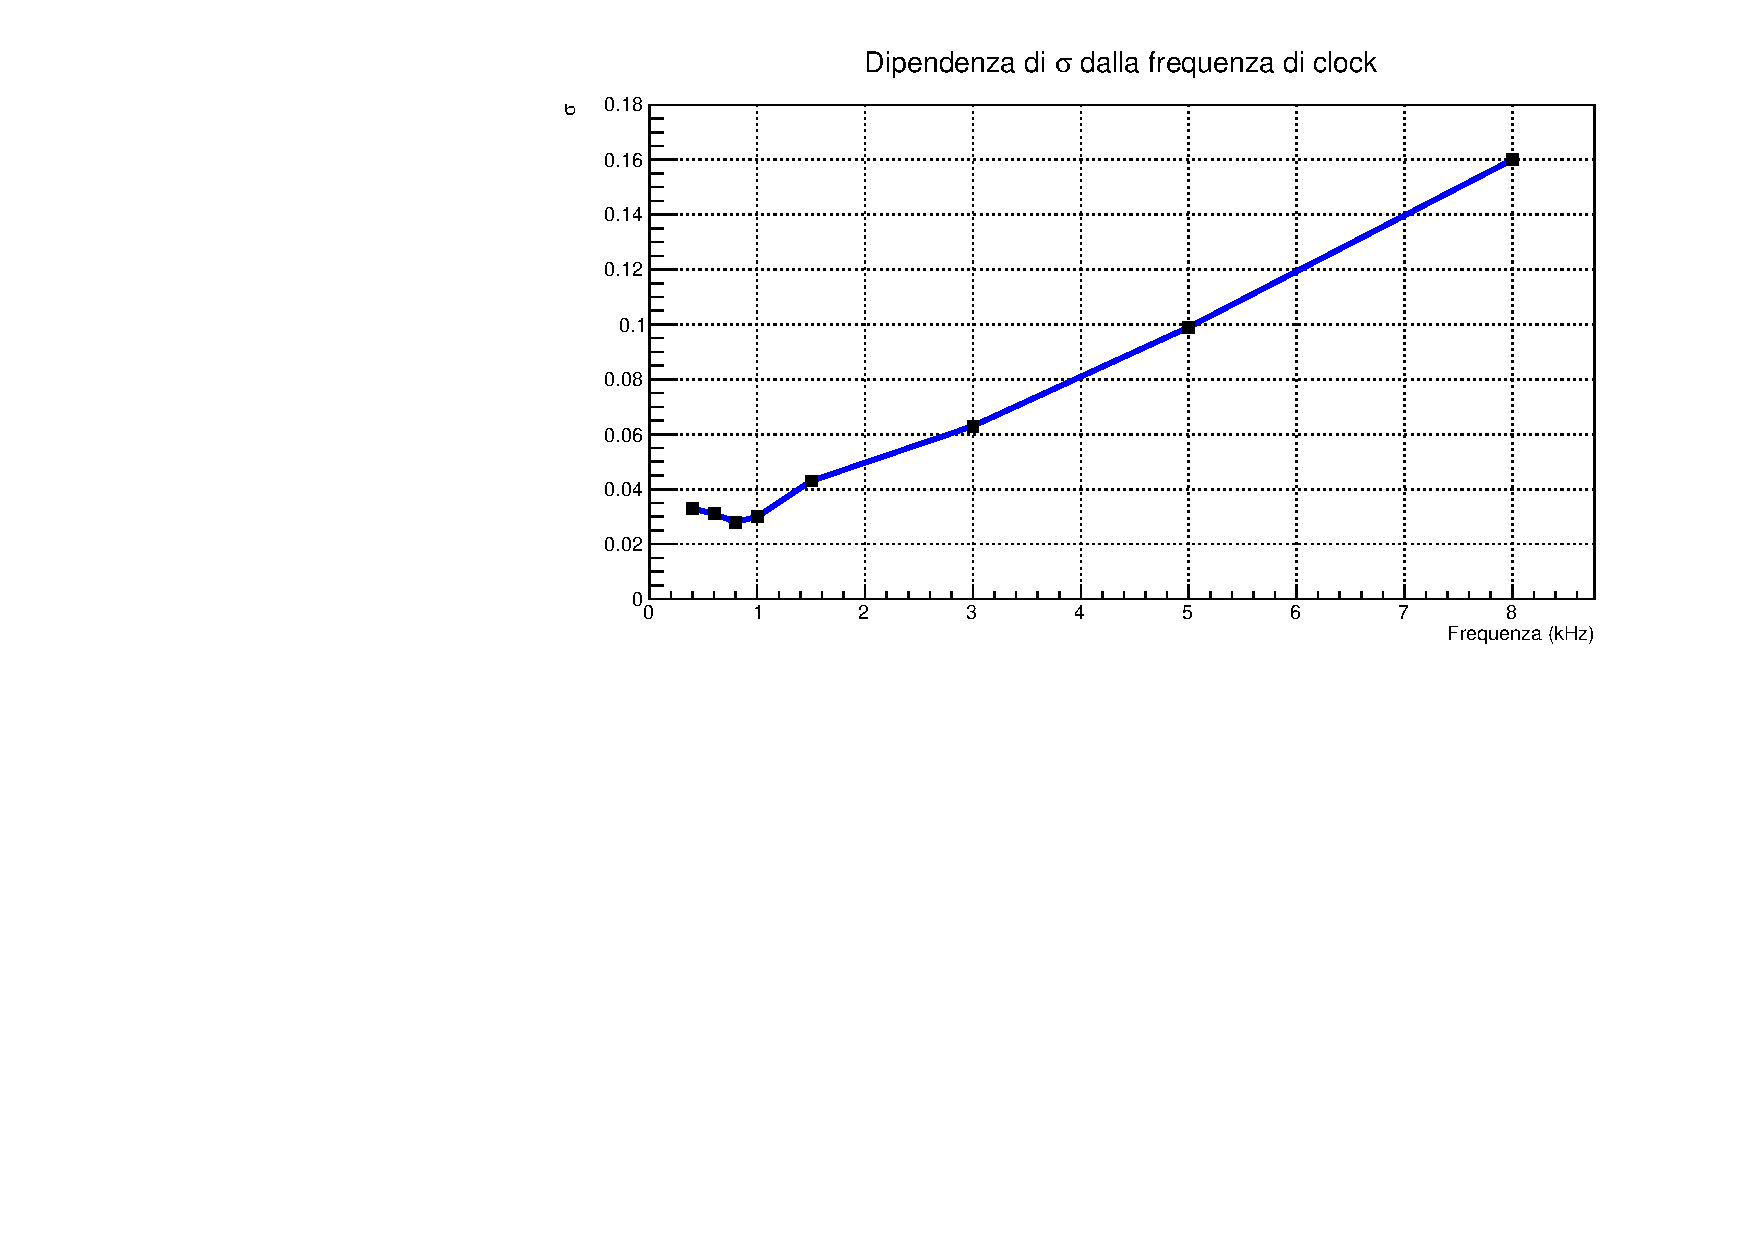
\includegraphics[width=0.50\textwidth]{analysis/output/dnl_sigma_pdf}
\caption{Letture mancanti}
\label{fig:graph_dnl_sigma}
\end{center}
\end{figure}


%%%%%%%%%%%%%%%%%%%%%%%%%%%%%%%%%%%%%%%%%%%%%%%%%%%%%%%%%%%

\subsection{Valori mancanti}

\begin{figure}[H]%[!ht]
\begin{center}
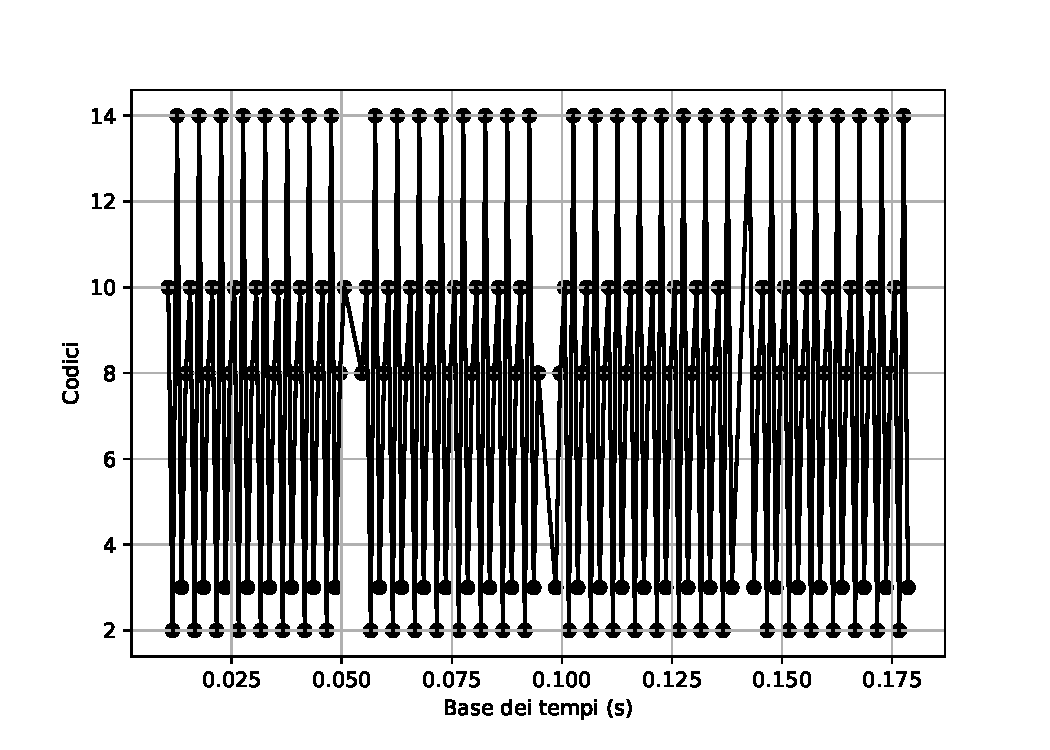
\includegraphics[width=0.50\textwidth]{analysis/output/letture_mancanti.pdf}
\caption{Letture mancanti}
\label{fig:missing}
\end{center}
\end{figure}

%%%%%%%%%%%%%%%%%%%%%%%%%%%%%%%%%%%%%%%%%%%%%%%%%%%%%%%%%%%%%
\section{Discussione dei risultati e conclusioni}
Testo


\begin{figure*}[t]%[t]
\centering
\begin{center}
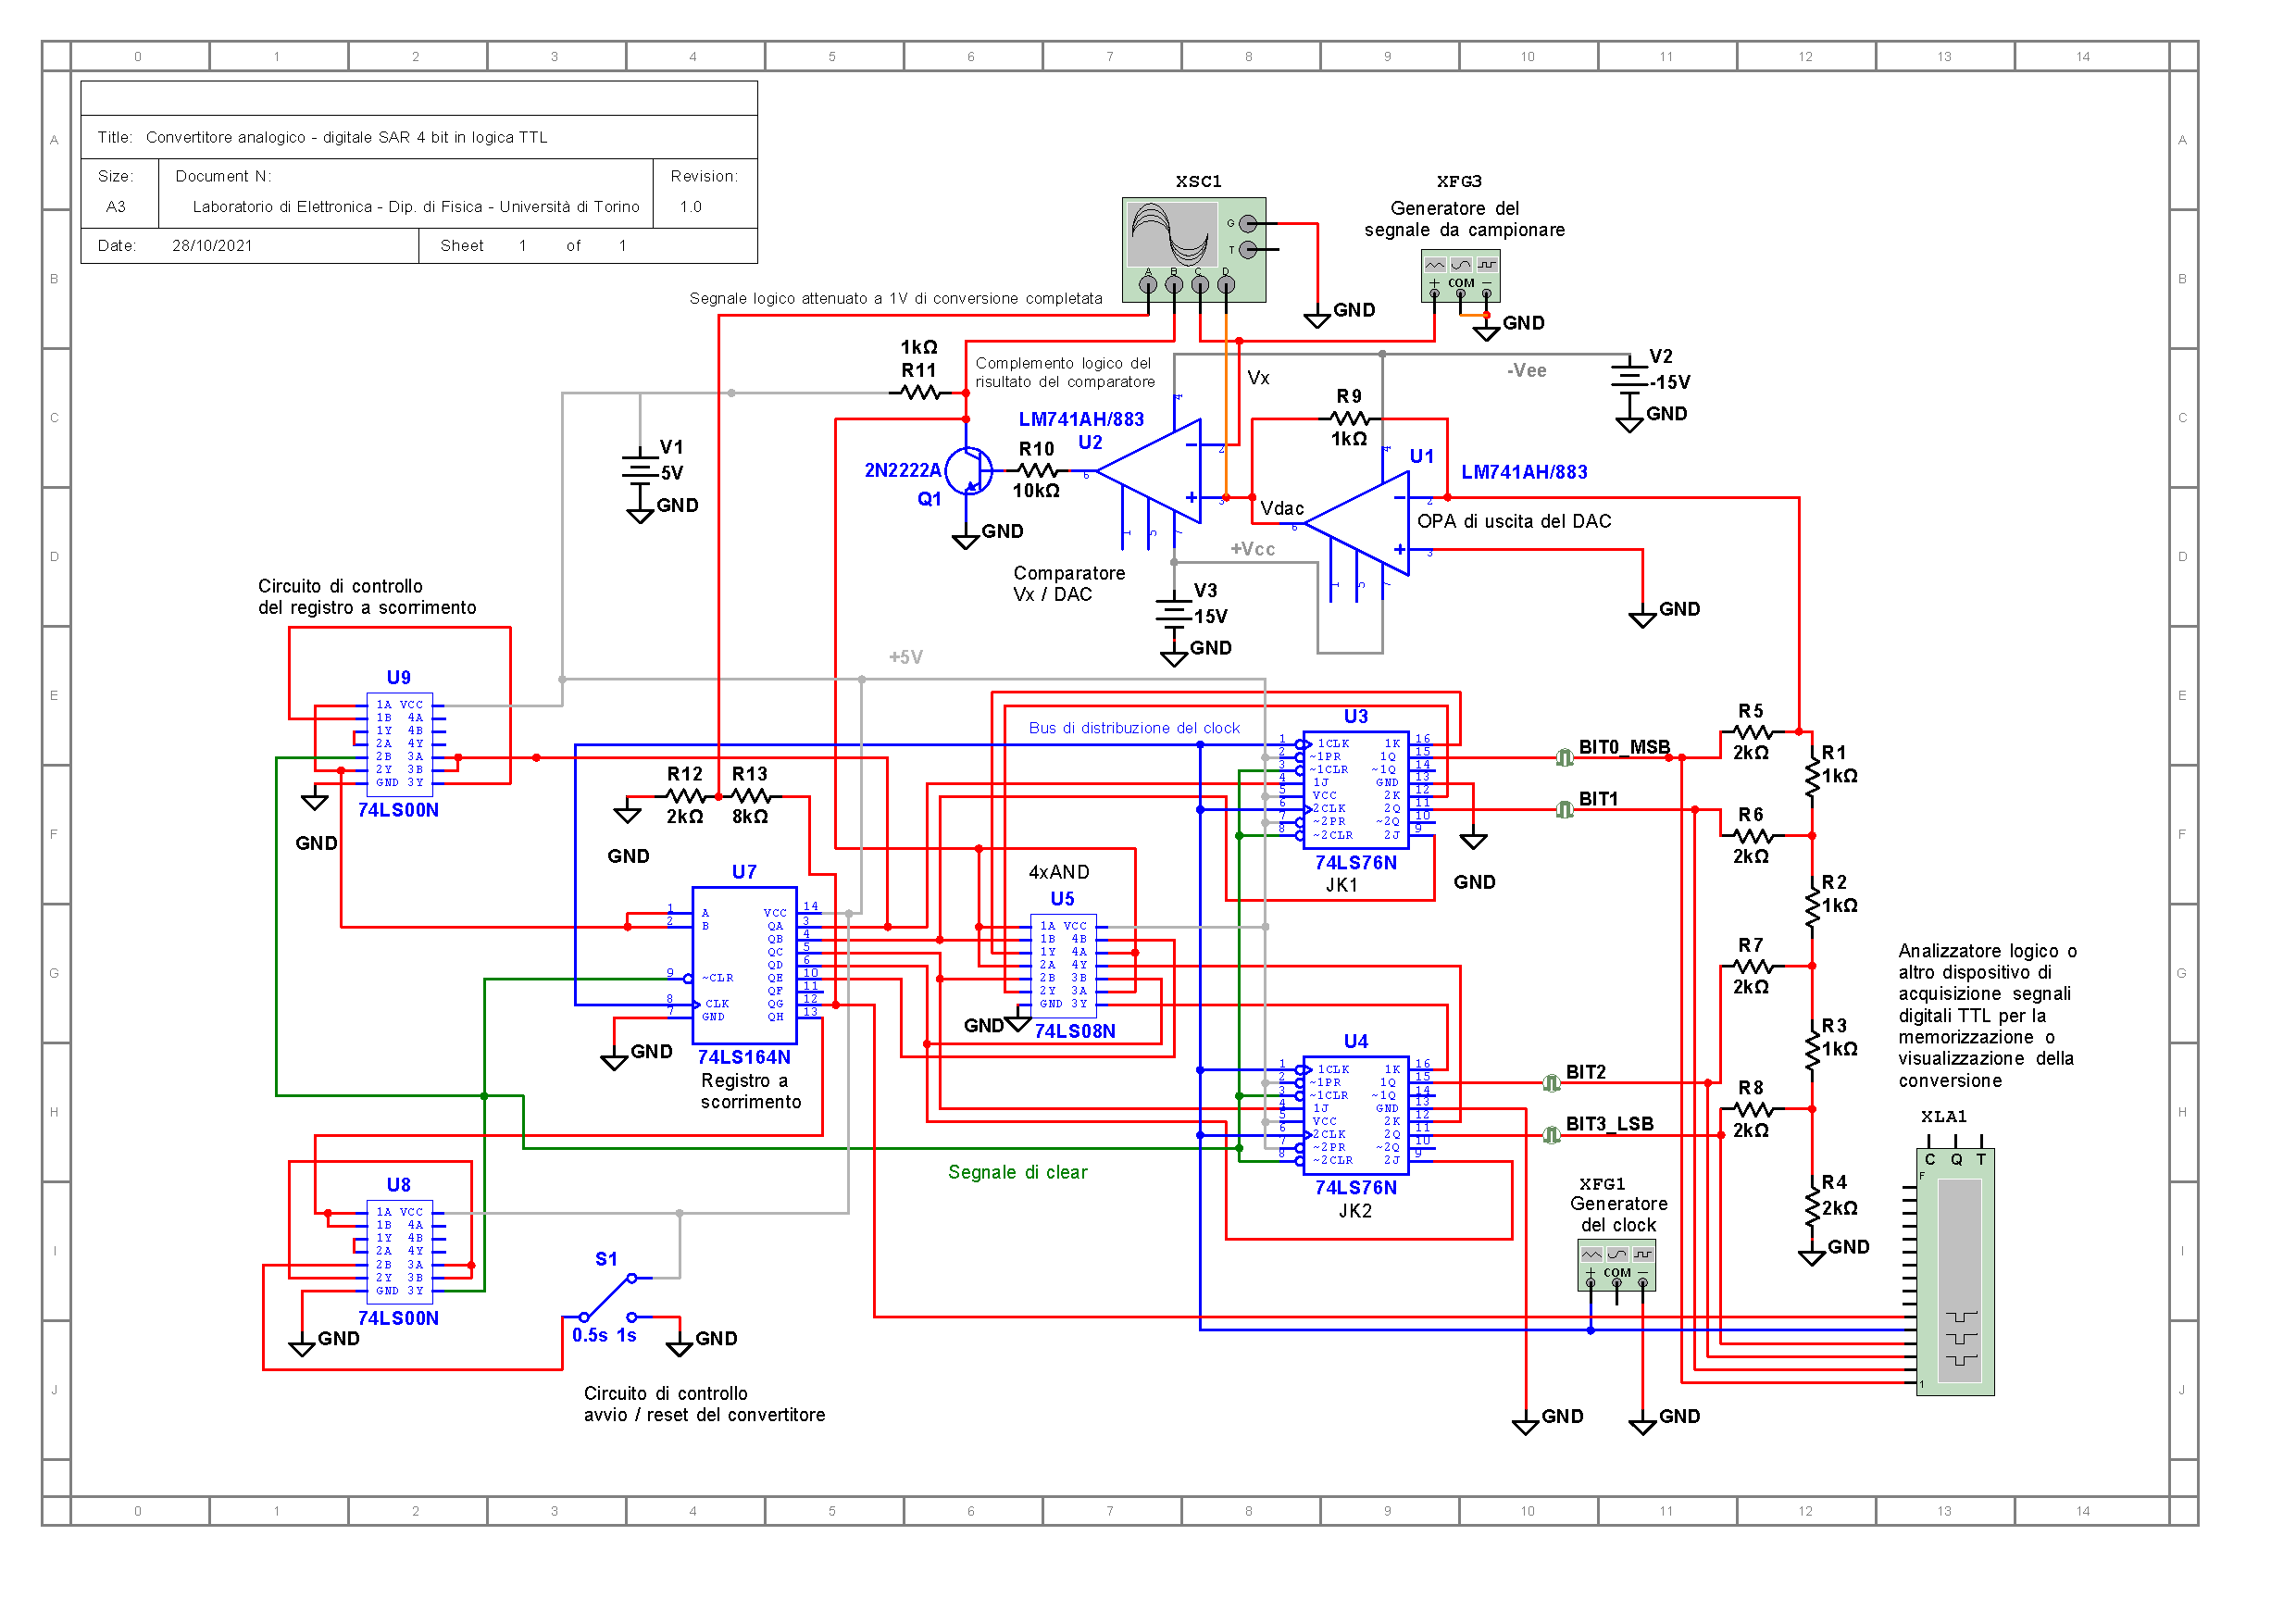
\includegraphics[trim = {0 0 50 0}, width=1.40\textwidth, angle=90]{sch-simulations/digital/output/Schema_convertitore_completo.pdf}
\end{center}
\caption{Schema elettrico completo del convertitore ADC SAR 4 bit}
\label{fig:circuit_sarCompleteSchematic}
\end{figure*}



%%%%%%%%%%%%%%%%%%%%%%%%%%%%%%%%%%%%%%%%%%%%%%%%%%%%%%%%%%%%%
%% Appendice
%%%%%%%%%%%%%%%%%%%%%%%%%%%%%%%%%%%%%%%%%%%%%%%%%%%%%%%%%%%%%

\clearpage

\begin{appendices}

\section{Tabella calibrazione DAC}

\centering
\begin{tabular}{cc}
binario & V $ \pm 0.1 \ V $ \\ \hline
0       & 0.0                          \\
1       & -0.3                       \\
10      & -0.6                       \\
11      & -0.9                       \\
100     & -1.2                       \\
101     & -1.6                       \\
110     & -1.9                       \\
111     & -2.2                       \\
1000    & -2.5                       \\
1001    & -2.8                       \\
1010    & -3.1                       \\
1011    & -3.4                       \\
1100    & -3.7                       \\
1101    & -4.0                       \\
1110    & -4.3                       \\
1111    & -4.6
\vspace{5 mm}
%\caption{}
\label{tab:calibrazione_dac}
\end{tabular}


\section{Tabella calibrazione ADC}

\begin{tabular}{cc}
binario & $V_{min}  \pm 0.1 \ V$ \\ \hline
1111    & -3.2                  \\
1110    & -3.0                  \\
1101    & -2.7                  \\
1100    & -2.5                  \\
1011    & -2.3                  \\
1010    & -2.1                  \\
1001    & -1.9                  \\
1000    & -1.7                  \\
111     & -1.5                  \\
110     & -1.3                  \\
101     & -1.0                  \\
100     & -0.8                  \\
11      & -0.7                  \\
10      & -0.5                  \\
1       & -0.2                  \\
0       & 0.0
\vspace{5 mm}
%\caption{}
\label{tab:calibrazione_adc}
\end{tabular}


\end{appendices}

%%%%%%%%%%%%%%%%%%%%%%%%%%%%%%%%%%%%%%%%%%%%%%%%%%%%%%%%%%%%%
%% Indice e Bibliografia 
%%%%%%%%%%%%%%%%%%%%%%%%%%%%%%%%%%%%%%%%%%%%%%%%%%%%%%%%%%%%%

\clearpage
\newpage

\tableofcontents % Indice

\newpage

\printbibliography % Bibliografia

\end{document}